%% LyX 2.3.6.2 created this file.  For more info, see http://www.lyx.org/.
%% Do not edit unless you really know what you are doing.
\documentclass[english,AER, finalmode]{AEA}
\usepackage[latin9]{inputenc}
\setcounter{secnumdepth}{3}
\setcounter{tocdepth}{3}
\synctex=-1
\usepackage{color}
\usepackage{units}
\usepackage{mathrsfs}
\usepackage{url}
\usepackage{amsmath}
\usepackage{amssymb}
\usepackage{graphicx}
\usepackage{setspace}
\usepackage[authoryear]{natbib}

\makeatletter

%%%%%%%%%%%%%%%%%%%%%%%%%%%%%% LyX specific LaTeX commands.
\newcommand{\noun}[1]{\textsc{#1}}
%% Because html converters don't know tabularnewline
\providecommand{\tabularnewline}{\\}

%%%%%%%%%%%%%%%%%%%%%%%%%%%%%% Textclass specific LaTeX commands.
\newtheorem{lemma}{Lemma}
\newtheorem{theorem}{Theorem}
\newtheorem{conjecture}{Conjecture}
\newenvironment{lyxlist}[1]
	{\begin{list}{}
		{\settowidth{\labelwidth}{#1}
		 \setlength{\leftmargin}{\labelwidth}
		 \addtolength{\leftmargin}{\labelsep}
		 \renewcommand{\makelabel}[1]{##1\hfil}}}
	{\end{list}}
\newtheorem{proposition}{Proposition}

%%%%%%%%%%%%%%%%%%%%%%%%%%%%%% User specified LaTeX commands.

%\usepackage[english]{babel}
%\usepackage{amsmath,amssymb,amsfonts,amsthm}
%\usepackage[scaled=.90]{helvet}
%\usepackage{mathpazo}
\usepackage[margin=1in]{geometry}

\usepackage[hidelinks]{hyperref}
\usepackage{natbib}
\usepackage{array}
%\usepackage{mathpple}
%\usepackage{stmaryrd}
%\usepackage[T1]{fontenc}
%\usepackage{palatino}
%\usepackage[svgnames]{xcolor}
%\usepackage{mathtools}

\usepackage[bottom]{footmisc}
\interfootnotelinepenalty=2147483647

\usepackage{graphicx}
\usepackage[export]{adjustbox}
\DeclareGraphicsExtensions{.pdf,.jpeg,.png,.eps}
\usepackage{enumitem}
\usepackage{changepage}
\strictpagecheck

\makeatletter
\newcounter{parentnumber} 

\usepackage{booktabs}
\newcommand{\specialcell}[2][c]{%
  \begin{tabular}[#1]{@{}c@{}}#2\end{tabular}}
\usepackage{multirow}


\author{Ahmad  Lashkaripour and Volodymyr Lugovskyy\thanks{Lashkaripour: Indiana University (email: ahmadlp@gmail.com); Lugovskyy: Indiana University (email:vlugovsk@indiana.edu). We are grateful to James Anderson, Adina Ardelean, Dominick Bartelme, Kerem Cosar, Arnaud Costinot, Farid Farrokhi, Harald Fadinger, Fabio Ghironi, David Hummels, Kala Krishna, Konstantin Kucheryavyy, Danial Lashkari, Nuno Limao, Gary Lyn, Ralph Ossa, James Rauch, Andr�s Rodr�guez-Clare, Kadee Russ, Peter Schott, Alexandre Skiba, Anson Soderbery, Robert Staiger, Jonathan Vogel and conference participants at the Midwest Trade Meetings, Chicago Fed, UECE Lisbon Meetings, 2017 NBER ITI Summer Institute, 2019 WCTW, Indiana University, Purdue University, SIU, IBA, Boston College, University of Mannheim, and University of Michigan for helpful comments and suggestions. We thank Nicolas de Roux and Santiago Tabares for providing us with data on the Colombian HS10 product code changes over time. We are grateful to Fabio Gomez for research assistance. Lugovskyy thanks Indiana University SSRC for financial support. All errors are our own. }}


\date{June 2023}
%\date{December 2019}
%\setlength\parskip{10pt}

\makeatother

\usepackage{bbm}

\usepackage{xr}
\externaldocument{Online_Appendix}

\makeatother

\usepackage{babel}
\providecommand{\conjecturename}{Conjecture}
\providecommand{\lemmaname}{Lemma}
\providecommand{\propositionname}{Proposition}
\providecommand{\theoremname}{Theorem}

\begin{document}
\title{Profits, Scale Economies, and \\ the Gains from Trade and Industrial
Policy}
\begin{abstract}
This paper examines the efficacy of second-best trade restrictions
at correcting misallocation in the domestic economy. To this end,
we derive sufficient statistics formulas for first-best and second-best
optimal policies in an important class of quantitative trade models
where misallocation stems from scale economies or profit-generating
markups. We then estimate the essential parameters of the model and
apply our optimal policy formulas to quantify the ex-ante gains from
trade and industrial policy among major countries. Our estimates reveal
$(i)$ that standalone trade policy measures are remarkably ineffective
at correcting misallocation; $(ii)$unilateral adoption of corrective
industrial policies is also ineffective as it leads to immiserizing
growth; but $(iii)$ industrial policies coordinated internationally
via deep agreements are more transformative than any unilateral policy
alternative.
\end{abstract}
\maketitle
The United States will likely adopt an explicit industrial policy
in the coming decade. Similar developments are well underway in other
countries (\citet{aiginger2020rebirth}). And with industrial policy
back on the scene, we are witnessing a revival of old-but-questionable
trade policy practices. Govenments are often turning to protectionist
trade policy measures to pursue their industrial policy objectives---as
manifested by the United States \emph{National Trade Council}'s mission
or the Chinese, \emph{Made in China 2025} initiative.\footnote{See \citet{bhagwati1988protectionism} and \citet{irwin2017clashing}
for a historical account of trade restrictions being used by governments
to promote their preferred industries. A prominent example dates back
to 1791, when Alexander Hamilton approached Congress with \emph{``the
Report on the Subject of Manufactures},'' encouraging the implementation
of protective tariffs and industrial subsidies. These policies were
intended to help the US economy catch up with Britain.}

These developments have sparked new interest in old-but-open questions
regarding trade and industrial policy. For instance: $\boldsymbol{(i)}$
Is trade policy an effective tool for correcting misallocation in
the domestic economy? $\boldsymbol{(ii)}$ If not, should governments
undertake \emph{unilateral} domestic policy interventions to correct
misallocation? or $\boldsymbol{(iii)}$ should they coordinate their
industrial policies via a deep trade agreement?

To answer these questions, we characterize optimal trade and industrial
policies in an important class of multi-industry, multi-country quantitative
trade models where misallocation occurs due to scale economies or
profit-generating markups. Guided by theory, we estimate the key parameters
that govern the welfare consequences of trade and industrial policy
in open economies. We then combine our estimated parameters with optimal
policy formulas to quantify the ex-ante gains from trade and industrial
policy among 43 major countries.

Our estimation reveals that trade policy is remarkably ineffective
at correcting misallocation, reflecting a deep tension between allocative
efficiency and terms of trade. Unilateral adoption of corrective industrial
policies can also backfire as it often triggers \emph{immiserizing
growth}. These considerations, we argue, may have spurred a global
\emph{race to the bottom}, wherein governments either avoid corrective
industrial policies or pair them with hidden trade barriers. A deep
agreement can remedy this problem and deliver welfare gains that are
more transformative than any unilateral policy intervention.

Section \ref{sec:Theoretical-Framework} presents our theoretical
framework. Our baseline model is a generalized multi-industry \citet{Krugman1980}
model that features a non-parametric utility aggregator across industries
and a nested CES utility aggregator within industries. This specification
has an appealing property wherein the degrees of firm-level and country-level
market love-for-variety can diverge. We analyze both the restricted
and free entry cases of the model to distinguish between the \emph{short-run}
and \emph{long-run} consequences of policy. With a reinterpretation
of parameters, our baseline framework also nests $(a)$ the multi-industry
\citet{Melitz2003}-Pareto model, and $(b)$ the multi-industry \citet{Eaton2002}
model with industry-level Marshallian externalities. We later extend
our baseline model to accommodate non-parametric input-output linkages.

Section \ref{sec:The-Structure-of-Optimal-Policy} derives sufficient
statistics formulas for \emph{first-best} and \emph{second-best} trade
and industrial policies. Unilaterally optimal policies in our framework
pursue two objectives: First, they seek to improve the home country's\emph{
terms-of-trade (ToT)} vis-\`a-vis the rest of the world. Second,
they seek to restore \emph{allocative efficiency} in the domestic
economy by reallocating workers towards high-returns to scale or high-profit
industries.

The \emph{first-best} optimal policy consists of misallocation-blind
import tariffs and export subsidies that purely maximize ToT gains.
Allocative efficiency under the first-best is restored via domestic
Pigouvian subsidies.\footnote{The optimal subsidy rate in each industry equals the inverse of the
industry-level scale elasticity or markup.} While these insights resonate with the targeting principle, our optimal
policy formulas have other implications worth highlighting. First,
even though 1st-best trade policies are blind to misallocation (the
dispersion in scale elasticities), they depend on the overall strength
of scale economies (the level of scale elasticities). Second, the
optimal tariff formula is input-output-blind provided that export
subsidies are assigned optimally.\footnote{Specifically, optimal import tariffs are equal to the inverse export
supply elasticity regardless of input-output relationships. Consequently,
in the absence of profits and scale economies, optimal tariffs become
uniform when export subsidies are set optimally---revealing that
the uniformity result in \citet{costinot2015comparative} extends
to environments with input-output linkages.} 

Our \emph{second-best} trade policy formulas apply to scenarios where
governments are reluctant to use industrial subsidies for correcting
misallocation---the root of which could be political pressures or
institutional barriers.\footnote{Trade policy has been regularly used---in place of domestic industrial
policy---to promote critical industries (\citet{bhagwati1988protectionism};
\citet{harrison2010trade}; \citet{irwin2017clashing}). Relatedly,
see \citet{lane2020new} for a historical account of various industrial
policy practices around the world.} Second-best trade tax-cum-subsidies are composed of two elements:
a neoclassical ToT-improving component and a misallocation-correcting
component. The former aims to restrict relative exports in nationally
differentiated industries. The latter seeks to restrict imports and
promote exports in high-returns-to-scale industries, mimicking the
first-best Pigouvian subsidies.

Section \ref{sec: Tension}, guided by our optimal policy framework,
puts forth two conjectures concerning the efficacy of trade and industrial
policy: First, if industry-level trade and scale elasticities exhibit
a strong negative correlation, standalone trade policy measures deliver
limited welfare gains even when set optimally---reflecting their
inability to strike a balance between ToT-improving and misallocation-correcting
objectives.\footnote{In some canonical cases, optimal second-best trade policies are even
industry-blind---unable to beneficially correct inter-industry misallocation
or manipulate the ToT on an industry-by-industry basis.} Second, in these conditions, unilateral scale (or markup) correction
via industrial policy can cause \emph{immiserizing growth }due to
adverse ToT effects. Consequently, shallow trade agreements may be
insufficient for reaching global efficiency. Once governments agree
to abandon inefficient trade restrictions under a shallow agreement,
they become tangled in a coordination game involving corrective industrial
policies. The outcome of this game is a \emph{race to the bottom}
wherein governments are reluctant to implement corrective industrial
policies without violating their commitments to free trade. A deep
agreement can remedy this problem.

To test these conjectures, Section \ref{sec:Estimation} estimates
the structural parameters necessary for ex-ante policy evaluation.
Our optimal policy formulas reveal that the sufficient statistics
for measuring policy outcomes include observables and two sets of
parameters: $(i)$ industry-level scale elasticities that govern the
extent of misallocation and $(ii)$ industry-level trade elasticities
that control the scope for ToT manipulation. In our generalized \citet{Krugman1980}
model, scale elasticities reflect the degree of \emph{love-for-variety}
whose social benefits are not internalized by firms' entry decisions;
and trade elasticities represent the degree of national product differentiation.
We recover both elasticities from firm-level demand parameters, which
are estimated by fitting a structural demand function to the universe
of Colombian import transactions covering over 225,000 firms from
251 countries. Our identification strategy leverages high-frequency
data on import transactions and exchange rates to construct a shift-share
instrument that measures exposure to aggregate exchange rate fluctuations
at the firm-product-year level.\footnote{We develop this identification strategy to overcome challenges that
are difficult to resolve with standard demand estimation techniques.
Firm-level demand estimation techniques from the Industrial Organization
literature leverage information on observed product characteristics,
which are unavailable at the scale we conduct our estimation. Also,
unlike traditional \emph{country-level} import demand estimations,
we cannot rely on tariff data for identification, as tariff rates
do not vary sufficiently among firms from the same country.} This estimation strategy is well-suited for our end goal of policy
evaluation as it separately identifies the scale elasticities from
trade elasticities, accurately pinpointing their covariance.

Section \ref{sec:Quantifying-the-Gains} combines our estimated scale
and trade elasticity parameters, our optimal policy formulas, and
macro-level data from the 2014 World Input-Output Database to quantify
the (maximal) ex-ante gains from policy among 43 major economies.
Our analysis delivers three main findings.

First, we find that trade policy is remarkably ineffective at correcting
misallocation in the domestic economy---even without factoring in
the cost of retaliation by trading partners. Under free entry, second-best
export subsidies and import taxes can raise the average country's
real GDP by only 1.19\%, which amounts to less than $\nicefrac{4}{10}$
of the gains attainable under the unilaterally first-best policy.
Third-best import taxes are even less effective as a standalone policy,
raising real GDP by a mere 0.63\%. These findings corroborate the
argument that trade policy has difficulty striking a balance between
ToT and misallocation-correcting objectives. 

Second, the unilateral adoption of corrective industrial policies
triggers severe immiserizing growth in most countries. The average
country's real GDP declines by 2.7\% if they implement scale-correcting
subsidies without reciprocity by trading partners. Aversion to these
consequences, we argue, may have spurred a global race to the bottom
in industrial policy implementation. To escape immiserizing growth,
governments either avoid corrective policies or pair them with hidden
trade barriers that breach shallow trade cooperation.\footnote{The Chinese government, for instance, pairs its domestic subsidies
with hidden export taxes. These hidden barriers are applied via partial
value-added tax rebates and are designed to restore China's ToT (\citet{garred2018persistence}). }

Third, deep agreements can remedy the race to the bottom and deliver
welfare gains that are more transformative than any unilateral intervention.
To offer some perspective, corrective industrial policies coordinated
via a deep agreement can elevate the average country's real GDP by
3.2\%. These welfare gains rival the already-realized gains from shallow
agreements for most countries. They, moreover, exceed any welfare
gains achievable through unilateral trade or industrial policy interventions---even
not considering that unilateralism often backfires in the form of
retaliation by trading partners.\medskip{}

\emph{Related Literature}---Our theory relates to an emerging literature
on optimal policy in \emph{distorted} open economies. In a concurrent
paper, \citet{BCDR2017} characterize the first-best optimal policy
for a small open economy in a multi-sector Ricardian model with Marshallian
externalities. Relatedly, \citet{haaland2016optimal} characterize
optimal policy for a small open economy in two-by-two Krugman and
Melitz models.\footnote{\citet{demidova2009trade} and \citet{felbermayr2013optimal} characterize
optimal tariffs in a \emph{single industry} Melitz-Pareto model. The
single industry assumption ensures that markets are efficient (\citet{dhingra2019monopolistic})
and import and export taxes are equivalent (the Lerner symmetry).
So, the unilaterally first-best can be reached with import tariffs
alone. \citet{costinot2016micro} examine optimal policy in the\emph{
single industry} Melitz-Pareto model from a different lens, characterizing
optimal \emph{firm-level} taxes.} Beyond optimal policy, \citet{campolmi2018trade} employ a two-sector
Melitz-Pareto model to elucidate the trade-offs facing countries that
join shallow and deep trade agreements.\footnote{Other papers have also used new or quantitative trade models to analyze
piecemeal policy reforms in distorted economies or optimal policy
in \emph{non-distorted} economies---e.g., \citet{costinot2014trade,campolmi2014trade,costinot2015comparative,bagwell2015trade,caliendo2015tariff,demidova2017trade,beshkar2017interdependence,beshkar2020cost}.} Our analysis of \emph{second-best} trade policies speaks to an older
literature emphasizing the firm-delocation rationale for trade restrictions
(e.g., \citet{venables1987trade,ossa2011new}), and supplements \citeauthor{bagwell2001domestic}'s
\citeyearpar{bagwell2001domestic,bagwell2004economics} result about
the role of trade agreements in distorted economies. We also build
on \citet{kucheryavyy2023grounded} to establish isomorphism between
our baseline model and other workhorse models in the literature. Our
\emph{quantitative} examination of trade and industrial policy connects
to two strands of literature. First, a mature line of research measuring
the ex-post consequences of tariff cuts (\citet{costinot2014trade,caliendo2014estimates,ossa2014trade,ossa2016quantitative,spearot2016unpacking}).
Second, a growing literature examining the ex-ante consequences of
optimal policy. \citet{ossa2014trade}, most notably, quantifies the
consequences of cooperative and non-cooperative import tariffs in
a multi-industry Krugman model with restricted entry. Lastly, our
work relates to a vibrant literature examining the impacts of exogenous
trade shocks in distorted economies (e.g., \citet{de2015understanding};
\citet{edmond2015competition}; \citet{baqaee2019networks}). 

We contribute to the calculus of optimal policy in open economies
by developing a new dual technique for optimal policy derivation in
general equilibrium quantitative trade models with many countries,
increasing returns-to-scale production technologies, and input-output
linkages. Our approach has applications beyond those considered in
this paper. \citet{lashkaripour2020cost}, for instance, adopts a
special case of this technique to characterize Nash tariffs in a monopolistic
competition model with restricted entry.\footnote{\citet{lashkaripour2020cost} examines the cost of non-cooperative
import restrictions when governments simultaneously apply their 3rd-best
optimal import tariffs. To expedite the computational process, \citet{lashkaripour2020cost}
uses analytic formulas for Nash tariffs, which correspond to a special
of our Theorem 3.} \citet{farrokhi2021can} extend this technique to analyze optimal
carbon pricing under international climate externalities. 

Lastly, our paper supplements the broader quantitative trade literature
by developing an estimation technique that separately identifies the
scale elasticity from the trade elasticity in certain environments.
Our indirect approach to scale elasticity estimation complements the
direct method concurrently proposed by \citet{BCDR2017}. The main
limitation of our indirect approach is that it cannot detect scale
externalities unrelated to love-for-variety, as it does \emph{not}
directly leverage scale-related moments. Despite this limitation,
our approach has two useful properties for policy evaluation. First,
it separately identifies the trade elasticity from the scale elasticity,
provided that scale economies arise from love-for-variety, which is
valuable since the covariance between these elasticities regulates
policy outcomes. Second, our approach is robust to the presence of
quasi-fixed production inputs, enabling us to isolate scale effects
that impair allocative efficiency from fixed-input-driven diseconomies
of scale.\setlength{\abovedisplayskip}{6.5pt} \setlength{\belowdisplayskip}{6.5pt}

\section{\label{sec:Theoretical-Framework}Theoretical Framework}

Our baseline model is a generalized multi-industry, multi-country
Krugman model with semi-parametric preferences. In Section \ref{sec: Extensions}
we show that our theory readily applies to alternative models featuring
firm-selection \`a la \citeauthor{Melitz2003}--\citeauthor{Chaney2008}
and external economies of scale \`a la \citet{kucheryavyy2023grounded}.
We also extend our theory later to accommodate arbitrary input-output
networks and political economy pressures. 

We consider a world economy consisting of multiple countries and industries.
Countries are indexed by of $i,j,n\in\mathbb{C}$. Industries are
indexed by $g,k\in\mathbb{K}$. Industries can differ in fundamentals
such as the degree of scale economies or trade elasticity. Each country
$i\in\mathbb{C}$ is populated by $L_{i}$ individuals who supply
one unit of labor inelasticity. Labor is the sole primary factor of
production in each economy. Workers cannot relocate between countries
but are perfectly mobile across industries within a country, and are
paid a country-wide wage, $w_{i}$.

\subsection{Preferences}

Each good in our model is indexed by a triplet, which signifies its
location of production (origin), it location of final consumption
(destination), and the industry under which the good is classified.
To give an example: Good ``$ji,k$'' denotes a good corresponding
to \emph{origin country $j$--destination country $i$--industry
$k$}.\bigskip{}
\\
\emph{Cross-Industry Demand}.$\quad$The representative consumer in
country $i\in\mathbb{C}$ faces a vector of industry-level consumer
price indexes $\textbf{\ensuremath{\tilde{\textbf{P}}}}_{i}=\{\tilde{P}_{i,k}\}$,
where index $\tilde{P}_{i,k}\equiv\tilde{P}_{i,k}(\tilde{P}_{1i,k},...,\tilde{P}_{Ni,k})$
aggregates over industry $k$ goods sourced from various origins.
The consumer chooses their demand for industry-level bundles $\textbf{Q}_{i}\equiv\{Q_{i,k}\}$
to maximize a non-parametric utility function subject to a budget
constraint. This choice yields an indirect utility, which is a function
of the consumer's income, $Y_{i}$, and the vector of industry-level
\emph{``consumer''} price indexes in market $i$, $\tilde{\textbf{P}}_{i}$:
\begin{align}
V_{i}\left(Y_{i},\tilde{\textbf{P}}_{i}\right) & =\max_{\textbf{Q}_{i}}\ U_{i}(\textbf{Q}_{i})\ \ \ \ \ \ \ s.t.\sum_{k\in\mathbb{K}}\tilde{P}_{i,k}Q_{i,k}=Y_{i}.\label{eq: Optimal Consumption}
\end{align}
Throughout this paper, the \emph{tilde} notation on price is used
to distinguish between ``consumer'' and ``producer'' prices. The
former includes taxes, whereas the latter does not. Problem \ref{eq: Optimal Consumption}
yields an \emph{industry-level} Marshallian demand function, which
we denote by $Q_{i,k}=\mathcal{D}_{i,k}\left(Y_{i},\tilde{\textbf{P}}_{i}\right)$.
This function tracks how (given prices and total income) consumers
allocate their expenditure across industries. A special case of our
general cross-industry demand function is the Cobb-Douglas case, wherein
$U_{i}(\textbf{Q}_{i})=\prod_{k\in\mathbb{K}}Q_{i,k}^{e_{i,k}}$ implying
that $Q_{i,k}=e_{i,k}Y_{i}/\tilde{P}_{i,k}$.\bigskip{}
\\
\emph{Within-Industry Demand}.$\quad$Each industry-level bundle aggregates
over various origin-specific composite varieties: $Q_{i,k}\equiv Q_{i,k}(Q_{1i,k},...,Q_{Ni,k})$.
Each origin-specific composite variety, itself, aggregates over multiple
firm-level varieties: $Q_{ji,k}\equiv Q_{ji,k}(\textbf{q}_{ji,k})$,
where $\textbf{q}_{ji,k}=\left\{ q_{ji,k}\left(\omega\right)\right\} _{\omega\in\Omega_{j,k}}$
is a vector with each element $q_{ji,k}\left(\omega\right)$ denoting
the quantity consumed of firm $\omega$'s output.\footnote{$\Omega_{j,k}$ denotes the set of all firms operating in origin $j$--industry
$k$. In our baseline model, firms do \emph{not} incur a fixed exporting
cost, so each firm in $\Omega_{j,k}$ serves market $i$. We relax
this assumption in Section \ref{sec: Extensions}.} We assume that the within-industry utility aggregator has a nested-CES
structure, which enables us to abstract from variable markups and
direct our attention to the scale-driven and profit-shifting effects
of policy. \medskip\\
\textbf{Assumption (A1).}\emph{$\ $ The within-industry utility
aggregator is nested-CES. In particular,
\[
Q_{i,k}=\left(\sum_{j\in\mathbb{C}}Q_{ji,k}^{\frac{\sigma_{k}-1}{\sigma_{k}}}\right)^{\frac{\sigma_{k}}{\sigma_{k}-1}},\qquad\text{where}\qquad Q_{ji,k}=\left(\int_{\omega\in\Omega_{j,k}}\varphi_{ji,k}(\omega)^{\frac{1}{\gamma_{k}}}q_{ji,k}\left(\omega\right)^{\frac{\gamma_{k-}1}{\gamma_{k}}}d\omega\right)^{\frac{\gamma_{k}}{\gamma_{k}-1}},
\]
with $\gamma_{k}\geq\sigma_{k}>1$ and $\varphi_{ji,k}(\omega)>0$
corresponding to a constant variety-specific taste shifter. }\medskip

Based on (A1), the demand for the composite \emph{national-level}
variety $ji,k$ (origin country $j$--destination country $i$--industry
$k$) is given by
\begin{equation}
Q_{ji,k}=\left(\tilde{P}_{ji,k}/\tilde{P}_{i,k}\right)^{-\sigma_{k}}Q_{i,k},\label{eq: Country-Level Demand Function}
\end{equation}
where $\tilde{P}_{ji,k}$ and $\tilde{P}_{i,k}$ respectively denote
the origin-specific and industry-level CES price indexes.\footnote{Namely, $\tilde{P}_{ji,k}=\left(\sum_{\omega\in\Omega_{ji,k}}\varphi_{ji,k}(\omega)\tilde{p}_{ji,k}\left(\omega\right)^{1-\gamma_{k}}\right)^{\frac{1}{1-\gamma_{k}}}$
and $\tilde{P}_{i,k}=\left(\sum_{j\in\mathbb{C}}\tilde{P}_{ji,k}^{1-\sigma_{k}}\right)^{\frac{1}{1-\sigma_{k}}}$.} Recall that $Q_{i,k}$ denotes industry-level demand, which is given
by $Q_{i,k}=\mathcal{D}_{i,k}\left(Y_{i},\tilde{\textbf{P}}_{i}\right)$.
The demand facing individual firms from country $j$ is, accordingly,
given by
\begin{equation}
q_{ji,k}\left(\omega\right)=\varphi_{ji,k}(\omega)\left(\frac{\tilde{p}_{ji,k}\left(\omega\right)}{\tilde{P}_{ji,k}}\right)^{-\gamma_{k}}\left(\frac{\tilde{P}_{ji,k}}{\tilde{P}_{i,k}}\right)^{-\sigma_{k}}\mathcal{D}_{i,k}\left(Y_{i},\tilde{\textbf{P}}_{i}\right).\label{eq: Firm-Level Demand Function}
\end{equation}
Importantly, the above parameterization of demand allows for the \emph{firm-level}
and \emph{national-level} degrees of market power to diverge. $\gamma_{k}$
governs the degree of firm-level market power and love-for-variety,
while $\sigma_{k}$ governs the degree of national-level market power
in industry $k$. \emph{\medskip{}
}\\
\emph{Elasticity of Demand Facing National-Level Varieties.}$\quad$Following
Equation \ref{eq: Country-Level Demand Function}, the demand for
aggregate variety $ji,k$ is a function of total income in market
$i$, $Y_{i}$, and the entire vector of \emph{origin$\times$industry}-specific
consumer price indexes in that market: Namely, $Q_{ji,k}=\mathcal{D}_{ji,k}\left(Y_{i},\tilde{\textbf{P}}_{i}\right)$.
To keep track of changes in demand, we define the elasticity of demand
for national-level variety $ji,k$ w.r.t. to the price of variety
$ni,g$ as follows:
\[
\varepsilon_{ji,k}^{(ni,g)}\equiv\frac{\partial\ln\mathcal{\mathcal{D}}_{ji,k}(Y_{i},\tilde{\textbf{P}}_{i})}{\partial\ln\tilde{P}_{ni,g}}\sim\textrm{price elasticity of demand}
\]
Under Cobb-Douglas preferences (i.e., zero cross-substitutability
between industries), the national-level demand elasticities are fully
determined by the upper-tier CES parameter $\sigma_{k}$ and national-level
expenditure shares. Specifically, $\varepsilon_{ji,k}^{\jmath i,g}=0$
if $g\neq k$, while
\[
\varepsilon_{ji,k}\sim\varepsilon_{ji,k}^{(ji,k)}=-1-(\sigma_{k}-1)(1-\lambda_{ji,k});\ \ \ \ \ \ \ \ \ \ \ \ \ \ \ \ \varepsilon_{ji,k}^{(\jmath i,k)}=(\sigma_{k}-1)\lambda_{\jmath i,k}\ \ \ \ (\jmath\neq j),
\]
where $\lambda_{ji,k}\equiv\tilde{P}_{ji,k}Q_{ji,k}/\sum_{\jmath}\tilde{P}_{\jmath i,k}Q_{\jmath i,k}$
denotes the (within-industry) share of expenditure on $ji,k$. In
the presence of cross-substitutability between industries, the demand
elasticity will feature an additional term that accounts for cross-industry
demand effects.

In our setup, optimal policy internalizes the entire matrix of own-
and cross-demand elasticities. To present our optimal policy formulas
concisely, we use the following matrix notation to track the elasticity
of demand w.r.t. goods sourced from various origins and industries.
\medskip\\
\textbf{Definition (D1).}\emph{$\ $ Let $K=\left|\mathbb{K}\right|$
denote the number of industries. The $K\times K$ matrix $\textbf{E}_{ji}^{(ni)}$
describes the elasticity of demand for origin $j\in\mathbb{C}$ goods
w.r.t. the price of origin $n\in\mathbb{C}$ goods in market $i$:}
\[
\textbf{E}_{ji}^{(ni)}\equiv\left[\begin{array}{ccc}
\varepsilon_{ji,1}^{(ni,1)} & ... & \varepsilon_{ji,1}^{(ni,K)}\\
\vdots & \ddots & \vdots\\
\varepsilon_{ji,K}^{(ni,1)} & \cdots & \varepsilon_{ji,K}^{(ni,K)}
\end{array}\right].
\]
\medskip

To simplify the notation, we use $\textbf{E}_{ji}\sim\textbf{E}_{ji}^{(ji)}$
to denote the elasticity of origin $j$ goods w.r.t. origin $j$ prices,
and use the $K\times(N-1)K$ matrix, $\textbf{E}_{ji}^{(-ii)}=\left[\textbf{E}_{ji}^{(ni)}\right]_{n\neq i}$,
to summarize the elasticity of demand for origin $j$ goods w.r.t.
price of all import varieties in market $i$ (i.e., all varieties
source from any origin $n\neq i$). Important for our analysis, $\textbf{E}_{ji}$
is an invertible matrix---the proof of which is provided in online
Appendix \ref{sec: App Theorem 1} using the primitive properties
of Marshallian demand.

\subsection{Production and Firms}

Each economy $i\in\mathbb{C}$ is populated with a mass $M_{i,k}=\left|\Omega_{i,k}\right|$
of single-product firms in industry $k\in\mathbb{K}$ that compete
under monopolistic competition. Labor is the only factor of production.
Firm entry into industry $k$ is either free or restricted. Under
restricted entry, $M_{i,k}=\overline{M}_{i,k}$ is invariant to policy.
Under free entry, a pool of ex-ante identical firms can pay an entry
cost $w_{i}f_{k}^{e}$ to serve industry $k$ from origin $i$. After
paying the entry cost, each firm $\omega\in\Omega_{i,k}$ draws a
productivity $z(\omega)\geq1$ from distribution $G_{i,k}\left(z\right)$,
and faces a marginal cost $\tau_{ij,k}w_{i}/z\left(\omega\right)$
for producing and delivering goods to destination $j\in\mathbb{C}$,
where $\tau_{ij,k}$ denotes a flat iceberg transport cost. Collecting
these assumptions, the \emph{``producer''} price index of composite
good $ij,k$ (which aggregates over firm-level varieties associated
with \emph{origin $i$--destination $j$--industry $k$}) is
\begin{equation}
P_{ij,k}=\frac{\gamma_{k}}{\gamma_{k}-1}\tau_{ij,k}\bar{a}_{i,k}w_{i}M_{i,k}^{-\frac{1}{\gamma_{k}-1}},\label{eq: Producer Price A2}
\end{equation}
where $\bar{a}_{i,k}\equiv\left[\int_{1}^{\infty}z{}^{\gamma_{k}-1}dG_{i,k}(z)\right]^{\frac{1}{1-\gamma_{k}}}$
denotes the average unit labor cost in origin $i$.\footnote{Notice that $\bar{a}_{i,k}$ is constant in our baseline model. This
is no longer true in the \citet{Melitz2003} extension of oue model
explored in Section \ref{sec: Extensions}, in which firms incur a
fixed cost to serve individual markets.} Following \citet{kucheryavyy2023grounded}, we refer to $\frac{1}{\gamma_{k}-1}=-\frac{\partial\ln P_{ij,k}}{\partial\ln M_{i,k}}$
as the industry-level \textbf{\emph{scale elasticity}}:
\[
\mu_{k}\equiv\frac{1}{\gamma_{k}-1}\sim\textrm{scale elasticity}\sim\textrm{markup}
\]
Considering Equation \ref{eq: Producer Price A2}, $\mu_{k}$ represents
both $(a)$ the constant firm-level markup in industry $k$ (\emph{i.e.},
$1+\mu_{k}=\frac{\gamma_{k}}{\gamma_{k}-1}$), and $(b)$ the elasticity
by which (variety-adjusted) TFP increases with industry-level employment
$L_{i,k}$ (noting that $L_{i,k}\propto M_{i,k}$).\footnote{With free entry and constant markups, it follows immediately that
$L_{i,k}=\bar{c}_{i,k}M_{i,k}$ where $\bar{c}_{i,k}$ is a constant.} The equivalence between markup and scale elasticity is not a universal
property but a specific feature of our baseline Krugman model. We
take advantage of this equivalence to simplify notation, but it is
not essential for the theoretical results that follow. As shown in
Section \ref{sec: Extensions}, our analytical formulas for optimal
policy extend to alternative models where the scale elasticity and
markup levels diverge.\emph{\medskip{}
}\\
\emph{Expressing Producer Prices in terms of Profit-Adjusted Wages.$\quad$}Our
optimal policy framework reveals a tight connection between the restricted
and free entry cases---even though misallocation stems from markup
distortions in the former and scale distortions in the latter. To
illustrate this connection and integrate optimal policy results for
the two cases, we specify producer prices as a function of profit-adjusted
wage rates. The idea is that net profits (if any) are rebated back
to workers. The profit-adjusted wage rate in country $i$is defined
as
\[
\grave{w}{}_{i}\equiv(1+\overline{\mu}_{i})w_{i}\sim\textrm{profit-adjusted wage},
\]
where $\overline{\mu}_{i}$ denotes economy $i$'s average profit
margin across all industries. Namely,
\begin{equation}
\overline{\mu}_{i}=\begin{cases}
0 & \textrm{if entry is free}\\
\frac{\sum_{k\in\mathbb{K}}\sum_{j\in\mathbb{C}}\frac{\mu_{k}}{1+\mu_{k}}P_{ij,k}Q_{ij,k}}{\sum_{k\in\mathbb{K}}\sum_{j\in\mathbb{C}}\frac{1}{1+\mu_{k}}P_{ij,k}Q_{ij,k}} & \textrm{if entry is restricted}
\end{cases}.\label{eq: profist margin}
\end{equation}
Under free entry, profits are drawn to zero, resulting in $\overline{\mu}_{i}=0$.
Under restricted entry, the average profit margin is positive and
depends on the industrial composition of country $i$'s output---with
a higher $\overline{\mu}_{i}$ reflecting more sales in high-markup
(high-$\mu$) industries. Appealing to our definitions for $\grave{w}_{i}$
and $\mu_{k}$, we can reformulate Equation \ref{eq: Producer Price A2}
to express producer prices as a function of \emph{profit-adjusted}
wages:
\begin{equation}
P_{ij,k}=\begin{cases}
\varrho{}_{ij,k}\ \left[\sum_{j\in\mathbb{C}}\tau_{ij,k}Q_{ij,k}\right]^{-\frac{\mu_{k}}{1+\mu_{k}}}\grave{w}{}_{i} & \textrm{if entry is free}\\
\varrho'_{ij,k}\ \frac{1+\mu_{k}}{1+\overline{\mu}_{i}}\ \grave{w}{}_{i} & \textrm{if entry is restricted}
\end{cases}.\label{eq: Producer Price}
\end{equation}
In the above formulation, $\varrho_{ij,k}\equiv\left(1+\mu_{k}\right)\tau_{ij,k}\bar{a}_{i,k}^{\frac{1}{1+\mu_{k}}}\left(\mu_{k}/f_{k}^{e}\right)^{\frac{-\mu_{k}}{1+\mu_{k}}}$
and $\varrho'_{ij,k}\equiv\tau_{ij,k}\bar{a}_{i,k}\bar{M}_{i,k}^{-\mu_{k}}$
are constant price shifters; and $\sum_{j\in\mathbb{C}}\left[\tau_{ij,k}Q_{ij,k}\right]$
denotes \emph{origin $i$--industry $k$}'s gross output.\footnote{Under free entry, the total cost of entry must equal gross profits
across all markets. I particular, \vspace*{-0.1in}
\[
w_{i}f_{k}^{e}M_{i,k}=\sum_{j\in\mathbb{C}}\left[\frac{\mu_{k}}{1+\mu_{k}}P_{ij,k}Q_{ij,k}\right]\qquad\qquad\left(\text{Free Entry Condition}\right).\vspace*{-0.1in}
\]
 Replacing $P_{ij,k}$ in the above equation with \ref{eq: Producer Price A2}
yields $\mbox{\ensuremath{M_{i,k}}=\ensuremath{\left(\frac{\mu_{k}}{f_{k}^{e}}\sum_{j}\left[\bar{a}_{ij,k}Q_{ij,k}\right]\right)^{\frac{1}{1+\mu_{k}}}}}$.
Equation \ref{eq: Producer Price}, then, follows from plugging the
expression for $M_{i,k}$ back into Equation \ref{eq: Producer Price A2}.} As we explain shortly, the above formulation of producer prices is
useful for tracking the terms-of-trade gains from policy in open economies.
These gains require a contraction of producer prices in the rest of
world, which can occur through alterations to production scale,$\sum_{j\in\mathbb{C}}\left[\tau_{ij,k}Q_{ij,k}\right]$,
under free entry or average profit margins, $\overline{\mu}_{i}$,
under restrict entry.

\subsection{The Instruments of Policy}

The government in country $i$ has is afforded a complete set of revenue-raising
trade and domestic policy instruments; namely,
\begin{enumerate}
\item \textbf{\emph{import tax,}}\textbf{ }$t_{ji,k}$, applied to all goods
imported from origin $j\neq i$ in industry $k$;
\item \textbf{\emph{export subsidy}}, $x_{ij,k}$, applied to all goods
sold to market $j\neq i$ in industry $k$;
\item \textbf{\emph{industrial subsidy}}, $s_{i,k}$, applied to industry
$k$'s output irrespective of where it is sold.
\end{enumerate}
Our specification of policy is quite flexible as it accommodates import
subsidies or export taxes ($-1\leq t<0$ or $-1\leq x<0$) as well
as production taxes ($-1\leq s<0$). We disregard \emph{consumption
taxes} as they are redundant given the availability of the other tax
instruments (see online Appendix \ref{sec: Replicating-Consumption-Taxes}).
There is a simple intuition behind this redundancy: Country $i\in\mathbb{C}$
has access to $2(N-1)+2$ different tax instruments in each industry
(where $N\equiv\left|\mathbb{C}\right|$ denotes the number of countries).
These $2(N-1)+2$ tax instruments can directly manipulate $2(N-1)+1$
consumer price indexes: $N-1$ export prices, $N-1$ import prices,
and one price associated with the domestically-produced and consumed
variety (namely, $\tilde{P}_{ii,k}$). So, by construction, one of
the $2(N-1)+2$ tax instruments in each industry is redundant. Here,
we treat the industry-level consumption tax as a redundant instrument.\footnote{With more than two countries ($N>2)$, Country $i$ has access to
$2(N-1)+2$ instruments per industry. These instruments can manipulate
$2(N-1)+1$ price variables, which implies the same redundancy.}

The above tax instruments create a wedge between consumer price indexes,
$\{\tilde{P}_{ji,k}\}$ and producer price indexes, $\{P_{ji,k}\}$,
as follows:
\begin{equation}
\tilde{P}_{ji,k}=\frac{1+t_{ji,k}}{(1+x_{ji,k})(1+s_{j,k})}P_{ji.k},\ \ \ \ \forall j,i\in\mathbb{C},\ k\in\mathbb{K}.\label{eq: Consumer Price}
\end{equation}
These tax instruments also generate/exhaust revenue for the tax-imposing
country. The combination of all taxes imposed by country $i\in\mathbb{C}$
produce a tax revenue equal to
\begin{align}
\mathcal{R}_{i}=\  & \overbrace{\sum_{k\in\mathbb{K}}\left(\left(\frac{1}{1+s_{i,k}}-1\right)P_{ii,k}Q_{ii,k}\right)}^{\text{industrial subsidies}}\ \nonumber \\
+ & \underbrace{\sum_{k\in\mathbb{K}}\sum_{j\neq i}\left(\frac{t_{ji,k}}{(1+x_{ji,k})(1+s_{j,k})}P_{ji,k}Q_{ji,k}+\left[\frac{1}{(1+x_{ij,k})(1+s_{i,k})}-1\right]P_{ij,k}Q_{ij,k}\right)}_{\text{import taxes + export subsidies}}.\label{eq: tax revenue}
\end{align}
Tax revenues are rebated to the consumers in a lump-sum fashion. After
we account for tax revenues, total income in country $i$ equals the
sum of profit-adjusted wage payments, $\grave{w}_{i}L_{i}=(1+\overline{\mu}_{i})w_{i}L_{i}$,
and tax revenues. Namely, $Y_{i}=\grave{w}_{i}L_{i}+\mathcal{R}_{i}$,
where $\mathcal{R}_{i}$ can be positive or negative depending on
whether country $i$'s policy consists of net taxes or subsidies.

\subsection{General Equilibrium}

For convenience, we refer to \emph{profit-adjusted} wages as just
wages going forward, using $\textbf{w}\equiv\{\grave{w}{}_{i}\}$
to denote the global vector of wages. We also assume throughout the
paper that the underlying parameters of the model are such that the
necessary and sufficient conditions for the uniqueness of equilibrium
are satisfied.\footnote{Following \citet{kucheryavyy2023grounded}, this assumption holds
in the two country case if $\gamma_{k}\geq\sigma_{k}$ and holds otherwise
if trade costs are sufficiently small. } To present our theory, we express all equilibrium outcomes (except
wages) as an explicit function of global taxes ($\textbf{x}$, $\textbf{t}$,
and $\textbf{s}$) and wages $\textbf{w}$, with the understanding
that $\textbf{w}$ is itself an equilibrium outcome. As detailed in
online Appendix \ref{sec: App Theorem 1}, this formulation derives
from solving a system that imposes all equilibrium conditions aside
from the labor market clearing conditions. For future reference, we
outline this formulation of equilibrium variables below. \medskip\\
\textbf{Notation.}\emph{$\ $ For a given vector of taxes and wages
}$\textbf{T}=(\textbf{t},\textbf{x},\textbf{s};\textbf{w})$\emph{,
equilibrium outcomes }$Y_{i}(\textbf{T})$\emph{, }$P_{ji,k}(\textbf{T})$\emph{,
}$\tilde{P}_{ji,k}(\textbf{T})$\emph{, }$Q_{ji,k}(\textbf{T})$\emph{
are determined such that $(i)$ producer prices are characterized
by Equation \ref{eq: Producer Price}; $(ii)$ consumer prices are
given by Equation \ref{eq: Consumer Price}; $(iii)$ industry-level
consumption choices are a solution to \ref{eq: Optimal Consumption}
with demand for national-level varieties, $Q_{ji,k}$, given by Equation
\ref{eq: Country-Level Demand Function}; and $(iv)$ total income
(which dictates total expenditure by country $i$) equals profit-adjusted
wage payments plus tax revenues:}
\[
Y_{i}(\textbf{T})=\grave{w}{}_{i}L_{i}+\mathcal{R}_{i}(\textbf{T}),
\]
\emph{where tax revenues $\mathcal{R}_{i}(\textbf{T})$ are described
by Equation \ref{eq: tax revenue}.} \medskip

Considering the above formulation of equilibrium variables, welfare,
too, can be expressed as an explicit function of taxes and wages,
$\textbf{T}=(\textbf{t},\textbf{x},\textbf{s};\textbf{w})$. Namely,
\[
W_{i}\left(\textbf{T}\right)\equiv V_{i}\left(Y_{i}(\textbf{T}),\tilde{\textbf{P}}_{i}(\textbf{T})\right).
\]
Since $\textbf{w}$ is itself an equilibrium outcome, vector $\textbf{T}=(\textbf{t},\textbf{x},\textbf{s};\textbf{w})$
is feasible iff $\textbf{w}$ is the equilibrium wage consistent with
$\textbf{t}$\emph{, }$\textbf{x}$\emph{, }and\emph{ }$\textbf{s}$.
Accordingly, our objective in this paper is to study problems where
the government in $i$ choses $\textbf{T}=(\textbf{t},\textbf{x},\textbf{s};\textbf{w})$
to maximize $W_{i}\left(\text{\textbf{T}}\right)$ subject to the
noted feasibility constraint, which is formally defined below. \medskip
\\
\textbf{Definition (D2).}\emph{$\ $ The set of feasible policy--wage
vectors, $\mathbb{F}$, consists of any vector }$\textbf{T}=(\textbf{t},\textbf{x},\textbf{s};\textbf{w})$\emph{
where }$\textbf{w}$\emph{ satisfies the labor market clearing condition
in every country, given }$\textbf{t}$\emph{, }$\textbf{x}$\emph{,
and }$\textbf{s}$\emph{:}
\[
\mathbb{F}=\left\{ \textbf{T}=(\textbf{t},\textbf{x},\textbf{s};\textbf{w})\ \mid\ \grave{w}{}_{i}L_{i}=\sum_{k\in\mathbb{K}}\sum_{j\in\mathbb{C}}\left[P_{ij,k}(\textbf{T})Q_{ij,k}(\textbf{T})\right];\ \ \ \forall i\in\mathbb{C}\right\} .
\]
\medskip

There is a basic reason for why we formulate equilibrium outcomes
as a function of $\textbf{T}=(\textbf{t},\textbf{x},\textbf{s};\textbf{w})$
instead of just $(\textbf{t},\textbf{x},\textbf{s})$. This choice
of formulation allows us to articulate an important intermediate result
regarding tax neutrality. This result, which is stated below, simplifies
our theoretical derivation of optimal policy to a great degree.
\begin{lemma}
\label{lem:=00005BThe-Lerner-Symmetry=00005D}\emph{{[}Tax Neutrality{]}}\textcolor{black}{{}
}For any $a$ and $\tilde{a}\in\mathbb{R}_{+}$ $(i)$ if \emph{$\textbf{T}=(\boldsymbol{1}+\textbf{t}_{i},\textbf{t}_{-i}$,$\boldsymbol{1}+\textbf{x}_{i},\textbf{x}_{-i},\boldsymbol{1}+\textbf{s}_{i},\textbf{s}_{-i};\grave{w}{}_{i},\textbf{w}_{-i})\in\mathbb{F}$},
then \emph{$\textrm{\textbf{T}}'=(a(\boldsymbol{1}+\textbf{t}_{i}),\textbf{t}_{-i},a(\boldsymbol{1}+\textbf{x}_{i}),\textbf{x}_{-i},\frac{1}{\tilde{a}}(\boldsymbol{1}+\textbf{s}_{i}),\textbf{s}_{-i};\frac{a}{\tilde{a}}\grave{w}{}_{i},\textbf{w}_{-i})\in\mathbb{F}$}.
Moreover, $(ii)$ welfare is preserved under \emph{$\textrm{\textbf{T}}$}
and \emph{$\textrm{\textbf{T}}'$}: \emph{$W_{n}(\textbf{T})=W_{n}(\textbf{T}')$}
for all $n\in\mathbb{C}$.
\end{lemma}
The above lemma is proven in online Appendix \ref{sec:Proof-of-Lemma 1},
and connects two fundamental tax neutrality principles: The Lerner
symmetry (\citet{lerner1936symmetry,costinot2019lerner}) and the
welfare-neutrality of uniform subsidies or markups (\citet{lerner1934concept,samuelson1948foundations}).
Importantly, Lemma 1 implies that there are multiple optimal tax combinations
for each country $i$---a result that simplifies our forthcoming
task of characterizing optimal policy. To give some detail: The contribution
of general equilibrium wage and income effects to the optimal tax
schedule is often summarized by aggregate tax-shifters that are industry-blind.
The neutrality established by Lemma 1, simplifies the task of handling
of these aggregate terms.

\begin{table}[tbh]
\centering{}\caption{\label{tab:Summary-of-Variables}Summary of Key Variables}
\begin{adjustwidth}{0.25in}{-0in}{\renewcommand{\arraystretch}{1.25}%
\begin{tabular}{|c|c|}
\hline 
Variable & Description\tabularnewline
\hline 
\hline 
$\tilde{P}_{ji,k}$  & Consumer price index (origin $j$--destination $i$--industry $k$)\tabularnewline
\hline 
$P_{ji,k}$  & Producer price index (origin $j$--destination $i$--industry $k$)\tabularnewline
\hline 
$Y_{i}$ & Total income in country $i$\tabularnewline
\hline 
$\mathcal{R}_{i}$ & Total tax revenue in country $i$ (Equation \ref{eq: tax revenue})\tabularnewline
\hline 
$w_{i}$ and $\grave{w}{}_{i}$  & pure and profit-adjusted wage rates in country $i$: $\grave{w}{}_{i}=(1+\overline{\mu}_{i})w_{i}$ \tabularnewline
\hline 
$x_{ji,k}$ & Export subsidy applied to good $ji,k$ (if $j\neq i$)\tabularnewline
\hline 
$t_{ji,k}$ & Import tax applied on good $ji,k$ (if $j\neq i$)\tabularnewline
\hline 
$s_{i,k}$ & Industrial subsidy applied to all goods from \emph{origin $i$--industry
$k$}\tabularnewline
\hline 
$\lambda_{ji,k}$ & Within-industry expenditure share (good $ji,k$): $\tilde{P}_{ji,k}Q_{ji,k}/\sum_{\jmath}\tilde{P}_{\jmath i,k}Q_{\jmath i,k}$\tabularnewline
\hline 
$r_{ji,k}$ & Within-industry sales share (good $ji,k$): $P_{ji,k}Q_{ji,k}/\sum_{\iota}P_{j\iota,k}Q_{j\iota,k}$\tabularnewline
\hline 
$e_{i,k}$ & Industry-level expenditure share (destination $i$--industry $k$)\tabularnewline
\hline 
$\rho_{i,k}$ & Industry-level sales share (origin $i$--industry $k$)\tabularnewline
\hline 
$\mu_{k}$ & industry-level markup \textasciitilde{} industry-level scale elasticity\tabularnewline
\hline 
$\overline{\mu}_{i}$ & Average profit margin in origin $i$ (Equation \ref{eq: profist margin})\tabularnewline
\hline 
$\sigma_{k}$ & Cross-national CES parameter \textasciitilde{} (1 + trade elasticity)\tabularnewline
\hline 
$\varepsilon_{ji,k}^{(ni,g)}$ & Elasticity of demand for good $ji,k$ w.r.t. the price of $ni,g$\tabularnewline
\hline 
$\omega_{ji,k}$ & Inverse of good $ji,k$'s supply elasticity (Equation \ref{eq: omega (XSE)})\tabularnewline
\hline 
\end{tabular}} \end{adjustwidth}
\end{table}


\section{\label{sec:The-Structure-of-Optimal-Policy}Sufficient Statistics
Formulas for Optimal Policy }

This section derives sufficient statistics formulas for optimal trade
and industrial policies. These formulas are later employed to quantify
the ex-ante gains from policy among many countries. Before proceeding
to the derivation, let us review the two rationales for policy intervention
in our setup. A non-cooperative, welfare-maximizing government seeks
to $(i)$ restrict trade and reap unexploited \emph{terms-of-trade
(ToT)} gains vis-\`a-vis the rest of the world, and $(ii)$ correct
misallocation in the domestic economy. Misallocation, notice, stems
from the cross-industry heterogeneity in markups or scale elasticities,
leading to inefficiently low output in high-profit or high-returns-to-scale
(high-$\mu$) industries. A crucial difference between these policy
objectives is that ToT manipulation is inefficient from a global standpoint,
as it distorts international prices to transfer surplus from the rest
of the world to the tax-imposing country. 

\subsection{Efficient Policy from a Global Standpoint}

As a useful benchmark, we first characterize the efficient policy
from a global standpoint. Efficient policies, by definition, are the
solution to a central planner's problem that maximizes global welfare
via taxes and lump-sum international transfers. Let $\delta_{i}$
denote the Pareto weight assigned to country $i$ in the planner's
objective function. The globally efficient policy solves the following
planning problem \emph{subject to} the availability of lump-sum transfers:
\[
\max_{\left(\textbf{t},\textbf{x},\textbf{s};\textbf{w}\right)\in\mathbb{F}}\ \ \ \sum_{i\in\mathbb{C}}\delta_{i}\log W_{i}\left(\textbf{t},\textbf{x},\textbf{s};\textbf{w}\right).
\]
Keep in mind that the above problem affords the planner enough instruments
to obtain their first-best. Good-specific taxes allow the planner
to restore allocative efficiency, while lump-sum transfers allow her
to redistribute inter-nationally based on the Pareto weights, $\delta_{i}$.
This point is expanded on in online Appendix \ref{sec: Globally-Efficient-Policy},
were it is shown that the efficient tax policy involves \emph{zero}
trade taxes and Pigouvian subsidies that restore marginal-cost-pricing
globally:\footnote{To be specific, the implementation of the efficient allocation involves
the above taxes plus lump-sum international transfers based on Pareto
weights. The logic is that the planner maximizes global output by
restoring marginal-cost pricing and redistributes the corresponding
income gains between countries via efficient transfers. Absent transfers,
implementing $\left\{ \textbf{t}^{\star},\textbf{x}^{\star},\textbf{s}^{\star}\right\} $
would deliver a Kaldor-Hicks improvement (\citet{kaldor1939welfare,hicks1939foundations}),
but not necessarily a Pareto improvement relative to Laissez-faire---see
online Appendix \ref{sec: Globally-Efficient-Policy} for more details.}
\begin{align}
t_{ji,k}^{\star}=x_{ji,k}^{\star}=0\ \ \ \forall ji,k;\ \ \ \ \ \ \ \ \ \ \ 1+s_{i,k}^{\star} & =1+\mu_{k}\ \ \ \forall i,k\label{eq: deep cooperation}
\end{align}
The above characterization applies to both the free and restricted
entry cases---with the understanding that $\mu_{k}$ assumes different
interpretations in each case. Appealing to this result, online Appendix
\ref{sec: App Theorem 1} establishes a basic point about international
cooperation: Welfare-maximizing governments will settle on the efficient
policy only if they are unable to influence consumer/producer prices
in the rest of the world. Otherwise, they will defect to take advantage
of terms-of-trade (ToT) gains. This result indicates that the pursuit
of ToT gains is the sole reason welfare-maximizing governments deviate
from efficient policy choices---at least when they are afforded sufficient
policy instruments.\footnote{This need not be true if government are prohibited from using domestic
taxes and afforded only import tax instruments. Following \citet{venables1987trade}
and \citet{ossa2011new}, welfare-maximizing governments will erect
tariffs in that case, even if they perceive world prices as invariant
to their policy choice. By doing so, they improve allocative efficiency
in the domestic economy but impose a negative firm-delocation externality
on the rest of the world.} This result echos the argument in \citet{bagwell2001domestic,bagwell2004economics},
generalizing it to settings with many countries and differentiated
industries.

In the next section, we characterize the unilaterally optimal policy
of non-cooperative governments. This exercise elucidates two issues.
First, it determines how governments deviate from the cooperative
policy choice when ToT considerations are taken into account. Second,
it clarifies how governments approach industrial policy when they
view 1st-best Pigouvian subsidies as politically infeasible. Once
we settle these two issues, we argue that the implementation of globally
efficient policies requires both a \emph{``shallow agreement''}
to discipline trade policy choices and a \emph{``deep agreement''}
to coordinate industrial policy implementation.

\subsection{Unilaterally Optimal Policy Choices}

\subsubsection{First-Best: Unilaterally Optimal Trade and Domestic Policies}

We now characterize a non-cooperative country\textquoteright s \emph{unilaterally}
optimal policy. We consider cases where a non-cooperative country
$i\in\mathbb{C}$ selects taxes, $\textbf{t}_{i}\equiv\{t_{ji,k}\}$,
$\textbf{x}_{i}\equiv\{x_{ij,k}\}$, and $\textbf{s}_{i}\equiv\{s_{i,k}\}$,
taking policy choices elsewhere as given. Countries in the rest of
the world are passive in their use of taxes but actively maintain
internal cooperation.\footnote{One aspect of internal cooperation requires further clarification:
Country $i$\textquoteright s policy could, in principle, disrupt
the balance of market access concessions in the rest of the world,
leading to a deterioration of one cooperative country\textquoteright s
ToT relative to another. Cooperation \emph{within} the rest of the
world entails that these extraterritorial ToT effects be neutralized
via buffers that preserve $w_{n}/w_{j}$ for all $n,j\neq i$---see
online Appendix \ref{sec: Policy Buffers} for further details.} We begin with the unilaterally \emph{first-best} case where the government
in $i$ is afforded all possible tax instruments. The first-best unilaterally
optimal policy solves the following problem:\footnote{Given that the rest of the world is passive in their use of taxes
(i.e.,$\textbf{t}_{-i}=\textbf{x}_{-i}=\textbf{s}_{-i}=\textbf{0}$),
we condense the notation by specifying equilibrium variables as a
function of only $\left(\textbf{t}_{i},\textbf{x}_{i},\textbf{s}_{i},\textbf{w}\right)$.}
\[
\max_{\left(\textbf{t}_{i},\textbf{x}_{i},\textbf{s}_{i};\textbf{w}\right)}\ \ \ W_{i}\left(\textbf{t}_{i},\textbf{x}_{i},\textbf{s}_{i};\textbf{w}\right)\ \ \ \ \ \ s.t.\ \left(\textbf{t}_{i},\textbf{x}_{i},\textbf{s}_{i};\textbf{w}\right)\in\mathbb{F}\ \ \ \ \ \ \ \ \ \ \ (\textrm{P1}).
\]
We analytically solve Problem (P1) under both the restricted and free
entry cases. We perceive the restricted entry case to be a more appropriate
benchmark if governments are concerned with \textbf{\emph{short-run}}
gains from policy. The free entry case, on the other hand, is more
relevant if governments are concerned with \textbf{\emph{long-run}}
gains. These two cases exhibit an important difference: Producer prices
respond differently to contractions in export supply under restricted
and free entry---as we elaborate next.\medskip{}
\\
\emph{Conditional Export Supply Elasticity.}$\quad$The terms-of-trade
gains from policy, in our framework, channel through changes in the
price of imported and exported goods. The government in $i\in\mathbb{C}$
cannot directly dictate the \emph{producer} price of say good, $ji,k$,
that is imported from origin $j\neq i$. Instead, it can deflate its
producer price ($P_{ji,k}$) \emph{indirectly} by contracting or expanding
its export supply ($Q_{ji,k}$). The contraction in $Q_{ji,k}$ also
affects the producer price of goods supplied by other locations through
general equilibrium linkages. Our theory indicates that, for optimal
policy analysis, the \emph{conditional inverse export supply elasticity
}is sufficient to track these effects. To present this elasticity,
let $\tilde{\mathbb{P}}_{i}$ contain the consumer price of all goods
either produced by or consumed in country $i$. These are prices that
country $i$'s government can fully control via taxes. We define the
\emph{conditional} inverse export supply elasticity of good $ji,k$
as
\[
\omega_{ji,k}\equiv\frac{1}{r_{ji,k}\rho_{j,k}}\sum_{g\in\mathbb{K}}\left[\frac{\grave{w}_{i}L_{i}}{\grave{w}_{j}L_{j}}\rho_{i,g}\left(\frac{\partial\ln P_{ii,g}}{\partial\ln Q_{ji,k}}\right)_{\textbf{w},\textbf{Y},\tilde{\mathbb{P}}_{i}}+\sum_{n\neq i}\frac{\grave{w}_{n}L_{n}}{\grave{w}_{j}L_{j}}r_{ni,g}\rho_{n,g}\left(\frac{\partial\ln P_{ni,g}}{\partial\ln Q_{ji,k}}\right)_{\textbf{w},\textbf{Y},\tilde{\mathbb{P}}_{i}}\right],
\]
where $r_{ni,g}\equiv\frac{P_{ni,g}Q_{ni,g}}{\sum_{\iota}P_{n\iota,g}Q_{n\iota,g}}$
and $\rho_{n,g}\equiv\frac{\sum_{\iota}P_{n\iota,g}Q_{\iota,g}}{\sum_{\iota,s}P_{n\iota,s}Q_{\iota,s}}$
respectively denote the \emph{good-specific} and \emph{industry-wide}
sales shares associated with origin $n$. Notice, $\omega_{ji,k}$
is a conditional elasticity that describes how the \emph{producer}
prices linked to economy $i$ respond to a change in $Q_{ji,k}$,
holding $\tilde{\mathbb{P}}_{i}$ and the entire vector of wage and
income levels constant. This elasticity encapsulates different economic
forces under free and restricted entry, as we detail next.

Under restricted entry, producer prices from origin $j\in\mathbb{C}$
are fully determined by the (profit-adjusted) wage rate, $\grave{w}_{j}$,
and the aggregate profit margin, $\overline{\mu}_{j}$ (see Equation
\ref{eq: Producer Price}). Policy, thus, has two distinct effects
on producer prices under restricted entry: One effect that channels
through wages, $\textbf{w}$; and another that channels through aggregate
profit margins. To explain the latter, hold $\textbf{w}$ constant:
contracting the export supply of good $ji,k$ with taxes will alter
all producer prices associated with origin $j$ through a change in
origin $j$'s aggregate profit margin, $\overline{\mu}_{j}$. The
change in $\overline{\mu}_{j}$ derives from the fact that industries
have differential markup margins, and that taxing good $ji,k$ alters
the industrial composition of output in origin $j\in\mathbb{C}$.

Under free entry, producer prices from origin $j\in\mathbb{C}$ are
determined by the wage rate, $\grave{w}_{j}$, and the \emph{origin
$j$--industry} $k$-specific scale of production. So, aside from
wage-related effects, policy has a second effect on producer prices
that channels through industry-level scale economies. To elaborate,
consider an import tax on good $ji,k$ (origin $j$--destination
$i$--industry $k$). Such a tax contracts the supply of $ji,k$
and the scale of production in \emph{origin $j$--industry $k$}.
Given Equation \ref{eq: Producer Price}, this contraction in scale
increases the entire vector of producer price indexes associated with
\emph{origin $j$--industry $k$}---all through additional firm
entry. 

In both cases, $\omega_{ji,k}$ describes how expanding or contracting
good $ji,k$'s export supply impacts country $i$'s terms-of-trade
via either profit-shifting or industry-level scale economies. Importantly,
$\omega_{ji,k}$ can be characterized (to a first-order approximation)
as a simple function of sales shares, scale elasticities, and Marshallian
demand elasticities (see online Appendix \ref{sec: App Theorem 1}):\footnote{The above approximation derives from \citeauthor{wu2013approximate}'s
\citeyearpar{wu2013approximate} first-order approximated inverse
of a diagonally-dominant matrix. Figure (\ref{fig: Numerical}) in
online Appendix \ref{sec: App Theorem 1} illustrates the precision
of this approximation. The same appendix also presents an exact (approximation-free)
formulation for $\omega_{ji,k}$.}\begin{equation} \omega_{ji,k}\approx\begin{cases} \scalebox{1.25}{$\frac{-\frac{\mu_{k}}{1+\mu_{k}}r_{ji,k}}{1-\frac{\mu_{k}}{1+\mu_{k}}\sum_{\iota\neq i}r_{j\iota,k}\varepsilon_{j\iota,k}}\left[1-\frac{\mu_{k}}{1+\mu_{k}}\frac{w_{i}L_{i}}{w_{j}L_{j}}\sum_{n\neq i}\frac{\rho_{i,k}r_{in,k}}{\rho_{j,k}r_{jn,k}}\varepsilon_{in,k}^{(jn,k)}\right]$} & \textrm{if entry is free}\\ \scalebox{1.25}{$\frac{\left(1-\frac{1+\overline{\mu}_{j}}{1+\mu_{k}}\right)\sum_{g}r_{ji,g}\rho_{j,g}}{1+\sum_{g}\sum_{\iota\neq i}\left[1+\left(1-\frac{1+\overline{\mu}_{j}}{1+\mu_{g}}\right)r_{j\iota,g}\rho_{j,g}\varepsilon_{j\iota,g}\right]}$} & \textrm{if entry is restricted} \end{cases}. \label{eq: XSE} \end{equation}The
above formulation for $\omega_{ji,k}$ is quite intuitive: Under restricted
entry, $\omega_{ji,k}$ governs the relationship between export supply
and the average markup paid on imports. Accordingly, $\omega_{ji,k}$
is non-zero only when industries exhibit differential markup levels.
Otherwise, $\omega_{ji,k}$ collapses to zero as the average markup
(or profit margin) paid on imports is constant and invariant to changes
in export supply, \emph{i.e.}, $\overline{\mu}_{j}=\mu_{k}=\mu$ $\Longrightarrow$
$\omega_{ji,k}=0$. Under free entry, $\omega_{ji,k}$ regulates the
terms-of-trade gains from policy that channel through scale economies.
Accordingly, in the limit where industries operate based on constant-returns
to scale, $\omega_{ji,k}$ once again collapses to zero---namely,
$\lim_{\mu_{k}\rightarrow0}\omega_{ji,k}=0$.\medskip{}
\\
\emph{Three-Step Dual Approach to Characterizing Optimal Policy.$\quad$}Our
characterization of optimal policy employs the dual approach and is
presented in online Appendix \ref{sec: App Theorem 1}. Below, we
provide a verbal summary of our approach, which involves three main
steps.

\emph{First}, we simplify Problem (P1) by reformulating it into a
problem where country $i$'s government chooses the vector of prices
$\tilde{\mathbb{P}}_{i}=\left\{ \tilde{\textbf{P}}_{ii},\tilde{\textbf{P}}_{ji},\tilde{\textbf{P}}_{ij}\right\} $
associated with its own economy. Country $i$'s optimal tax/subsidy
schedule $\mathbb{T}_{i}^{*}\equiv\left(\textbf{t}_{i}^{*},\textbf{x}_{i}^{*},\textbf{s}_{i}^{*}\right)$
is then recovered as the wedge between the optimal price vector $\mathbb{\tilde{P}}_{i}^{*}$and
producer prices.

\emph{Second}, we derive the first-order conditions (F.O.C.) associated
with country $i$\textquoteright s reformulated optimal policy problem.
We use two technical tricks to overcome the complications related
to general equilibrium analysis: First, we use the envelope conditions
associated with optimal demand choices to net out redundant behavioral
responses. Second, we identify additional welfare neutrality conditions
specific to Problem (P1). Most importantly, we observe that terms
in the F.O.C.s that account for general equilibrium wage and income
effects are redundant in the neighborhood of the optimum. That is,
we could specify the F.O.C.s associated with (P1) \emph{as if} wages
were constant and Marshallian demand functions were income-inelastic.\footnote{\citet{farrokhi2021can} streamline the dual approach developed in
this paper, extending our result about the welfare neutrality of wages
and income effects to settings with arbitrary inter-national externalities.}

\emph{Third}, we combine the F.O.C.s and solve them as part of one
system. In this process, we appeal to the tax neutrality result specified
by Lemma 1 to eliminate redundant tax shifters, which are difficult
to characterize. We then appeal to well-known properties of Marshallian
demand functions (e.g., \emph{Cournot aggregation} and\emph{ homogeneity
of degree zero}) to establish that our system of F.O.C.s admits a
unique solution.\footnote{To be clear, it is possible that our model admits multiple optimal
policy \emph{equilibria}. Yet the optimal policy \emph{formulas} are
uniquely specified by Theorem 1 in each case.} Together, these steps lead us to simple sufficient statistics formulas
for unilaterally optimal policies, as summarized by the following
theorem.\footnote{We later combine the formulas specified by Theorem 1 with micro-estimated
parameter values to quantify the \emph{ex-ante} gains from policy.
In online Appendix \ref{sec: Numerical-Examination}, we test the
accuracy and speed of our formulas by performing 150 numerical simulations
in which the underlying model parameters are repeatedly sampled from
a uniform distribution. The theoretical policy predictions are then
compared to those obtained from numerical optimization. }
\begin{theorem}
Country $i$'s unilaterally optimal policy is unique up to two uniform
tax shifters $1+\bar{s}_{i}$ and $1+\bar{t}_{i}\in\mathbb{R}_{+}$,
and is implicitly given by\emph{
\begin{align*}
\hspace{-0.25in}[\text{domestic subsidy}]\ \ \ \ \ \ \ \ \ \ \ \ 1+s_{i,k}^{*} & =\left(1+\mu_{k}\right)\left(1+\bar{s}_{i}\right)\\
\hspace{-0.25in}[\text{import tax}]\ \ \ \ \ \ \ \ \ \ \ \ 1+t_{ji,k}^{*} & =\left(1+\omega_{ji,k}\right)\left(1+\bar{t}_{i}\right)\\
\hspace{-0.25in}[\text{export subsidy}]\ \ \ \ \ \ \ \ \ \ \ \ \textbf{1}+\textbf{x}_{ij}^{*} & =-\textbf{E}_{ij}^{-1}\textbf{E}_{ij}^{(-ij)}\left(\textbf{1}+\textbf{t}_{i}^{*}\right);
\end{align*}
}where $\omega_{ji,k}$ denotes the good $ji,k$'s inverse supply
elasticity as given by Equation \ref{eq: XSE}, while \emph{$\text{\textbf{E}}_{ij}\sim\textbf{E}_{ij}^{(ij)}$}
and \emph{$\textbf{E}_{ij}^{(-ij)}$} denote matrixes of Marshallian
demand elasticities as defined under (D1).\footnote{\lineskip=-2.5pt$\textbf{E}_{ij}^{(-ij)}=\left[\textbf{E}_{ij}^{(nj)}\right]_{n\neq i}$
is a $K\times(N-1)K$ matrix and $\textbf{1}\equiv\textbf{1}_{(N-1)K\times1}$
is a column vector of \emph{ones}. Also, in the general case with
asymmetric income elasticities of demand, $\text{\textbf{E}}_{ij}$
should be replace with $\tilde{\textbf{E}}_{ij}\equiv[\frac{e_{ij,g}}{e_{ij,k}}\varepsilon_{ij,g}^{(ij,k)}]_{g,k}$.
Otherwise , the symmetry of the Slutsky matrix implies that $\frac{e_{ij,g}}{e_{ij,k}}\varepsilon_{ij,g}^{(ij,k)}=\varepsilon_{ij,k}^{(ij,g)}$,
which implies that $\text{\textbf{E}}_{ij}=\tilde{\text{\textbf{E}}}_{ij}$.}
\end{theorem}
The uniform tax shifters, $\bar{s}_{i}$, and $\bar{t}_{i}$ account
for the multiplicity of optimal policy equilibria (as indicated by
Lemma 1). These shifters can be assigned any arbitrary value, provided
that $1+\bar{s}_{i}$ and $1+\bar{t}_{i}\in\mathbb{R}_{+}$. For instance,
if we assign a sufficiently high value to $\bar{t}_{i}$ and $\bar{s}_{i}$,
the optimal policy will involve import tariffs, export subsidies,
and industrial subsidies. Conversely, if we assign a sufficiently
low value to $\bar{t}_{i}$ and $\bar{s}_{i}$, the optimal policy
will involve import subsidies, export taxes, and industrial production
taxes.\bigskip{}
\\
\emph{Intuition Behind Optimal Tax Formulas}.$\quad$Theorem 1 states
that country $i$'s unilaterally optimal policy consists of $(1)$
Pigouvian subsidies that restore marginal cost pricing in economy
$i$; $(2)$ import taxes/subsidies that exploit country $i$'s collective
import market power, delivering an optimal mark-down on the producer
price of imported goods $P_{ji,k}$; and $(3)$ export taxes/subsidies
that exploit country $i$'s collective export market power, charging
the optimal national-level mark-up on the consumer price of exported
goods $\tilde{P}_{ij,k}$.\footnote{Theorem 1 reveals that once scale/markup distortions are corrected
via domestic subsidies, optimal trade taxes resemble those derived
by \citet{dixit1980theory} in perfectly competitive, constant-returns
to scale environments (see also \citet{matsuyama2008notes}). The
main difference between our formula and \citet{dixit1980theory} is
that our Theorem 1 equates the optimal tariff to a conditional elasticity,
$\omega_{ji,k}$, free of general equilibrium wage-and-income effects.
These difficult-to-characterize general equilibrium effects, we prove,
are redundant in the neighborhood of the optimum policy and can be
disregarded. This specific feature of our optimal policy formulas
makes them useful for quantitative analysis---as we demonstrate later
in Section \ref{sec:Quantifying-the-Gains}.}

Theorem 1 has two additional implications worth highlighting. The
first is that 1st-best optimal tariffs and export subsidies are \emph{misallocation-blind}
but not necessarily blind to the overall magnitude of scale economies.
In particular, $\textbf{t}_{ji}^{*}$ and $\textbf{x}_{ij}^{*}$ are
misallocation-blind in that allocative efficiency is restored exclusively
via industrial subsidies under the 1st-best. At the same time, $\textbf{t}_{ji}^{*}$
and $\textbf{x}_{ij}^{*}$ are sensitive to scale economies because
raising the average scale elasticity modifies $\textbf{t}_{ji}^{*}$
and $\textbf{x}_{ij}^{*}$ regardless of the underlying degree of
misallocation.\footnote{By the degree of misallocation, we mean the log welfare distance to
the efficient frontier, $\mathcal{L}_{i}$. In a closed economy with
Cobb-Douglas-CES preferences, $\mathcal{L}_{i}=\mathbb{E}_{\rho_{i}}\left[\mu\log\mu\right]-\mathbb{E}_{\rho_{i}}\left[\mu\right]\log\mathbb{E}_{\rho_{i}}\left[\mu\right],$
where $\mathbb{E}_{\rho_{i}}\left[\mu\right]$ denotes to the sales-weighted
average scale elasticity. Note that scale economies do not necessarily
lead to misallocation. If the scale elasticity is strictly positive
but uniform across industries, then $\mathcal{L}_{i}=0$.}

The optimal export tax-cum-subsidy, furthermore, depends on the entire
matrix of own- and cross-price demand elasticities, echoing our previous
assertion that $x_{ij,k}^{*}$ (in Theorem 1) corresponds to the optimal
markup of a multi-product monopolist. To better understand this point,
assign $\bar{t}_{i}=0$, in which case $x_{ij,k}^{*}$ represents
a tax on good $ij,k$ (rather than a subsidy). The optimal tax rate
on $ij,k$ is equal to the optimal mark-up on that good if country
$i$'s government was pricing its exports as a multi-product monopolist
rather than an individual single-product firm. The government's optimal
pricing decision, accordingly, internalizes the effect of raising
$\tilde{P}_{ij,k}$ on its sales of other products in destination
$j$.

Lastly, Theorem 1 can be useful for quantitative applications. It
specifies optimal policy as a function of Marshallian demand elasticities
and inverse export supply elasticities, both of which are fully determined
by observable shares ($r_{ij,k}$ and $\lambda_{ij,k}$) and industry-level
trade and scale elasticities ($\sigma_{k}$ and $\mu_{k}$). In other
words, Theorem 1 characterizes optimal policy in terms of a set of
observable or estimable \emph{sufficient statistics}. We capitalize
on this feature to simplify our quantitative analysis of optimal policy
in Section \ref{sec:Quantifying-the-Gains}. \bigskip{}
\\
\emph{Optimal Tariffs are Uniform, Absent Scale Economies or Profits.}
A canonical special case of Theorem 1 is the multi-industry Armington
case, in which $\mu_{k}=0$ for all $k\in\mathbb{K}$. In that case,
$\omega_{ji,k}=0$ for all $ji,k$ implying that optimal import tariffs
are uniform, i.e., $t_{ji,k}^{*}=\bar{t}_{i}$ for all $ji,k$. Intuitively,
in the absence of scale economies or profits, import tariffs cannot
influence the producer price of imports on a good-by-good basis. At
best, they can elicit a uniform reduction in import prices by deflating
$\textbf{w}_{-i}$ relative to $w_{i}$, which is best achieved via
a uniform import tax rate. Section \ref{sec: Extensions} shows that
in the absence of scale economies and markups, 1st-best optimal tariffs
remain uniform even with input-output linkages.\footnote{To be clear, these results hinge on the restriction that country $i$'s
policy does not influence aggregate relative wages in the rest of
world. This restriction holds trivially in the two-country case, but
requires internal cooperation in the rest of the world otherwise (see
online Appendix \ref{sec: Policy Buffers}).}\bigskip{}
\\
\emph{Special Case with Cobb-Douglas Preferences across Industries.}$\quad$To
gain deeper intuition about Theorem 1, consider a special case where
preferences are Cobb-Douglas across industries. In that case, the
formulas specified by Theorem 1 reduce to\footnote{In the Cobb-Douglas case, $\varepsilon_{nj,k}^{(ij,k)}=-\sigma_{k}\mathbbm{1}_{n=j}+(\sigma_{k}-1)\lambda_{ij,k}$
and $\varepsilon_{nj,g}^{(ij,k)}=0$ if $g\neq k$, which when plugged
into the restricted entry case of Equation \ref{eq: Producer Price},
delivers\vspace{-0.15in}
\[
\omega_{ji,k}\approx\frac{\left(1-\frac{\overline{\mu}_{j}}{\mu_{k}}\right)\sum_{g}r_{ji,g}\rho_{j,g}}{1+\sum_{g}\sum_{\iota\neq i}\left[1-\left(1-\frac{\overline{\mu}_{j}}{\mu_{g}}\right)r_{j\iota,g}\rho_{j,g}\left(1+(\sigma_{g}-1)(1-\lambda_{j\iota,g})\right)\right]}.
\]
The parameterization of $\omega_{ji,k}$ under free entry can be derived
similarly.}\emph{
\begin{align}
\hspace{-0.25in}[\text{domestic subsidy}]\ \ \ \ \ \ \ \ \ \ \ \ 1+s_{i,k}^{*} & =\left(1+\mu_{k}\right)\left(1+\bar{s}_{i}\right)\nonumber \\
\hspace{-0.25in}[\text{import tax}]\ \ \ \ \ \ \ \ \ \ \ \ 1+t_{ji,k}^{*} & =\left(1+\omega_{ji,k}\right)\left(1+\bar{t}_{i}\right)\nonumber \\
\hspace{-0.25in}[\text{export subsidy}]\ \ \ \ \ \ \ \ \ \ \ 1+x_{ij,k}^{*} & =\frac{\left(\sigma_{k}-1\right)\sum_{n\neq i}\left[\left(1+\omega_{ni,k}\right)\lambda_{nj,k}\right]}{1+\left(\sigma_{k}-1\right)\left(1-\lambda_{ij,k}\right)}\left(1+\bar{t}_{i}\right),\label{eq: 1st best CD}
\end{align}
}A well-known special case of the above formula is the \emph{single-industry$\times$two-country}
formula in \citet{gros1987note}. To demonstrate this, drop the industry
subscript $k$ and reduce the global economy into two countries, i.e.,
$\mathbb{C}=\left\{ i,j\right\} $. Noting that $1-\lambda_{ij}=\lambda_{jj}$
in the two-country case, we can deduce from the above formulas that
\[
\frac{1+t_{ji}^{*}}{1+x_{ij}^{*}}=1+\frac{1}{(\sigma-1)\lambda_{jj}}.
\]
By the Lerner symmetry, export and import taxes are equivalent in
the single-industry model.\footnote{The Lerner symmetry is a special case of the equivalence result presented
under Lemma 1. Also, note that the decentralized equilibrium is efficient
in the single industry Krugman model studied by \citet{gros1987note}.
As such, the optimal industrial subsidy can be also normalized to
zero, i.e., $s_{i}^{*}=0$.} Hence, without loss of generality, we can set $x_{ij}^{*}=0$ and
arrive at the familiar-looking optimal tariff formula in \citet{gros1987note},
i.e., $t_{ji}^{*}=1/(\sigma-1)\lambda_{jj}$.

The Cobb-Douglas case of Theorem 1 is also a strict generalization
of the formula derived concurrently by \citet{BCDR2017} for a small
open economy with multiple sectors. Specifically, enforcing the \textbf{\emph{small
open economy}} assumption---i.e., setting $\omega_{ji,k}\approx\lambda_{ij,k}\approx0$;
$\lambda_{jj,k}\approx1$---our optimal policy formulas in the Cobb-Douglas
case reduce to:
\begin{equation}
1+s_{i,k}^{*}=1+\mu_{k};\ \ \ \ \ \ \ \ \ \ \ \ t_{ji,k}^{*}=0;\ \ \ \ \ \ \ \ \ \ \ \ \ 1+x_{ij,k}^{*}=\frac{\sigma_{k}-1}{\sigma_{k}}.\label{eq: small open economy}
\end{equation}


\subsubsection{Second-Best: Unilaterally Optimal Import Tariffs and Export Subsidies}

Suppose the government in $i\in\mathbb{C}$ cannot use domestic subsidies
due to say institutional barriers or political pressures. It is optimal,
in that case, to use trade taxes as a second-best policy to restore
allocative efficiency in the domestic economy. In this section, we
derive analytic formulas for \emph{second-best} optimal trade taxes
in such circumstances. Country $i$'s optimal policy problem, in this
case, includes an added constraint that $\textbf{s}_{i}=\textbf{0}$:
\[
\max_{\left(\textbf{t}_{i},\textbf{x}_{i},\textbf{s}_{i};\textbf{w}\right)}\ \ \ W_{i}\left(\textbf{t}_{i},\textbf{x}_{i},\textbf{s}_{i};\textbf{w}\right)\ \ \ \ \ s.t.\ \begin{cases}
\left(\textbf{t}_{i},\textbf{x}_{i},\textbf{s}_{i};\textbf{w}\right)\in\mathbb{F}\\
\textbf{s}_{i}=\textbf{0}
\end{cases}\ \ \ \ \ \ \ \ \ \ \ (\textrm{P2}).
\]
Using the dual approach discussed earlier, we analytically solve Problem
(P2) and derive sufficient statistics formulas for second-best optimal
trade taxes. The following theorem presents these formulas, with a
formal proof provided in online Appendix \ref{sec: App Theorem 2}.
\begin{theorem}
Suppose the government is unable (or unwilling) to apply domestic
industrial subsidies. In that case, the second-best optimal import
tariffs and export subsidies are unique up to a uniform tax shifter
$\bar{t}_{i}\in\mathbb{R}_{+}$ and are implicitly given by:\emph{
\begin{align*}
[\text{import tariff}]\ \ \ \ \ \ \textbf{1}+\textbf{t}_{ji}^{**} & =\left(1+\bar{t}_{i}\right)(\textbf{1}+\boldsymbol{\Omega}_{ji})\oslash\left(\textbf{1}+\textbf{E}_{-ii}^{-1}\ \textbf{E}_{-ii}^{(ii)}\ \left[1-\frac{1+\mu_{k}}{1+\overline{\mu}_{i}}\right]_{k}\right)\\{}
[\text{export subsidy}]\ \ \ \ \ \ \ \textbf{1}+\textbf{x}_{ij}^{**} & =-(1+\bar{t}_{i})\left(\textbf{E}_{ij}^{-1}\textbf{E}_{ij}^{(-ij)}(\textbf{1}+\boldsymbol{\Omega}_{-ii})\right)\odot\left[\frac{1+\mu_{k}}{1+\overline{\mu}_{i}}\right]_{k},
\end{align*}
}where $\boldsymbol{\Omega}_{ji}=\left[\omega_{ji,k}\right]_{k}$
is a vector of inverse export supply elasticities (Equation \ref{eq: XSE});
$\overline{\mu}_{i}$ denotes the output-weighted average markup in
economy $i$ (Equation \ref{eq: profist margin}); and\emph{ $\textbf{E}_{-ii}$,
$\textbf{E}_{-ii}^{(ii)}$,} \emph{$\textbf{E}_{ij}$, and $\textbf{E}_{ij}^{(-ij)}$}
are matrixes of Marshallian demand elasticities as defined under Definition
(D1).\footnote{\lineskip=-2ptLetting $N$ and $K$ denote the number of countries
and industries: $\textbf{E}_{-ii}\sim\textbf{E}_{-ii}^{(-ii)}=\left[\textbf{E}_{ni}^{(\jmath i)}\right]_{n\neq i,\jmath\neq i}$
is a square $(N-1)K\times(N-1)K$ matrix, where $\textbf{E}_{ni}^{(\jmath i)}\equiv\left[\varepsilon_{ni,k}^{(\jmath i,g)}\right]_{k,g}$
as defined under Definition (D1). Likewise, $\textbf{E}_{ij}^{(-ij)}=\left[\textbf{E}_{ij}^{(nj)}\right]_{n\neq i}$
and \emph{$\textbf{E}_{-ii}^{(ii)}=\left[\textbf{E}_{ni}^{(ii)}\right]_{n\neq i}$
}are respectively $K\times(N-1)K$ and $(N-1)K\times K$ matrixes.
In all the equations, $\textbf{1}\equiv\textbf{1}_{(N-1)K\times1}$
is a columns vector of ones. Meanwhile, $\boldsymbol{\Omega}_{-ii}=\left[\omega_{ni,k}\right]_{n\neq i,k}$
is a $(N-1)K\times1$ vector; and the operators $\odot$ and $\oslash$
denote element-wise multiplication and division.}
\end{theorem}
Theorem 2 asserts that, when governments cannot use industrial subsidies,
$(i)$ the optimal export subsidy is adjusted to promote exports in
high-returns-to-scale (high-$\mu$) industries, and $(ii)$ the optimal
import tax is adjusted to restrict import competition in high-returns-to-scale
(high-$\mu$) industries. Intuitively, the government's objective
when solving (P2) is to mimic Pigouvian industrial subsidies with
trade taxes/subsidies. To reach this objective, import taxes and export
subsidies should increase in high-returns-to-scale industries relative
to the \emph{first-best} benchmark. While these adjustments elevate
domestic production in high-$\mu$ industries, they are insufficient
for obtaining the unilaterally first-best allocation.\bigskip{}
\\
\emph{Special Case with Cobb-Douglas Preferences across Industries.$\quad$}We
can invoke the Cobb-Douglas assumption to further elucidate the second-best
tax formulas under Theorem 2. Under this assumption, there are zero
cross-demand effects between industries and the optimal policy formulas
specified by Theorem 2 can be simplified as follows:
\begin{align*}
[\text{import tariff}]\ \ \ \ \ \ 1+t_{ji,k}^{**} & =\frac{1+\left(\sigma_{k}-1\right)\lambda_{ii,k}}{1+\frac{1+\overline{\mu}_{i}}{1+\mu_{k}}\left(\sigma_{k}-1\right)\lambda_{ii,k}}\ \left(1+t_{ji,k}^{*}\right)\\{}
[\text{export subsidy}]\ \ \ \ \ \ 1+x_{ij,k}^{**} & =\frac{1+\mu_{k}}{1+\overline{\mu}_{i}}\ \left(1+x_{ij,k}^{*}\right),
\end{align*}
where $1+t_{ji,k}^{*}=(1+\omega_{ji,k})(1+\bar{t}_{i})$ and $1+x_{ji,k}^{*}=\frac{(\sigma_{k}-1)\sum_{n\neq i}\left[(1+\omega_{ni,k})\lambda_{nj,k}\right]}{1+(\sigma_{k}-1)(1-\lambda_{ij,k})}(1+\bar{t}_{i})$
denote the first-best optimal rate (Equation \ref{eq: 1st best CD}).
For a \textbf{\emph{small open economy}}\emph{,} the formulas further
reduce to
\[
1+t_{ji,k}^{**}=\frac{1+(\sigma_{k}-1)\lambda_{ii,k}}{1+\frac{1+\overline{\mu}_{i}}{1+\mu_{k}}(\sigma_{k}-1)\lambda_{ii,k}}(1+\bar{t}_{i});\ \ \ \ \ \ \ \ \ \ \ \ \ \ \ \ 1+x_{ij,k}^{**}=\frac{1+\mu_{k}}{1+\overline{\mu}_{i}}\left(\frac{\sigma_{k}-1}{\sigma_{k}}\right)(1+\bar{t}_{i}).
\]
In summary, the above formulas indicate that second-best \emph{import}
taxes are higher in $(1)$ industries with a greater-than-average
markup, and $(2)$ industries in which country $i$ has a comparative
advantage (i.e., high-$(\sigma_{k}-1)\lambda_{ii,k}$ industries).
These two properties allow second-best import taxes to mimic Pigouvian
subsidies to the best extent possible. Likewise, second-best \emph{export}
subsidies feature a \emph{misallocation-correcting} component that
favors industries with a higher-than-average scale elasticity or markup.

Importantly, if the markup or scale elasticity is uniform across industries
(i.e., $\mu_{k}=\mu=\overline{\mu}_{i}$), the above formulas yield
the \emph{first-best} or purely ToT-improving tax rate---i.e., $t_{ji,k}^{**}=t_{ji,k}^{*}$
and $x_{ij,k}^{**}=x_{ij,k}^{*}$. The intuition is that the Krugman
model \emph{without} cross-industry markup heterogeneity is efficient;
leaving no room for policy interventions to restore allocative efficiency.\\


\subsubsection{Third-Best: Unilaterally Optimal Import Tariffs}

Now suppose that, in addition to restrictions on industrial subsidies,
the use of export subsidies is also restricted. The government's optimal
policy problem in this case features two additional constraints, $\textbf{s}_{i}=\textbf{x}_{i}=\textbf{0}$:
\[
\max_{\left(\textbf{t}_{i},\textbf{x}_{i},\textbf{s}_{i};\textbf{w}\right)}\ \ \ W_{i}\left(\textbf{t}_{i},\textbf{x}_{i},\textbf{s}_{i};\textbf{w}\right)\ \ \ \ \ s.t.\ \begin{cases}
\left(\textbf{t}_{i},\textbf{x}_{i},\textbf{s}_{i};\textbf{w}\right)\in\mathbb{F}\\
\textbf{s}_{i}=\textbf{x}_{i}=\textbf{0}
\end{cases}\ \ \ \ \ \ \ \ \ \ \ (\textrm{P3}).
\]
Some variation of the above problem has been studied by an expansive
literature on optimal tariffs. Though, nearly all existing studies
are limited to partial equilibrium two-by-two models. Here, we use
the same dual approach described earlier to analytically solve Problem
(P3) within our multi-country, multi-industry general equilibrium
framework. Our derivation, as before, yields simple sufficient statistics
formulas for optimal third-best import taxes. The following theorem
presents these formulas, with a formal proof provided in online Appendix
\ref{sec: App Theorem 3}.\footnote{In the special case where entry is restricted and countries are sufficiently
small, the optimal tariff formula presented under Theorem 4 reduces
to the formula used by \citet{lashkaripour2020cost} to examine global
tariff wars.}
\begin{theorem}
Suppose the government is unable to apply domestic industrial subsidies
or export subsidies. In that case, 3rd-best optimal import tariffs
are uniquely given by\emph{
\[
\textbf{1}+\textbf{t}_{ji}^{***}=\left(1+\bar{\tau}_{i}^{*}\right)(\textbf{1}+\boldsymbol{\Omega}_{ji})\oslash\left(\textbf{1}+\textbf{E}_{-ii}^{-1}\ \textbf{E}_{-ii}^{(ii)}\ \left[1-\frac{1+\mu_{k}}{1+\overline{\mu}_{i}}\right]_{k}\right)
\]
}where $\bar{\tau}_{i}^{*}=\left[-\sum_{g,s}\sum_{j\neq i}\chi_{ij,g}\left(1+\varepsilon_{ij,g}^{(ij,s)}\right)\right]^{-1}$
is a uniform tariff shifter that represents the elasticity of international
demand for country $i$'s labor (with \emph{$\chi_{ij,g}\equiv P_{ij,g}Q_{ij,g}/\sum_{n\neq i}\textbf{P}_{in}\cdot\textbf{Q}_{in}$}
denoting export shares). $\overline{\mu}_{i}$ denotes the output-weighted
average markup in economy $i$ as described by Eq. \ref{eq: profist margin};
and\emph{ $\textbf{E}_{-ii}$} and \emph{$\textbf{E}_{-ii}^{(ii)}$}
are matrixes of Marshallian demand elasticities as defined under Definition
(D1).
\end{theorem}
Unlike Theorems 1 and 2, the third-best optimal tariff schedule identified
by Theorem 3 is unique. That is because the multiplicity implied by
Lemma 1 no longer applies when both export and industrial subsidies
are restricted to zero. Nevertheless, the third-best tariff specified
by Theorem 3 differs from the second-best tariffs (in Theorem 2) by
only a uniform tariff shifter, $1+\bar{\tau}_{i}^{*}$. So, barring
the uniform component, $1+\bar{\tau}_{i}^{*}$, we can understand
the above formula based on the same intuition provided under Theorem
2.

The uniform tariff component, $1+\bar{\tau}_{i}^{*}$, compensates
for the unavailability of export tax-cum-subsidies to the government.
By the Lerner symmetry, which is implicit in Lemma 1, import taxes
can perfectly mimic a uniform export tax. This ability was previously
redundant (under Theorems 1 and 2) because export taxes/subsidies
were directly applicable, and there was no point in using other instruments
to mimic them. But since export taxes are restricted under Problem
(P3), it is optimal to uniformly raise all tariffs by a factor $1+\bar{\tau}_{i}^{*}$,
using them as a second-best substitute for optimal export taxes/subsidies.

\section{\label{sec: Tension}Discussion: The Efficacy of Trade and Industrial
Policy}

This section, guided by Theorem 1-3, discusses the efficacy of trade
and industrial policy in distorted open economies. We conjecture that
standalone trade policy measures can be ineffective even when chosen
optimally. Unilateral scale correction via industrial policy can also
backfire, underscoring the importance of international coordination.
We later test these conjectures by estimating model parameters and
utilizing our optimal policy formulas.\emph{\medskip{}
}\\
\textbf{Tension between\emph{ }Allocative Efficiency and ToT.}$\quad$Theorems
2 and 3 reveal that second-best trade policies seek to strike a balance
between $(a)$ improving the terms-of-trade (ToT), which requires
contracting exports in nationally differentiated (low-$\sigma$) industries,
and $(b)$ correcting misallocation, which requires expanding output
in high-returns-to-scale (high-$\mu$) industries. Obtaining this
balance becomes difficult if not impossible when $Cov\left(\sigma_{k},\mu_{k}\right)<0$---which
is the empirically-relevant case based on our forthcoming estimation.
To navigate this tension, a welfare-maximizing government must tailor
its (2nd-best) trade policy in a way that curtails the ToT gains without
necessarily correcting misallocation. This balancing act erodes the
gains from 2nd-best trade policies and can even render them industry-blind---unable
to beneficially correct inter-industry misallocation \emph{or }manipulate
industry-specific export market power.\footnote{In the canonical \citet{Krugman1980} model where $\mu_{k}=1/\left(\sigma_{k}-1\right)$,
optimal (2nd-best) import tariffs and export subsidies are \emph{industry-blind}
for a small open economy. In particular, applying Theorem 2 to this
special case yields,\vspace{-0.05in}
\[
1+t_{ji,k}^{**}=1+\bar{t}_{i};\qquad\qquad\qquad1+x_{ij,k}^{**}=\left(1+\bar{t}_{i}\right)\left(1-\frac{1}{\overline{\sigma}_{i}}\right),\vspace{-0.05in}
\]
where $\bar{t}_{i}\in\mathbb{R}$ is an arbitrary tax shifter and
$\overline{\sigma}_{i}=\left(\sum_{k}\rho_{i,k}/\sigma_{k}\right)^{-1}$
is the sales-weighted average trade elasticity facing country $i$.
The optimal trade tax in each industry is evidently blind to misallocation
($\mu_{k}$) or industry-specific export market power ($\sigma_{k}$)---reflecting
the difficulty to reconcile these two policy considerations. All this
policy choice can achieve is to improve country $i$'s aggregate ToT
by inflating its wage relative to the rest of the world. }

The tension between allocative efficiency and ToT can be theoretically
demonstrated for a local change in policy (see online Appendix \ref{sec: Proof-of-Propositions 1 =000026 2}).
But how this tension precisely modifies the ex-ante gains from trade
policy is an empirical matter. Our conjecture is that if industry-level
trade and scale elasticities exhibit a \emph{strong} negative correlation,
the welfare gains from trade policy are limited---a claim we evaluate
quantitatively in Section \ref{sec:Quantifying-the-Gains}.
\begin{conjecture}
If industry-level trade and scale elasticities exhibit a strong negative
correlation ($\mbox{{Cov\ensuremath{\left(\sigma_{k},\mu_{k}\right)\ll}0}}$),
standalone trade policy measures deliver limited welfare gains even
when set optimally.
\end{conjecture}
A formal evaluation of this conjecture requires estimating model parameters,
as performed in Sections \ref{sec:Estimation} and \ref{sec:Quantifying-the-Gains}.
Nevertheless, we can numerically illustrate this point using artificial
parameter values, as presented in Figure \ref{fig: Tension}. The
left panel demonstrates that the gains from 2nd-best trade policies
diminish rapidly as $Cov\left(\sigma_{k},\mu_{k}\right)$ is artificially
lowered from positive to negative values. In each case, the trade
elasticities are held constant, meaning that the scope for ToT gains
remains the same. The only thing that changes is the tension between
ToT and corrective gains from policy, which amplifies as $Cov\left(\sigma_{k},\mu_{k}\right)$
becomes more negative.\footnote{This tension is distinct from the \emph{targeting principle} (\citet{bhagwati1963domestic}),
which applies irrespective of the sign of $Cov\left(\sigma_{k},\mu_{k}\right)$.
Indeed, 2nd-best trade taxes become more potent despite the targeting
principle if $Cov(\sigma_{k},\mu_{k})>0$; but we focus on the case
where $Cov\left(\sigma_{k},\mu_{k}\right)<0$ as it aligns with our
forthcoming estimation. } 

\begin{figure}[!tbh]
\caption{{\large{}\label{fig: Tension} }Tension between ToT\emph{ }and allocative
efficiency, when $Cov\left(\sigma_{k},\text{\ensuremath{\mu_{k}}}\right)<0$,
can yield dire policy outcomes}
\vspace{0.1in}
\begin{centering}
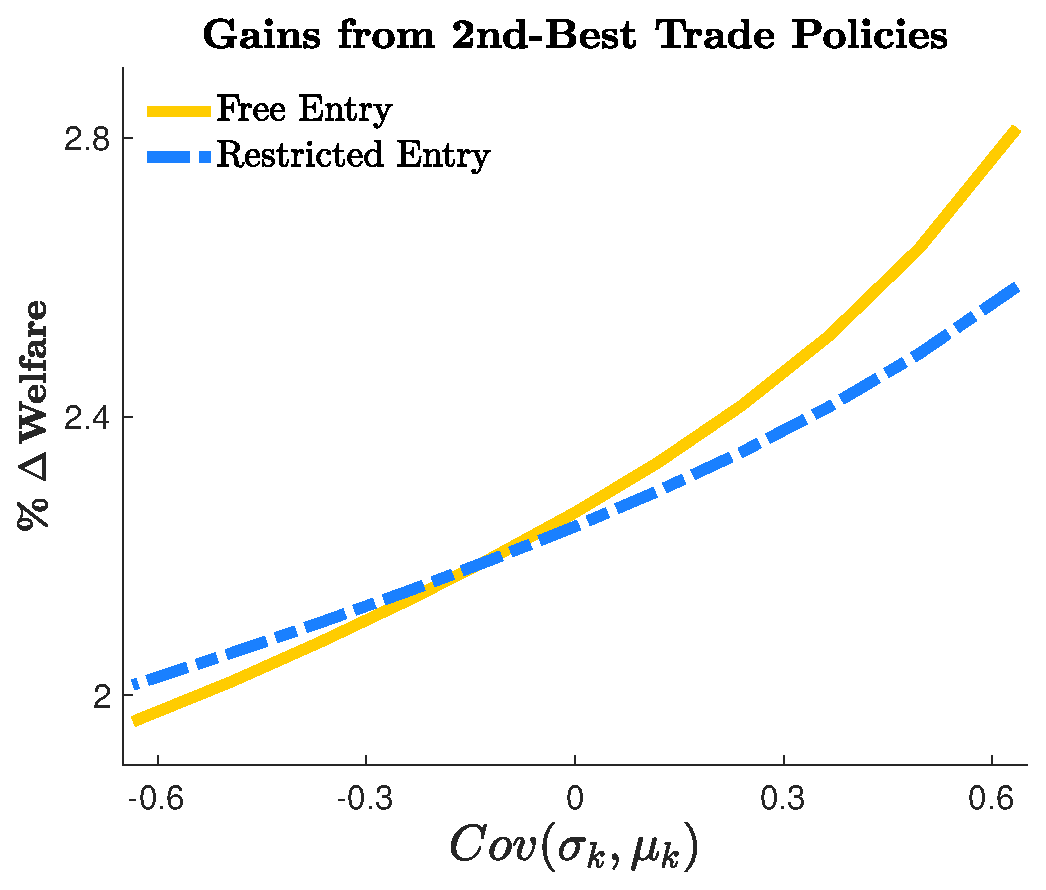
\includegraphics[scale=0.45]{matlab_output/Figure_1A}\hspace*{10pt}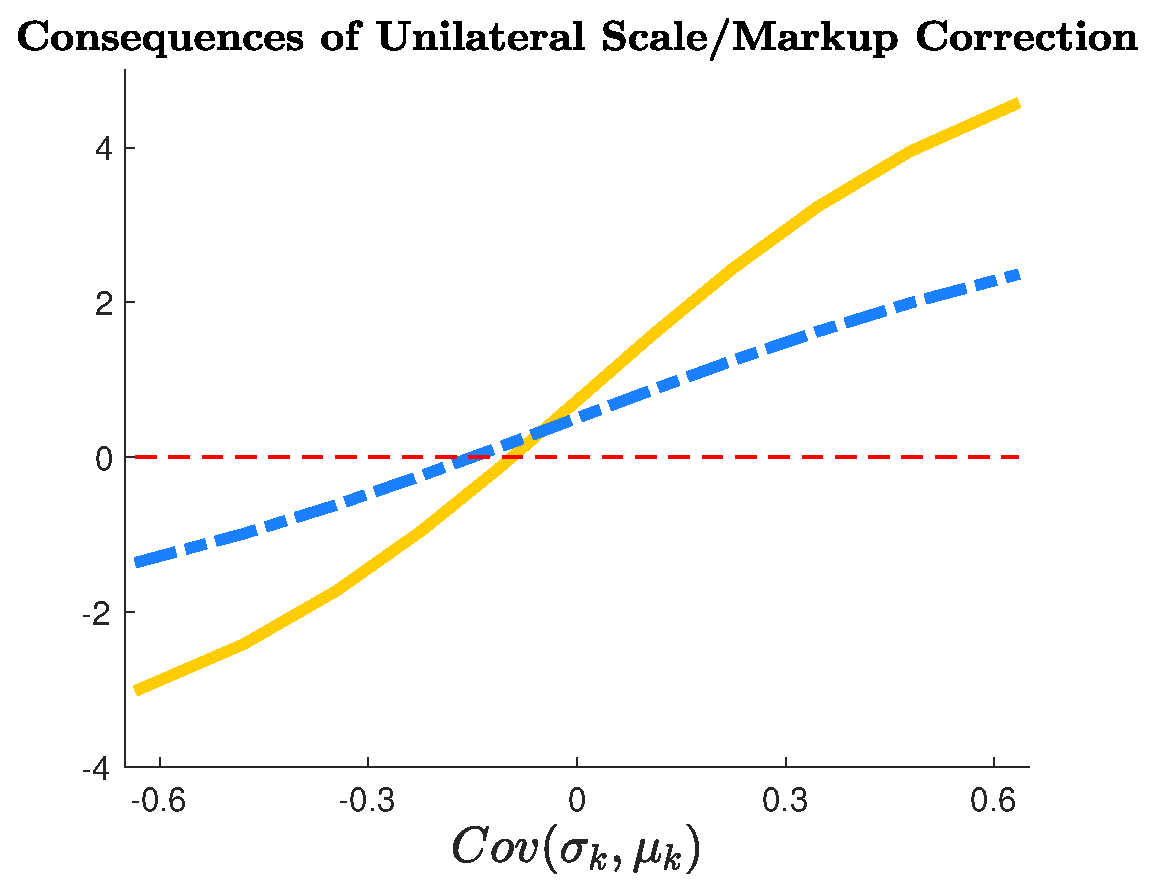
\includegraphics[scale=0.45]{matlab_output/Figure_1B}
\par\end{centering}
\emph{\small{}}%
\noindent\begin{minipage}[t]{1\columnwidth}%
\begin{spacing}{0.8}
\emph{\small{}Note}{\small{}: This figure corresponds to a two-country
and two-industry model with symmetric countries and Cobb-Douglas preferences
across industries. The left panel report the gains from Second-best
trade taxes, specified by Theorem 2. The trade elasticities in industries
1 and 2 are assigned values $\sigma_{1}=1.5$ and $\sigma_{2}=3$
and scale elasticities are adjusted to vary $Cov\left(\sigma_{k},\mu_{k}\right)$.
The right panel reports the welfare consequences of unilateral scale
or markup correction. Industry-level scale elasticities are assigned
values $\mu_{1}=0.5$ and $\mu_{2}=0.2$ and trade elasticities are
adjusted to vary $Cov\left(\sigma_{k},\mu_{k}\right)$.}
\end{spacing}
%
\end{minipage}\emph{\small{}}\\
{\small{}\vspace{-0.25in}}{\small\par}
\end{figure}
\emph{\medskip{}
}\\
\textbf{Unilateral Scale Correction can Cause Immiserizing Growth.}$\quad$

The flip side of the noted tension is that if $Cov\left(\sigma_{k},\mu_{k}\right)<0$,
unilateral implementation of scale-correcting Pigouvian subsidies
worsens the ToT, resulting in possibly adverse welfare consequences.
These arguments echo the \emph{immiserizing growth} paradox in \citealp{bhagwati1958immiserizing}
and follow a simple logic. If $Cov\left(\sigma_{k},\mu_{k}\right)<0$,
scale-correcting Pigouvian subsidies expand domestic output in high-$\sigma$
industries, which are nationally differentiated industries in which
countries hold significant export market power. Elevating output and,
thus, exports in these industries could worsen the ToT to the point
of triggering immiserizing welfare effects. 

Online Appendix \ref{sec: Proof-of-Propositions 1 =000026 2} demonstrates
theoretically that if $Cov\left(\sigma_{k},\mu_{k}\right)<0$, unilateral
scale/markup correction worsens the ToT. But whether these adverse
ToT effects outweigh the allocative efficiency gains from scale/markup
correction is an empirical matter. We conjecture that if industry-level
trade and scale elasticities exhibit a \emph{strong} negative correlation,
the adverse ToT effects from scale correction are large enough to
cause immiserizing growth. 
\begin{conjecture}
If industry-level trade and scale elasticities exhibit a strong negative
correlation ($\mbox{{Cov\ensuremath{\left(\sigma_{k},\mu_{k}\right)\ll}0}}$),
unilateral scale (or markup) correction via industrial policy will
likely worsen national welfare, echoing the immiserizing growth paradox.
\end{conjecture}
We evaluate this conjecture with micro-estimated parameters in Section
\ref{sec:Quantifying-the-Gains}, but a numerical illustration with
artificial parameter values is also provided in Figure \ref{fig: Tension}
(right panel). This figure is produced by fixing the degree of inter-industry
misallocation and artificially adjusting trade elasticities to vary
$Cov\left(\sigma_{k},\mu_{k}\right)$ from positive to negative values.
In regions where $Cov\left(\sigma_{k},\mu_{k}\right)<0$, a unilateral
adoption of scale-correcting subsidies compromises welfare, causing
immiserizing growth. These immiserizing consequences, as we discuss
next, can be an obstacle for industrial policy implementation for
countries committed to efficient trade policies under shallow agreements.\emph{\medskip{}
}\\
\textbf{Industrial Policy Coordination via Deep Agreements.}$\quad$Immizerising
growth can be a major obstacle to industrial policy implementation
in open economies. To convey this point, we adopt the common view
that intentional negotiations involve two stages.\footnote{Modeling international cooperation as a two-stage game consisting
of \emph{enactment} and \emph{implementation} stages is commonplace
in the global governance literature (\citet{shaffer2009hard}). In
the trade and environmental policy literature, many studies treat
international negotiations as multi-stage games where initial stages
restrict policy choices and latter stages ensure implementation (e.g.,
\citet{murdoch2003participation,drazen2008bargaining,kosfeld2009institution}).} In the first-stage, governments negotiate over policy space to ensure
each party restricts itself to the globally efficient policy choice
(Equation \ref{eq: deep cooperation}). In the second stage, governments
negotiate a deeper agreement to ensure the implementation of efficient
(misallocation-correcting) policies, with each country having the
choice to either implement efficient policies or withhold implementation.

Table \ref{tab: Coordination Game} illustrates the second-stage implementation
game facing cooperative countries. The game involves two cooperative
countries ($i$ and $j$) that can take two actions: $(1)$ implement
scale-correcting Pigouvian subsidies, \emph{i.e.}, $\textbf{s}_{i}=\boldsymbol{\mu}$,
or $(2)$ withhold implementation and stick to business as usual,
\emph{i.e.}, $\textbf{s}_{i}=\textbf{0}$. The efficient outcome is
the implementation of Pigouvian subsidies in both countries, which
will boost welfare by 2.7\% across the board. But this outcome is
not sustainable without formal coordination, because each country
has an incentive to free-ride on the other country's implementation.
The outcome of this game is a race to bottom, wherein no party is
willing to correct misallocation in domestic industries without violating
its commitments to shallow cooperation (i.e., zero trade taxes).\footnote{We must emphasize that a race to the bottom will not occur if $Cov(\sigma_{k},\mu_{k})\geq0$.
In that case, a unilateral adoption of corrective subsidies improves
rather than deteriorates the terms of trade, making unilateral implementation
a dominant strategy. We nevertheless maintain our focus on the case
where $Cov(\sigma_{k},\mu_{k})<0$ because it aligns with our forthcoming
estimation of scale and trade elasticities.} A deep agreement that ensures reciprocity in industrial policy implementation
can remedy this problem.

\begin{table}[!tbh]
\caption{\label{tab: Coordination Game}The industrial policy implementation
game facing cooperative governments when $Cov\left(\sigma_{k},\mu_{k}\right)<0$}

\begin{center}
\setlength{\extrarowheight}{4pt} 
\begin{tabular}{*{4}{c|}}      
\multicolumn{2}{c}{} & \multicolumn{2}{c}{Country $j$ (\%$\Delta W_j$)} \\
\cline{3-4}      
\multicolumn{1}{c}{} &  & $\textbf{s}_j=\textbf{0}$ & $\textbf{s}_j=\boldsymbol{\mu}$ \\
\cline{2-4}       \multirow{2}*{Country $i$ (\%$\Delta W_i)$}  & $\textbf{s}_i=\textbf{0}$ & $(\; 0\% \; , \; 0\% \;) $ & $(\; 3.7\% \; , \; -1.2\%\;)$ \\ 
\cline{2-4}       & $\textbf{s}_i=\boldsymbol{\mu}$ & $(\; -1.2\% \; , \; 3.7\% \;)$ & $(\; 2.7\% \; , \; 2.7\% \;)$ \\
\cline{2-4}     
\end{tabular} 
\end{center} \vspace{0.1in}

\begin{spacing}{0.8}
{\small{}}%
\noindent\begin{minipage}[t]{1\columnwidth}%
\begin{spacing}{0.8}
\emph{\small{}Note}{\small{}: This figure corresponds to a two-country
and two-industry model with symmetric countries and CES preferences
across industries with substitution elasticity $1.2$. Industry-level
level trade elasticities are $\sigma_{1}=1.5$ and $\sigma_{2}=3$
and scale elasticities are $\mu_{1}=0.2$ and $\mu_{2}=0.5$, implying
$Cov\left(\sigma_{k},\mu_{k}\right)\approx-0.225$. The unique Nash
equilibrium is a race to the bottom, wherein $\textbf{s}_{i}=\textbf{s}_{j}=\textbf{0}$.}
\end{spacing}
%
\end{minipage}{\small\par}
\end{spacing}
\end{table}

In principle, the first-mover country can renegotiate their tariffs
to nullify the adverse ToT effects of unilateral scale correction---for
example, under Article XXVIII of the GATT. But these negotiations
are costly, suggesting that governments might prefer to refrain from
implementation and opt for free-riding. Alternatively, countries may
pair their industrial policy with \emph{hidden} trade restrictions,
enabling them to avoid adverse ToT effects without incurring the administrative
cost of tariff renegotiation. The Chinese government, for instance,
has coupled its proactive industrial policy measures with hidden export
taxes, which are applied via partial value-added tax rebates and enhance
China's terms of trade (\citet{garred2018persistence}).

\section{\label{sec: Extensions}Extensions and Application to other Canonical
Models}

In this section, we first show that our theoretical results readily
apply to two other canonical trade models. We then extend our baseline
theoretical results to richer environments featuring input-output
linkages and political economy pressures.

\subsection{Application to Other Canonical Trade Models}

The optimal policy formulas specified by Theorems 1-3 apply to two
other canonical trade models. Though, parameters $\sigma_{k}$ and
$\mu_{k}$ in these formulas adopt different interpretations, which
reflects the different micro-foundation underlying these frameworks.\medskip{}

\emph{The Eaton-Kortum model with Marshallian externalities.$\quad$}Consider
a multi-industry \citet{Eaton2002} model where industry-level production
is subject to agglomeration economies. Let $\psi_{k}$ denote the
constant agglomeration elasticity in industry $k$, and $\theta_{k}$
denote the Eaton-Kortum Fr�chet shape parameter. Theorem 1 characterizes
the optimal policy in this model under the following reinterpretation
of parameters: $\mu{}_{k}^{\textrm{EK}}=\psi_{k}$ and $\sigma_{k}^{\textrm{EK}}=1+\theta_{k}$.
The tension between the \emph{ToT }and \emph{allocative efficiency}
manifests itself in this model if $Cov(\psi_{k},\theta_{k})<0$. The
fact that our theory readily extends to the Eaton-Kortum model echoes
the isomorphism established in \citet{kucheryavyy2023grounded}. Online
Appendix \ref{sec: Nested-EK} shows that this isomorphism is even
more profound. The nested-CES import demand function implied by (A1),
we demonstrate, may analogously arise from within-industry specialization
\'a la Eaton-Kortum.\medskip{}

\emph{The Melitz-Pareto model.$\quad$}Consider a multi-industry \citet{Melitz2003}
model that features the same nested-CES demand function specified
by (A1). Suppose the firm-level productivity distribution is Pareto
in each industry with a shape parameter, $\vartheta_{k}$. Online
Appendix \ref{sec: Appendix Firm-Selection} establishes that the
Melitz-Pareto model is isomorphic to our baseline Krugman model insofar
as macro-level representation is concerned. Hence, Theorem 1 characterizes
the optimal policy in the Melitz-Pareto model under the following
reinterpretation of parameters: $\mu_{k}^{\textrm{Melitz}}=\frac{\gamma_{k}\vartheta_{k}}{\left(\gamma_{k}-1\right)\left(\vartheta_{k}+1\right)-\vartheta_{k}}-1$
if entry is restricted and $\mu_{k}^{\textrm{Melitz}}=\frac{1}{\vartheta_{k}}$
if entry is free; and $\sigma_{k}^{\textrm{Melitz}}=1+\vartheta_{k}\left[1+\vartheta_{k}\left(\frac{1}{\sigma_{k}-1}-\frac{1}{\gamma_{k}-1}\right)\right]^{-1}$.
This mapping indicates that we need to estimate parameter $\vartheta_{k}$,
in addition to $\sigma_{k}$ and $\gamma_{k}$, to quantify the gains
from policy under firm-selection effects---a procedure we formally
undertake and elaborate on in Section \ref{sec:Quantifying-the-Gains}. 

\subsection{Extension \#1:\emph{ }Accounting for Input-Output Networks}

Suppose production employs both labor and intermediate inputs, which
are distinguished from final goods by superscript $\mathcal{I}$.
Cost minimization entails that the producer price of good $ij,k$
(origin $i$--destination $j$--industry $k$) depends on $(i)$
the wage rate in origin $i$ and $(ii)$ the price of all intermediate
inputs, $\tilde{\textbf{P}}_{i}^{\mathcal{I}}\equiv\{\tilde{P}_{nj,k}^{\mathcal{I}}\}$,
available to firms in origin $i$. Namely,
\begin{equation}
P_{ij,k}=\bar{\rho}_{ij,k}\textrm{C}_{i,k}(w_{i},\tilde{\textbf{P}}_{i}^{\mathcal{I}})\mathcal{Q}_{i,k}^{-\frac{\mu_{k}}{1+\mu_{k}}},\label{eq: Producer Price (IO)}
\end{equation}
where $\textrm{C}_{i,k}(.)$ is a homogeneous of degree one function
w.r.t. $w_{i}$ and $\tilde{\textbf{P}}_{i}^{\mathcal{I}}$.\footnote{Without loss of generality, we assume that good $ji,k$ can be used
as either an intermediate input or a final consumption good, with
taxes being applied on a good irrespective of the intended final use,
i.e., $\tilde{P}_{ij,k}^{\mathcal{I}}=\tilde{P}_{ij,k}$. This assumption
is innocuous, because we can fragment every industry $k$ into a final
good version $k'$ and an intermediate good version $k''$. Since
we do not impose any restrictions on the number of industries, our
theory extends to the case where differential taxes are imposed on
fragments $k'$ and $k''$.} The dependence of $P_{ij,k}$ on gross industry-level output, $\mathcal{Q}_{i,k}\equiv\sum_{j\in\mathbb{C}}\left[\bar{a}_{ij,k}Q_{ij,k}\right]$,
reflects scale economies under free entry. The formal definition of
general equilibrium under input-output (IO) linkages is presented
in online Appendix \ref{sec: Extended Optimal-Tax-Formula}. The same
appendix characterizes optimal policy using an augmented version of
our dual approach that leverages additional supply-side envelope conditions.
Our characterization reveals that the formulas for optimal industrial
subsidies and import tariffs are IO-blind---\emph{i.e.}, they are
similar to Theorem 1. There is a simple intuition for this result:
Although a tariff on imported inputs can influence prices in the rest
of the world through re-exportation, any potential ToT gains from
tariff re-exportation are already internalized by the government's
optimal choice vis-\`a-vis export tax-cum-subsidies. Consistent with
this intuition, the optimal export subsidy formula features an explicit
adjustment for export subsidy reimportation via the IO network. The
following theorem formalizes these results.
\begin{theorem}
Under IO linkages, the unilaterally first-best import tariffs and
domestic subsidies are IO-blind; but 1st-best export subsidies exhibit
an upward-adjustment that account for re-importation via the IO network.
More formally, the unilaterally first-best policy schedule is given
by\emph{
\begin{align*}
\hspace{-0.25in}[\text{domestic subsidy}]\ \ \ \ \ \ \ \ \ \ \ \ 1+s_{i,k}^{*} & =\left(1+\mu_{k}\right)(1+\bar{s}_{i}^{\mathscr{C}})^{-1}\\
\hspace{-0.25in}[\text{import tax}]\ \ \ \ \ \ \ \ \ \ \ \ 1+t_{ji,k}^{*} & =(1+\omega_{ji,k})\left(1+\bar{t}_{i}\right)(1+\bar{s}_{i}^{\mathscr{C}})\\
\hspace{-0.25in}[\text{export subsidy}]\ \ \ \ \ \ \ \ \ \ \ \ \textbf{1}+\textbf{x}_{ij}^{*} & =-\textbf{E}_{ij}^{-1}\left[\textbf{E}_{ij}^{(-ij)}\left(\textbf{1}+\textbf{t}_{i}^{*}\right)+\boldsymbol{\Lambda}_{ij}(1+\bar{t}_{i})(1+\bar{s}_{i}^{\mathscr{C}})\right],
\end{align*}
}where elements of $\boldsymbol{\Lambda}_{ij}\equiv\left[\Lambda_{ij,k}\right]_{k}$
correspond to the fraction of good $ij,k$ that is reimported, and
$\bar{s}_{i}^{\mathscr{C}}$is an arbitrary tax shifter that assumes
a positive value if the taxed item is a final good and zero otherwise.\footnote{If country $i$ is a small open economy, $\Lambda_{ij,k}\approx\boldsymbol{0}$.
Correspondingly, optimal policy formulas for a small open economy
under IO linkages perfectly overlap with the baseline formulas specified
under Equation \ref{eq: small open economy}. } 
\end{theorem}
The above theorem indicates that the tax-equivalent of export subsidies
is relatively lower on intermediate inputs to mitigate export tax-reimportation
via the IO network.\footnote{In the absence of scale economies or profits, $\omega_{ji,k}=0$.
So, Theorem 1 posits that optimal import tariffs are uniform by choice
of $\bar{s}_{i}^{\mathscr{C}}=0$ in the multi-industry Armington
and Eaton--Kortum models (see online Appendix \ref{sec: Simple IO}).} Moreover, there is a uniform wedge between final and intermediate
input taxes as represented by the final good tax-shifter, $\bar{s}_{i}^{\mathscr{C}}$.\footnote{Theorem 4 indicates that uniform markup pricing is not a necessary
condition for efficiency. Consider, for instance, a vertical production
economy where goods are used as either final goods or intermediate
inputs, but not both. The efficient policy, in this setup, must restore
uniform markup pricing within input and final good segments but not
across---see \citet{antras2022trade} for further exploration of
this issue.} This detail aside, the ToT-improving motive for policy still requires
export contraction in low-$\sigma$ industries, while the misallocation-correcting
objective asks for output expansion in high-$\mu$ industries. So,
unless intermediate inputs exhibit a systemically lower $\sigma$,
our conjecture about the inefficacy of standalone trade policy measures
withstands.\footnote{Theorem 4 offers insight into the structure of second-best import
tariffs and export subsidies under IO linkages. Several papers, including
\citet{blanchard2016global}, \citet{beshkar2020cost}, \citet{caliendo2021second},
and \citet{antras2022trade}, examine in more detail how IO linkages
impact 3rd-best import tariff choices. \citet{beshkar2020cost}, moreover,
adopt a special case of Theorem 4, with Cobb-Douglas production and
no scale economies, to examine the cost of trade wars.} 

\subsection{Extension \#2:\emph{ }Accounting for Political Economy Pressures}

Suppose optimal policy choices internalize political economy pressures
\`a la \citeauthor{ossa2014trade}'s \citeyearpar{ossa2014trade}
adaptation of \citet{grossman1994protection}. That is, the government
maximizes a politically-weighted welfare function, $W_{i}\equiv V_{i}(w_{i}L_{i}+\mathcal{R}_{i}+\sum_{k}\pi_{i,k}\Pi_{i,k},\tilde{\textbf{P}}_{i})$,
where $\pi_{i,k}$ is the political economy weight assigned to industry
$k$'s profits (with $\sum_{k}\pi_{i,k}/K=$1). It follows trivially
from Theorem 1 that the first-best policy in the political setup consists
of the same trade tax/subsidy formulas but a politically-adjusted
industrial subsidy rate. Namely,
\begin{align*}
1+s_{i,k}^{*} & =(1+\mu_{i,k}^{\mathscr{P}})\left(1+\bar{s}_{i}\right),
\end{align*}
where $\mu_{i,k}^{\mathscr{P}}=\frac{\mu_{k}}{\pi_{i,k}-(1-\pi_{i,k})\mu_{k}}$
is the \emph{political economy-adjusted} markup of industry $k$.
Considering the above formulas: if $Cov\left(\pi_{i,k},\mu_{k}\right)<0$,
the optimal policy may tax high-$\mu$ industries to the detriment
of social welfare. In that case, even if $Cov(\sigma_{k},\mu_{k})>0$,
the misallocation-correcting and ToT motives for trade taxation will
clash. However, if $Cov\left(\pi_{i,k},\mu_{k}\right)\geq0$, our
conjecture about the inefficacy of standalone trade policy measures
withstands.

\section{\label{sec:Estimation}Estimating the Key Policy Parameters}

Based on our theory, policy evaluation in open economies requires
credible estimates for industry-level \emph{trade elasticities}, $\sigma_{k}$,
and industry-level \emph{scale elasticities}, $\mu_{k}\sim\frac{1}{\gamma_{k}-1}$.
The former governs the degree of national-level market power, while
the latter regulates the extent of love-for-variety. The trade literature
has paid considerable attention to estimating $\sigma_{k}$, but less
to estimating $\mu_{k}$. The existing policy literature typically
normalizes $\mu_{k}$ in one of two ways: $(i)$ $\mu_{k}=\frac{1}{\sigma_{k}-1}$
in imperfectly competitive models, and $(ii)$ $\mu_{k}=0$ in perfectly
competitive models.\footnote{See \citet{ossa2016quantitative} and \citet{costinot2014trade} for
a synthesis of the previous literature. Under restricted entry, $\mu_{k}$
denotes the firm-level markup, which can be alternatively estimated
with firm-level production data (e.g., \citet{de2012markups}, \citet{deloecker16}).} Both normalizations impose artificial restrictions on $Cov\left(\mu_{k},\sigma_{k}\right)$,
which following the discussion in Section \ref{sec: Tension}, can
bias the estimated gains from policy. 

Against this backdrop, we seek to estimate $\sigma_{k}$ and $\mu_{k}$
in a way that ascertains mutual consistency, giving us a credible
assessment of $Cov\left(\mu_{k},\sigma_{k}\right)$. To this end,
we propose a new methodology that simultaneously estimates $\sigma_{k}$
and $\mu_{k}$ from the same data.\footnote{In the presence of firm-selection effects, our estimated parameters
are necessary but not sufficient to pin down the trade and scale elasticities---see
online Appendixes \ref{sec: Appendix Firm-Selection} and \ref{sec: Gains Robustness}
for details. } Our approach involves fitting the structural \emph{firm-level} import
demand function implied by A1 to the universe of Colombian import
transactions from 2007--2013. We outline this approach below, starting
with a description of the data used in our estimation.\emph{\medskip{}
}\\
\textbf{Data Description.}$\quad$Our estimation uses data on import
transactions from the Colombian Customs Office during 2007--2013.\footnote{The data is obtained from \noun{Datamyne}, a company that specializes
in documenting import and export transactions in Americas. For more
detail, please see \url{www.datamyne.com}. Our estimation also employs
data on monthly average exchange rates, which are taken from the Bank
of Canada: \url{http://www.bankofcanada.ca/rates/exchange/monthly-average-lookup/}.
A detailed description of all the datasets used in this paper is provided
in online Appendix \ref{sec:Data-Appendix}.} The data include detailed information about each transaction, such
as the Harmonized System 10-digit product category (HS10), country
of origin, importing and exporting firm IDs, quantity, f.o.b. (free
on board), and c.i.f. (customs, insurance, and freight) transaction
values, freight, insurance, and value-added tax in US dollars. As
a unique feature, our data reports the identities of all foreign firms
exporting to Colombia. This feature allows us to define import varieties
as firm-product combinations rather than country-product combinations,
which is the standard approach. Table \ref{tab:Summary Statistics}
(in the online appendix) reports a summary of basic trade statistics
in our data. Working with firm-level data presents two challenges:
First, exporters are not identified by unique standardized IDs. Instead,
they are identified by a name, a number, and an address. We handle
this problem by standardizing the spelling and lengths of firms' names
and using the information on firms' phone numbers (see online Appendix
\ref{sec:Data-Appendix}). Second, Colombia changed the HS10 classification
for some products between 2007 and 2013. Fortunately, the Colombian
Statistical Agency, DANE, keeps track of these changes. We utilize
this information to concord the Colombian HS10 codes over time, using
the guidelines in \citet{Pierce_Schott}. Overall, changes in HS10
codes between 2007 and 2013 affect less than 0.1\% of our data points.

\subsection{Estimating Equation}

Since we are focusing on one importer, we hereafter drop the importer's
subscript $i$ and add a year subscript $t$ to account for the time
dimension of our data. With this switch in notation, the demand facing
firm $\omega$ located in country $j$ and supplying product $k$
in year $t$ is given by:
\begin{equation}
q_{j,kt}\left(\omega\right)=\varphi_{j,kt}(\omega)\left(\frac{\tilde{{p}}_{j,kt}(\omega)}{\tilde{P}_{j,kt}}\right)^{-\gamma_{k}}\left(\frac{\tilde{P}_{j,kt}}{\tilde{P}_{kt}}\right)^{-\sigma_{k}}Q_{kt},\label{eq: Import Demand Function}
\end{equation}
Subscript $k$, in our theoretical model, designated industries. In
our estimation, $k$ denotes an HS10 product---the most disaggregated
product classification in our data. The quadruplet ``$\omega jkt$''
accordingly denotes a unique variety corresponding to \emph{firm $\omega$--country
of origin $j$--HS10 product $k$--year $t$}. Let $\tilde{x}(\omega)\equiv\tilde{p}(\omega)q(\omega)$
denote gross sales. Rearranging Equation \ref{eq: Import Demand Function}
yields the following log-linear import demand function facing individual
varieties:
\begin{equation}
\ln\tilde{x}_{j,kt}(\omega)=\left(1-\sigma_{k}\right)\ln\tilde{p}_{j,kt}(\omega)+\left(1-\frac{\sigma_{k}-1}{\gamma_{k}-1}\right)\ln\lambda_{j,kt}\left(\omega\right)+D_{kt}+\ln\varphi_{j,kt}(\omega),\label{eq: Estimated Equation Final}
\end{equation}
where $D_{kt}\equiv\ln P_{kt}^{\sigma_{k}}Q_{kt}$ can be treated
as a product-year fixed effect and $\lambda_{j,kt}\left(\omega\right)$
denotes the share of expenditure on firm $\omega$ \emph{conditional}
on buying good $k$ from country of origin $j$,
\[
\lambda_{j,kt}\left(\omega\right)\equiv\varphi_{j,kt}(\omega)\left(\frac{\tilde{{p}}_{j,kt}(\omega)}{\tilde{P}_{j,kt}}\right)^{1-\gamma{}_{k}}=\frac{\tilde{x}_{j,kt}\left(\omega\right)}{\sum_{\omega'\in\Omega_{j,kt}}\tilde{x}_{j,kt}\left(\omega\right)}.
\]
We assume that $\varphi_{jkt}(\omega)=\bar{\varphi}_{j,k}(\omega)\times\varphi_{\omega jkt}$
can be decomposed into a time-invariant \emph{firm-and-product}-specific
quality component, $\bar{\varphi}_{j,k}(\omega)$, and a time-varying
component $\varphi_{\omega jkt}$, that encompasses idiosyncratic
variations in consumer taste, measurement errors, and/or omitted variables
that account for dynamic demand optimization. To eliminate $\bar{\varphi}_{j,k}(\omega)$
from the estimating equation, we employ a first-difference estimator,
which also drops observations pertaining to one-time exporters. We
deem the first-difference estimator appropriate given the possibility
that $\varphi_{\omega jkt}$'s are sequentially correlated. As a robustness
check, we also report estimation results based on a two-way fixed
effects estimator in online Appendix \ref{sec: Two-Ways FE Estimation}.\footnote{Following \citet{boehm2020long}, the first-difference estimation
offers a partial remedy for omitted variable bias and reverse causality.
Both issues pose a serious challenge to traditional log-level estimations
of import demand. Depending on the application, though, the first-difference
estimator may not necessarily identify the desired long-run elasticity.
As detailed in online Appendix \ref{sec: Two-Ways FE Estimation},
this limitation is less severe in our firm-level estimation---as
we explicitly control for the extensive margin of trade. We illustrate
this point formally in online Appendix \ref{sec: Two-Ways FE Estimation}
by re-estimating Equation \ref{eq: Estimated Equation Final} in levels
and comparing the estimation results to the baseline values. } Stated in terms of first-differences, our estimating equation takes
the following form
\begin{equation}
\Delta\ln\tilde{x}_{j,kt}(\omega)=\left(1-\sigma_{k}\right)\Delta\ln\tilde{p}{}_{j,kt}\left(\omega\right)+\left(1-\frac{\sigma_{k}-1}{\gamma_{k}-1}\right)\Delta\ln\lambda_{j,kt}\left(\omega\right)+\Delta D_{kt}+\Delta\ln\varphi{}_{\omega jkt},\label{eq:Main}
\end{equation}
where $\Delta\ln\varphi_{\omega jkt}$, roughly speaking, represents
a variety-specific demand shock; and $\Delta D_{kt}$ is a product-year
fixed effect.\footnote{To handle outliers, we trims our sample to exclude observations that
report a price change, $\Delta\ln\tilde{p}{}_{j,kt}\left(\omega\right)$,
above the 99th percentile or below the 1st percentile of the HS10
product code $k$ in year $t$.} Of the remaining variables, $\Delta\ln\tilde{p}_{j,kt}(\omega)$
and $\Delta\ln\tilde{x}_{j,kt}(\omega)$ are directly observable for
each import variety. The change in the \emph{within-national} market
share, $\Delta\ln\lambda_{j,kt}\left(\omega\right)$, can be calculated
using the universe of firm-level sales to Colombia.\\

\medskip{}
\emph{Recovering Scale \& Trade Elasticities from Demand Parameters.$\quad$}Equation
\ref{eq:Main} allows us to estimate demand parameters, $\sigma_{k}$
and $\gamma_{k}$, from which we can recover the scale and trade elasticities
as follows (see Section \ref{sec:Theoretical-Framework} for the underlying
theoretical foundation):
\[
\mu_{k}=\frac{1}{\gamma_{k}-1}\sim\text{scale elasticity}\qquad\qquad\qquad\text{\ensuremath{\sigma_{k}}}\sim\text{trade elasticity}
\]
The reason we can infer $\mu_{k}$ from demand parameters is that
the scale elasticity in the generalized \citeauthor{Krugman1980}
model reflects the extent of \emph{love-for-variety}---the social
benefits of which are not internalized by firms' entry decisions.
In the \citeauthor{Melitz2003}-Pareto case, we also need estimates
for the shape of the Pareto productivity distribution (in addition
to $\gamma_{k}$ and $\sigma_{k}$) to recover the scale elasticity---see
online Appendix \ref{sec: Robustness-Checks}. Our estimation is,
of course, unable to detect scale externalities unrelated to love-for-variety.
These externalities can be estimated using techniques that leverage
scale-related moments, but under stronger assumptions about the variability
of production inputs. We discuss the relative advantages of each technique
in online Appendix \ref{sec: Overview-of-Scale-Estimation}.\footnote{In the restricted entry case, our demand estimation identifies the
firm-level markup in each industry. Following an old tradition in
the industrial organization literature, we assume that market conduct
is monopolistic competition and recover firm-level markups as $\mu_{k}=\frac{1}{\gamma_{k}-1}$.
Online Appendix \ref{sec: Appendix Tension} recovers markups under
alternative market conduct assumptions.}\\

\medskip{}
\emph{Breaking the Sample into Broadly-Defined Industries.$\quad$}As
noted earlier, $k$ indexes an HS10 product category in Equation \ref{eq:Main}.
To conduct our forthcoming quantitative analysis, we must estimate
demand parameters for 14 broadly-defined industries based on the World
Input-Output Database (WIOD) industry classification. Considering
this, we pool all HS10 products belonging to the same WIOD industry
$\mathcal{K}$ together and estimate Equation \ref{eq:Main} on this
pooled sample assuming that $\sigma_{k}$ and $\gamma_{k}$ are uniform
across products within the same industry (i.e., $\gamma_{k}=\gamma_{\mathcal{K}}$
and $\sigma_{k}=\sigma_{\mathcal{K}}$ for all $k\in\mathbb{K}_{\mathcal{K}}$).
In principle, we can also estimate the import demand function separately
for each HS10 product category to attain HS10-level elasticities.
However, such elasticities will be of little use for quantitative
policy analysis, as multi-country data on trade, production, and expenditure
shares are scarce at such levels of disaggregation.

\subsection{Identification Strategy}

The identification challenge we face is that $\Delta\ln\tilde{p}{}_{j,kt}\left(\omega\right)$
and $\Delta\ln\lambda_{j,kt}\left(\omega\right)$ are endogenous variables
that can covary with the demand shock, $\Delta\ln\varphi{}_{\omega jkt}$.\footnote{Another challenge is that unit price data may be contaminated with
measurement errors, as they are averaged across many transactions.
Following \citet{Berry1994}, this type of measurement error is fairly
innocuous when dealing with log-linear demand functions. Furthermore,
our instrumental variable approach will handle measurement errors,
provided that lagged monthly sales patterns are uncorrelated with
concurrent measurement errors.} Traditional \emph{country-level} import demand estimations overcome
a similar challenge by instrumenting for prices with plausibly exogenous
tariff rates.\footnote{A prominent example is \citet{caliendo2014estimates}, who use tariff
data to identify the trade elasticity. } This strategy, however, does not suit our \emph{firm-level} estimation
because tariffs discriminate by country-of-origin but not across firms
from the same country.

We employ a shift-share research design to overcome our \emph{firm-level}
identification challenge. Our approach is rooted in two data observations:
First, a typical variety is imported under multiple invoices spread
across different months in a given year. As a matter of accounting,
the annual-level price of a variety is the quantity-weighted average
of monthly prices. Namely, $p_{j,kt}\left(\omega\right)=\sum_{m\in\mathcal{M}}\tilde{s}_{j,kt}(\omega;m)p_{j,kt}\left(\omega;m\right)$,
where $m$ denotes month and $\tilde{s}\left(\omega;m\right)$ and
$p\left(\omega;m\right)$ denote the quantity share and price associated
with month $m$. Second, the month $m$ price of an imported variety
(in Colombian Pesos) is equal to \emph{markup-plus-taxe}s$\times$\emph{marginal
input cost invoiced in local currency$\times$exchange rate in month
$m$. }More formally, $p_{j,kt}\left(\omega;m\right)=\tau_{j,kt}\left(\omega\right)\times\text{C}_{j,kt}\left(\omega\right)\times\mathcal{E}_{jt}(m)$,
where $\tau$ and $\text{C}$ respectively denote markup-plus-tax
and marginal cost, while $\mathcal{E}_{jt}(m)$ represents the exchange
rate between origin $j$'s currency and the Colombian Peso in month
$m$ of year $t$. To a first-order approximation, the annual change
in variety-level prices in response to monthly exchange rate fluctuations
can be specified as
\[
\Delta\ln\tilde{p}{}_{j,kt}\left(\omega\right)\approx\sum_{m\in\mathcal{M}}s_{j,kt}(\omega;m)\,\Delta\ln\mathcal{E}_{jt}(m),
\]
where $\Delta\ln\mathcal{E}_{jt}(m)$ denotes the year-over-year change
in origin $j$'s exchange rate with the Colombian Peso in month $m$
; and $s_{j,kt}(\omega;m)$ is the share of month $m$ in variety
$\omega jkt$'s annual export sales to Colombia:
\[
s_{j,kt}\left(\omega;m\right)=\frac{\tilde{x}_{j,kt}(\omega;m)}{\sum_{m'\in\mathcal{M}}\tilde{x}_{j,kt}(\omega;m')}\,\sim\,\text{share of month \ensuremath{m} in annual export sales}
\]
Capitalizing on the above observation, we construct our shift-share
instrument as the inner product of \emph{lagged} monthly export shares
and monthly exchange rate changes. Namely,
\[
z_{j,kt}(\omega)=\sum_{m\in\mathcal{M}}s_{j,kt-1}\left(\omega,m\right)\Delta\ln\mathcal{E}_{jt}\left(m\right).
\]
Stated verbally, $z_{j,kt}(\omega)$ measures exposure to exchange
rate fluctuations at the \emph{firm$\times$origin$\times$product$\times$year}
level. The idea being that aggregate exchange rate movements have
differential effects on individual firms depending on the monthly
composition of their prior export activity to Colombia.\footnote{Leveraging exchange rate data to construct firm-level input cost shifters
has been also explored by \citet{piveteau2019estimating} and \citet{amiti2019international}.} Encouragingly, the validity of our instrument is corroborated by
the strong and statistically significant correlation between $z$
and $\Delta\ln\tilde{p}$. Online Appendix \ref{sec:Illustrative-Example}
illustrates this relationship visually using two U.S.-based firms
as an example.\medskip{}

\emph{Exclusion Restriction.}$\quad$Our instrument utilizes lagged
export shares, which depend on lagged prices and a set of market-level
indexes---namely, $s_{jkt-1}(\omega,m)=s(\tilde{p}_{jkt-1}(\omega,m);...)$.
Considering this, the exclusion restriction in our setup, $\mathbb{E}\left[z\,\Delta\ln\varphi\right]=0$,
rests on two conditions:
\begin{lyxlist}{00.00.0000}
\item [{(C1)}] Prior price-setting decisions (and thus lagged export shares)
are orthogonal to concurrent demand shocks: $\mathbb{E}\left[\tilde{p}_{j,kt-1}(\omega)\,\Delta\ln\varphi_{\omega jkt}\right]=0$.
\item [{(C2)}] Monthly national-level exchange rate shocks are orthogonal
to variety-level demand shocks: $\mathbb{E}\left[\Delta\ln\mathcal{E}_{jt}(m)\,\Delta\ln\varphi_{\omega jkt}\right]=0$.
\end{lyxlist}
Since our sample features many firms and a finite number of months,
Condition (C1) is sufficient for the consistency of our estimates
(see Proposition 2.1 in \citealp{goldsmith2020bartik}). In fact,
our two-stage least squares (2SLS) estimator is numerically equivalent
to a generalized method of moments (GMM) estimator with lagged monthly
export shares as instruments and a weight matrix constructed from
monthly aggregate exchange rate shocks. Condition (C2), meanwhile,
is more crucial for the finite sample properties of our estimator.
Both conditions can, in principle, be violated if there are cross-inventory
linkages or if individual export varieties account for a significant
fraction of national exports to Colombia. We discuss and address these
issues in Section \ref{subsec: Discussion of Estimation}.\medskip{}

\emph{Instruments for $\Delta\ln\lambda_{j,kt}\left(\omega\right)$.}$\quad$Following
\citet{Khandelwal2010}, we construct two standard instruments for
the annual variation in the within-national market shares: \emph{$(i)$}
annual changes in the total number of origin $j$ firms serving the
Colombian market in product category $k$, and \emph{$(ii)$} changes
in the total number of HS10 product categories actively served by
firm $\omega$ in year $t$. These count measures will be correlated
with $\Delta\ln\lambda_{j,kt}\left(\omega\right)$ but uncorrelated
with $\Delta\ln\varphi_{\omega jkt}$ if variety-level entry and exit
occurs prior to, or independent of, the demand shock realization of
competing varieties. As noted by \citet{Khandelwal2010}, this assumption
is widely-invoked when estimating discrete choice demands curves---see
also \citet{Berry1995}.\footnote{Border taxes tend to be a weak instrument for firm-level prices in
our sample, but we include to comply with the past literature. These
include applied ad-valorem tariffs and the Columbian value-added tax
(VAT). We exclude the VAT component in the 'Transportation' and 'Petroleum'
industries since the VAT in these industries discriminates by the
delivery method and level of luxury---both of which may be correlated
with $\Delta\ln\varphi_{\omega jkt}$.}

\subsection{Estimation Results}

Table \ref{tab: Estimation result by sector} reports our industry-level
estimation results. We also report results corresponding to a pooled
sample of all industries in Table \ref{tab:Estimation results} of
the online appendix. The same table compares the 2SLS and OLS estimates
to ensure that our IV strategy operates in the expected direction.
Our estimates point to a median trade elasticity of $\sigma-1=3.9$
and a median scale elasticity of $\mu\approx0.20$. Our pooled estimation
yields a heteroskedasticity-robust Kleibergen-Paap Wald rk F-statistic
of $259$, rejecting the null of weak instruments given the Stock-Yogo
critical values. A similar albeit weaker outcome emerges from the
industry-level estimation.

The industry-level elasticities reported in Table \ref{tab: Estimation result by sector}
display considerable variation across industries. The estimated scale
elasticity or markup margin is highest in the 'Electrical \& Optical
Equipment' ($\mu=0.55$) and 'Petroleum' ($\mu=1.2$) industries;
both of which are associated with high R\&D or fixed costs. The estimated
scale elasticity is lowest in 'Agricultural \& Mining' ($\mu=0.14)$
and 'Machinery' ($\mu=0.12$) industries. Furthermore, with the exception
of 'Agriculture \& Mining,' we cannot reject the prevalence of scale
economies due to \emph{love-for-variety}.\footnote{The finding that returns-to-scale are negligible in the agricultural
sector aligns with a large body of evidence on the inverse farm-size
productivity (IFSP) relationship---see \citet{sen1962aspect} and
subsequent references to IFSP. }

Importantly, our estimates indicate that $\frac{\sigma_{k}-1}{\gamma_{k}-1}\neq1$
in nearly all industries. This finding rejects the arbitrary link
often assumed between the firm-level and national-level degrees of
market power in the literature. Our estimates also indicate that{\large{}
\[
Cov(\sigma_{k},\mu_{k})\,\approx\,-0.65,
\]
}which corroborates the innate tension between the \emph{ToT-improving}
and \emph{misallocation-correcting} objectives at the core of Conjectures
1 and 2.\footnote{Our trade elasticity estimates are one of the few based on firm-level
data. Traditional estimates of $\sigma_{k}$ are typically based on
country-level data (e.g., \citet{simonovska2014elasticity}; \citet{caliendo2014estimates}).}

\begin{table}[!tbh]
\caption{\label{tab: Estimation result by sector} Industry-level estimation
results}

\begin{adjustwidth}{-0in}{-0in}
\begin{tabular}{lccccccccccc}
                            \toprule
                          &           & &      \multicolumn{5}{c}{Estimated Parameter}                   && \phantom{abc}  & \phantom{abc} &        \\
                                                     \cmidrule{4-8}       
Sector 
& ISIC4 codes &&  $\sigma_{k}-1$ && $\frac{\sigma_{k}-1}{\gamma_{k}-1}$   && $\mu_{k}$ && Obs. &   \specialcell{\footnotesize Weak \\ Ident. Test} \\ 
                                               \midrule

Agriculture \& Mining        	  
& 100-1499     &&   6.227  &&  0.891   &&  0.143    &&  11,568   & 2.40\\ 
&  &&   \footnotesize(2.345) && \footnotesize(0.148)&&  \footnotesize(0.059) &&     &      \\    \addlinespace

Food          		
& 1500-1699     &&   2.303  &&  0.905   &&  0.393   &&  19,615   & 6.27 \\ 
&  &&   \footnotesize(0.765) && \footnotesize(0.046)&&  \footnotesize(0.132) &&     &      \\    \addlinespace

Textiles, Leather \& Footwear    
& 1700-1999     &&   3.359  &&  0.753   &&  0.224    &&  125,120   & 66.65\\ 
&  &&   \footnotesize(0.353) && \footnotesize(0.022)&&  \footnotesize(0.024) &&     &      \\    \addlinespace

Wood              
& 2000-2099     &&   3.896  &&  0.891   &&  0.229   &&   5,872  & 1.41\\ 
&  &&   \footnotesize(1.855) && \footnotesize(0.195)&&  \footnotesize(0.120) &&     &      \\    \addlinespace  


Paper             
& 2100-2299     &&   2.646  &&  0.848     &&  0.320    &&  37,376  & 3.23\\ 
&  &&   \footnotesize(1.106) && \footnotesize(0.061)&&  \footnotesize(0.136) &&     &      \\    \addlinespace


Petroleum       
& 2300-2399     &&   0.636   &&  0.776    &&  1.220   &&  3,973   & 2.83 \\ 
&  &&   \footnotesize(0.464) && \footnotesize(0.119)&&  \footnotesize(0.909) &&     &      \\    \addlinespace


Chemicals               
& 2400-2499     &&   3.966  &&  0.921   &&  0.232   &&   133,142  & 38.01 \\ 
&  &&   \footnotesize(0.403) && \footnotesize(0.025)&&  \footnotesize(0.024) &&     &      \\    \addlinespace


Rubber \& Plastic       
& 2500-2599     &&   5.157  &&  0.721   &&  0.140    &&  106,398    &  7.16 \\ 
&  &&   \footnotesize(1.176) && \footnotesize(0.062)&&  \footnotesize(0.034) &&     &      \\    \addlinespace


Minerals      	
& 2600-2699     &&   5.283  &&  0.881   &&  0.167   &&  27,952  & 3.53 \\ 
&  &&   \footnotesize(1.667) && \footnotesize(0.108)&&  \footnotesize(0.056) &&     &      \\    \addlinespace


Basic \& Fabricated Metals      
& 2700-2899     &&   3.004  &&  0.627   &&  0.209    &&   153,102  &  20.39 \\ 
&  &&   \footnotesize(0.484) && \footnotesize(0.030)&&  \footnotesize(0.035) &&     &      \\    \addlinespace


Machinery       
& 2900-3099     &&   7.750  &&  0.927    &&  0.120   &&  263,797  &  12.01  \\ 
&  &&   \footnotesize(1.330) && \footnotesize(0.072)&&  \footnotesize(0.023) &&     &      \\    \addlinespace


Electrical \& Optical Equipment     
& 3100-3399     &&   1.235	&&  0.682   &&  0.552  &&  257,775  & 26.27   \\ 
&  &&   \footnotesize(0.323) && \footnotesize(0.017)&&  \footnotesize(0.145) &&     &      \\    \addlinespace


Transport Equipment    
& 3400-3599     &&   2.805   &&  0.363   &&  0.129  &&   85,920    &  5.50  \\ 
&  &&   \footnotesize(0.834) && \footnotesize(0.036)&&  \footnotesize(0.041) &&     &      \\    \addlinespace


 N.E.C. \& Recycling    
& 3600-3800     &&   6.169 &&  0.938   &&  0.152   &&    70,264   &  11.57  \\ 
&  &&   \footnotesize(1.012) && \footnotesize(0.090)&&  \footnotesize(0.029) &&     &      \\   

\bottomrule \\ \end{tabular} \vspace{-0.15in} \\
\footnotesize {\it Notes}. Estimation results of Equation \eqref{eq:Main}. Standard errors in parentheses. The estimation is conducted with HS10 product-year fixed effects. All standard errors are simultaneously clustered by product-year and by origin-product, which is akin to the correction proposed by \citet{adao2019shift}.   The weak identification test statistics is the F statistics from the Kleibergen-Paap Wald test for weak identification of all instrumented variables. The test for over-identification is not reported due to the pitfalls of the standard over-identification Sargan-Hansen J test in the multi-dimensional large datasets pointed by \cite{AngrsitEtAl96}.
\end{adjustwidth}
\end{table}


\subsection{\label{subsec: Discussion of Estimation}Challenges to Identification}

Our two conditions for identification, (C1) and (C2), can be contested
under certain circumstances. Below, we discuss these issues and present
additional evidence to address them.\smallskip{}

\emph{Within-Cluster Correlation in Error Terms.}$\quad$\citet{adao2019shift}
show that identification based on shift-share instruments exhibits
an over-rejection problem if regression errors are cross-correlated.
In the context of our estimation, this problem will arise if demand
shocks are correlated across \emph{firm-origin-product-year} varieties
with a similar monthly export composition. We adopt a conservative
two-way clustering of standard errors by \emph{product-year }and \emph{origin-product}
to handle this issue. Clustering standard errors in this manner is
akin to the correction proposed by \citet{adao2019shift}.

\medskip{}

\emph{Dynamic Cross-Inventory Effects.}$\quad$Lagged inventory clearances
can challenge our identifying assumptions on two fronts. First, firms'
optimal pricing decisions may be forward-looking, violating Condition
(C1). To address this concern, we reconstruct our shift-share instrument
using four lags instead of one. If inventories clear in at most four
years, we can deduce that pricing decisions do not internalize expected
demand shocks beyond the four-year mark. Hence, $\mathbb{E}\left[\tilde{p}_{jkt-4}(\omega)\,\Delta\ln\varphi_{\omega jkt}\right]=0$,
and the new instrument will satisfy the exclusion restriction. The
trade-off is that we lose observations, as the instrument is constructible
for only firms that continuously export in the 4 different years.
The \emph{top} panel of Figure \ref{fig:Robustness-checks} (in online
Appendix \ref{sec: Robustness-Checks}) compares estimation results
under this alternative instrument to the baseline results. The new
estimation preserves the ordering and magnitude of our estimated elasticities,
retaining the sign of $Cov\left(\sigma_{k},\mu_{k}\right)$, which
is pivotal for optimal policy outcomes.

Second, with cross-inventory linkages, $\Delta\ln\varphi_{\omega jkt}$
may encompass omitted variables that reflect firms' dynamic inventory
management decisions. One of these omitted variables is presumably
the exchange rate. If so, $\mathbb{E}\left[\Delta\ln\mathcal{E}_{jt}(m)\,\Delta\ln\varphi_{\omega jkt}\right]\neq0$,
which violates Condition (C2). To address this concern, we reestimate
Equation \ref{eq:Main} while directly controlling for the annual
change in the exchange rate, $\Delta\ln\mathcal{E}_{jt}$. Even if
changes in inventory-related demand depend on the changes in the exchange
rate, we can still assert that $\mathbb{E}\left[z_{j,kt}(\omega)\,\Delta\ln\varphi_{\omega jkt}\mid\Delta\ln\mathcal{E}_{jt}\right]=0$---i.e.,
the exclusions restriction is satisfied with the added control, $\Delta\ln\mathcal{E}_{jt}$.
The \emph{middle} panel of Figure \ref{fig:Robustness-checks} (in
online Appendix \ref{sec: Robustness-Checks}) compares estimation
results from this alternative specification to the baseline results.
Reassuringly, The new estimation preserves the ordering and magnitude
of our estimated elasticities and the negative correlation between
$\sigma_{k}$ and $\mu_{k}$.\medskip{}

\emph{Export Varieties with Significant Market Share.}$\quad$Our
identification can come under threat if individual varieties account
for a significant fraction of a country's sales to Colombia. In such
a case, variety-specific demand shocks can influence the bilateral
exchange between the Colombian Peso and the origin country's currency,
thereby violating Condition (C2). This concern, however, does not
apply to our sample of exporters. The variety with the highest 99th
percentile within-national market share accounts for only 0.1\% of
the origin country's total exports to Colombia. The variety with the
highest 90th percentile within-national market share accounts for
only 0.0008\% of the origin country's total exports to Colombia. 

One may remain concerned about large multi-product firms that export
multiple product varieties to Colombia in a given year. Consider,
for instance, a multi-product firm $\omega$ that exports goods $k$
and $g$ to Colombia in year $t$. If demand shocks are correlated
across varieties supplied by this firm (i.e., $\mathbb{E}\left[\Delta\ln\varphi_{\omega jkt}\,\Delta\ln\varphi_{\omega jgt}\right]\neq0$),
Condition (C2) may be violated despite each variety's market share
being infinitesimally small. To address this issue, we reestimate
Equation \ref{eq:Main} on a restricted sample that drops excessively
large firms with a total within-national market share that exceeds
0.1\%. The \emph{bottom} panel of Figure \ref{fig:Robustness-checks}
(in online Appendix \ref{sec: Robustness-Checks}) compares estimation
results from the trimmed sample to the baseline results. Encouragingly,
the ordering and magnitude of the estimated elasticities are preserved
across industries. The new estimation also retains the negative correlation
between $\sigma_{k}$ and $\mu_{k}$.

\subsection{\label{subsec: BCDR}Plausibility of Estimates and Limitations}

We conclude this section by discussing the plausibility of our estimates.
We do so by exploring their macro-level implications and comparing
them to counterparts in the literature.\\
\medskip{}
\emph{Plausibility from the Lens of Macro-Level Predictions.}$\quad$Our
scale elasticity estimates can be evaluated based on their prediction
about the income-size elasticity. As pointed out by \citet{ramondo2016trade},
the factual relationship between real per capita income and population
size (i.e., the income-size elasticity) is negative and statistically
insignificant. Quantitative trade models featuring the normalization
$\mu(\sigma-1)=\frac{\sigma-1}{\gamma-1}=1$, however, predict a strong
and positive income-size elasticity that remains significant even
after the introduction of domestic trade frictions. \citet{ramondo2016trade}
call this observation the income-size elasticity puzzle. Considering
this puzzle, in online Appendix \ref{sec:Beyond-Policy} we compute
the income-size elasticity implied by our estimated value of $\frac{\sigma-1}{\gamma-1}\approx0.67$.
Encouragingly, our estimated value for $\frac{\sigma-1}{\gamma-1}$
completely resolves the aforementioned puzzle. In other words, our
micro-estimated elasticities are consistent with the macro-level cross-national
relationship between population size and real per capita income.\\
\medskip{}
\emph{Comparison to Counterparts in the Literature.$\quad$}Reassuringly,
our estimates align closely with well-known industry-level case studies.
Take, for example, our elasticity estimates for the 'Petroleum' industry,
which appear somewhat extreme. First, our estimate for $\sigma_{k}$
aligns with the consensus in the Energy Economics literature that
national-level demand for petroleum products is price-inelastic.\footnote{See \citet{pesaran1998energy} for specific estimates and \citet{fattouh2007drivers}
for a survey of this literature.} Second, our estimated $\mu_{k}$ for the 'Petroleum' industry closely
resembles existing estimates in the Industrial Organization literature.
\citet{considine2001markup}, for instance, estimates $\mu\approx1.15$
using detailed data on the U.S. petroleum industry. Moreover, our
finding that the 'Petroleum' industry is the most scale-intensive
industry is consistent with the finding in \citet{antweiler2002increasing},
which is based on more aggregated data. Likewise, consider the 'Transportation'
or auto industry, where our estimated $\mu_{k}=0.13$ implies an optimal
markup of 13\%. This estimate aligns with existing estimates from
various industry-level studies. Recently, \citet{cocsar2018drives}
have estimated markups for the auto industry that range between roughly
6\% to 13\%. Previously, \citet{Berry1995} have estimated markups
of around 20\% in the U.S. auto industry using data from 1971-1990.\\
\medskip{}
\emph{Limitation}s\emph{ of our Estimation Technique}.$\quad$A potential
limitation of our estimation technique is that we do not directly
leverage scale-related moments in our estimation. The scale elasticity
can be alternatively estimated using \emph{direct} estimation techniques
that leverage such moments, as reviewed in online Appendix \ref{sec: Overview-of-Scale-Estimation}.
These techniques have the advantage of detecting scale externalities
unrelated to \emph{love-for-variety}---albeit under additional assumptions
about the variability of production inputs. While we are mindful of
this limitation, we think our approach may be appropriate for policy
evaluation in certain settings as it separately identifies the trade
elasticity from the scale elasticity, delivering credible estimates
for $Cov\left(\sigma_{k},\mu_{k}\right)$.

\section{\label{sec:Quantifying-the-Gains}Quantifying the Consequences of
Trade and Industrial Policy}

This section uses our estimated values for $\mu_{k}$ and $\sigma_{k}$
to quantify the ex-ante gains from trade and industrial policy among
many countries. We begin by describing the macro-level data needed
to calibrate our quantitative model.\emph{\medskip{}
}\\
\textbf{Trade, Production, and Tariff Data.}$\quad$We take macro-level
data on domestic and international production and expenditure from
the 2014 World Input-Output Database (WIOD, \citet{timmer2015illustrated}).
This database spans 56 industries and 43 countries plus an aggregate
of the rest of the world. The list of countries in the sample includes
all 27 members of the European Union plus 16 other major economies---all
of which are listed in Table \ref{tab: computed gains}. Following
\citet{costinot2014trade}, we aggregate the 56 \noun{WIOD} industries
into 15 traded industries (for which we have estimated $\mu_{k}$
and $\sigma_{k}$) plus a service sector. Details for our industry
aggregation are reported in Table \ref{tab:List-of-industries} of
the online appendix. Our baseline analysis normalizes $\mu_{k}=0$
and $\sigma_{k}=11$ for all service-related industries. In online
Appendix \ref{sec: Gains Robustness}, however, we test the sensitivity
of our results to alternative normalization choices. We also need
to take a stance on applied tariffs and subsidies. We construct data
on applied tariffs\emph{, $t_{ji,k}$,} following the guidelines in
\citet{kucheryavyy2023grounded}.\footnote{We follow \citet{kucheryavyy2023grounded} to download the data from
The UNCTAD Trade Analysis and Information System (TRAINS) and match
it with \noun{W}IOD. To make the data consistent with our theoretical
model, we also purge it from trade imbalances following the procedure
described in \citet{costinot2014trade}.} International data on domestic and export subsidies are not as widely
available. Considering that these subsidy measures are generally prohibited
by the WTO, we extrapolate that $x_{ij,k}\approx s_{i,k}\approx0$. 

\subsection{\label{subsec: Mapping Formulas to Data}Mapping Optimal Policy Formulas
to Data}

The formulas provided by Theorems 1-3 allow us to compute the \emph{maximal}
gains from policy without resorting to numerical optimization. This
approach can be useful considering that numerical optimization routines
(like \noun{Matlab}'s \noun{Fmincon}) have well-known limitations
when applied to non-linear models with many free-moving variables.
Our \emph{optimization-free} procedure $(a)$ specifies optimal tax/subsidy
choices as a function of equilibrium variables (e.g., expenditure
shares) using the formulas provided by Theorems 1-3, and $(b)$ specifies
equilibrium variables as a function of optimal tax/subsidy choices
based on equilibrium constraints. The system of equations implied
by $(a)$ and $(b)$ is then jointly solved to compute welfare outcomes
under optimal policy. Our method utilizes the exact hat-algebra technique
whereby $\hat{z}=z^{*}/z$ denotes the counterfactual change in a
generic variable after implementing optimal policies. Our presentation
here is focused on first-best policies under free entry. Online Appendix
\ref{sec:Quantitative-Methodology FE} demonstrates how the same approach
can be applied to other optimal policy scenarios. 

To map our theory to data, we must take a stance on the cross-industry
utility aggregator, which we assume is Cobb-Douglas\emph{---i.e.},
$U_{i}\left(\textbf{Q}_{i}\right)=\prod_{k}Q_{i,k}^{e_{i,k}}$. Under
this parametrization, we need data on observable shares, national
accounts, and applied taxes, which we denote by $\mathbb{D}=\left\{ \lambda_{ji,k},r_{ji,k},e_{i,k},\text{\ensuremath{\rho_{i,k}}},Y_{i},w_{i}L_{i},x_{ij,k},t_{ji,k},s_{i,k}\right\} _{j,i,k}$.\footnote{As explained in Section \ref{sec:Theoretical-Framework}, under free
entry, the number of firms operating in \emph{origin $n$--industry
$k$} can be expressed as $M_{i,k}=\bar{m}_{i,k}\rho_{i,k}$, where
$\bar{m}_{i,k}$ is composed of parameters and variables that are
invariant to policy. We can, therefore, use $\rho_{i,k}$ to track
scale economies that channel through entry---as detailed under Equation
\ref{eq: Producer Price}.} We also need estimates for the industry-level scale and trade elasticities,
$\Theta=\left\{ \sigma_{k},\mu_{k}\right\} $, which were obtained
in Section \ref{sec:Estimation}. 

As discussed under Theorem 1, country $i$'s first-best optimal policy
schedule in the Cobb-Douglas case is described by the following set
of formulas:
\[
1+s_{i,k}^{*}=1+\mu_{k};\ \ \ \ \ \ \ \ \ \ \ \ \ \ \ 1+t_{ji,k}^{*}=1+\omega_{ji,k}^{*};\ \ \ \ \ \ \ \ \ \ \ \ \ 1+x_{ij,k}^{*}=\frac{(\sigma_{k}-1)\sum_{n\neq i}\left[(1+\omega_{ni,g}^{*})\lambda_{nj,k}^{*}\right]}{1+(\sigma_{k}-1)(1-\lambda_{ij,k}^{*})};
\]
where superscript ``$*$'' indicates that a variable is evaluated
in the counterfactual optimal policy equilibrium. Using the hat-algebra
notation and our expression for the good-specific supply elasticity,
$\omega_{ji,k}$ (Equation \ref{eq: XSE}), we can write the above
formulas in changes as follows:\footnote{The multiplier $\Phi_{ji,k}^{*}=1-\left(1-\frac{1}{\mu_{k}}\right)(\sigma_{k}-1)\sum_{\iota\neq i}\left[\frac{\hat{r}_{i\iota,k}r_{i\iota,k}}{\hat{r}_{ji,k}r_{ji,k}}\hat{\lambda}_{j\iota,k}\lambda_{j\iota,k}\right]\frac{\hat{\rho}_{i,k}\rho_{i,k}\hat{w}_{i}w_{i}L_{i}}{\hat{\rho}_{j,k}\rho_{j,k}\hat{w}_{j}w_{j}L_{j}}$
accounts for cross-demand effects in foreign markets---see Equation
\ref{eq: XSE} from Section \ref{sec:The-Structure-of-Optimal-Policy}.}
\begin{align}
[\textrm{optimal import tax}]\ \ \ \  & 1+t_{ji,k}^{*}=\frac{-\frac{\mu_{k}}{1+\mu_{k}}\hat{r}_{ji,k}r_{ji,k}\text{\ensuremath{\Phi}}_{ji,k}^{*}}{1-\frac{\mu_{k}}{1+\mu_{k}}\sum_{\iota\neq i}\left(\hat{r}_{j\iota,k}r_{j\iota,k}\left[1+(\sigma_{k}-1)(1-\hat{\lambda}_{j\iota,k}\lambda_{j\iota,k})\right]\right)}\nonumber \\{}
[\textrm{optimal export subsidy}]\ \ \ \  & 1+x_{ij,k}^{*}=\frac{(\sigma_{k}-1)\sum_{n\neq i}\left[(1+t_{ni,g}^{*})\hat{\lambda}_{nj,k}\lambda_{nj,k}\right]}{1+(\sigma_{k}-1)(1-\hat{\lambda}_{ij,k}\lambda_{ij,k})},\nonumber \\{}
[\textrm{change in taxes}]\ \ \ \  & \widehat{1+s_{i,k}}=\frac{1+\mu_{k}}{1+s_{i,k}};\ \ \ \ \ \ \ \ \ \ \widehat{1+t_{ji,k}}=\frac{1+t_{ji,k}^{*}}{1+t_{ji,k}};\ \ \ \ \ \ \ \ \ \ \widehat{1+x_{ij,k}}=\frac{1+x_{ij,k}^{*}}{1+x_{ij,k}}.\label{eq: hat-algebra (1)}
\end{align}
Since the rest of the world is passive in their use of taxes, $\widehat{1+s_{n,k}}=\widehat{1+t_{jn,k}}=\widehat{1+x_{nj,k}}=1$
for all $n\neq i$. To determine the change in expenditure shares,
$\hat{\lambda}_{ji,k}$, we need to determine the change in consumer
price indexes. Invoking the CES structure of within-industry demand,
we can express the change in \emph{market $i$--industry $k$}'s
consumer price index as
\begin{align}
[\textrm{price indexes}]\ \ \ \ \ \  & \hat{\tilde{P}}_{i,k}=\sum_{n\in\mathbb{C}}\left(\lambda_{ni,k}\left[\frac{\widehat{1+t_{ni,k}}}{(\widehat{1+x_{ni,k}})(\widehat{1+s_{n,k}})}\widehat{w}_{n}\hat{\rho}_{n,k}^{-\mu_{k}}\right]^{1-\sigma_{k}}\right)^{\frac{1}{1-\sigma_{k}}}.\label{eq: hat-algebra (2)}
\end{align}
Recall that $\rho_{n,k}=L_{n,k}/L_{n}$ denotes industry $k$'s sales
share in origin $n$, which---under free entry---is equal to the
share of origin $n$'s workers employed in that industry. The above
formulation uses the fact that, by free entry, $\hat{M}_{i,k}=\hat{\rho}_{i,k}$.
Given $\hat{\tilde{P}}_{i,k}$, we can calculate the change in expenditure
and revenue shares as follows:
\begin{align}
[\textrm{expenditure shares}]\ \ \ \ \ \  & \hat{\lambda}_{ji,k}=\left[\frac{\widehat{1+t_{ji,k}}}{(\widehat{1+x_{ji,k}})(\widehat{1+s_{j,k}})}\widehat{w}_{j}\hat{\rho}_{j,k}^{-\mu_{k}}\right]^{1-\sigma_{k}}\hat{\tilde{P}}_{i,k}^{\sigma_{k}-1}\nonumber \\{}
[\textrm{revenue shares}]\ \ \ \ \  & \hat{r}_{ji,k}=\left(\frac{\widehat{1+x_{ji,k}}}{\widehat{1+t_{ji,k}}}\hat{\lambda}_{ji,k}\hat{Y}_{i}\right)\left(\sum_{n\in\mathbb{C}}\frac{\widehat{1+x_{jn,k}}}{\widehat{1+t_{jn,k}}}\hat{\lambda}_{jn,k}\hat{Y}_{n}\right)^{-1}.\label{eq: hat-algebra (3)}
\end{align}
The change in the wage rate, $\hat{w}_{i}$, and industry-level sales
shares, $\hat{\rho}_{i,k}$, are dictated by the labor market clearing
(LMC) condition, which ensures that industry-level sales match wage
payments, industry by industry:
\begin{equation}
[\textrm{LMC}]\ \ \ \ \ \ \hat{\rho}_{i,k}\rho_{i,k}\hat{w}_{i}w_{i}L_{i}=\sum_{j\in\mathbb{C}}\left[\frac{(1+x_{ij,k}^{*})(1+s_{i,k}^{*})}{1+t_{ij,k}^{*}}\hat{\lambda}_{ij,k}\lambda_{ij,k}e_{j,k}\hat{Y}_{j}Y_{j}\right];\ \ \ \ \ \ \ \ \ \ \ \ \ \ \sum_{k\in\mathbb{K}}\hat{\rho}_{i,k}\rho_{i,k}=1.\label{eq: hat-algebra (4)}
\end{equation}
The change in national expenditure, $\hat{Y}_{i}$, is governed by
the balanced budget (BB) condition, which ensures that total expenditure
matches total income from wage payments and tax revenues:
\begin{align}
[\textrm{BB}]\ \ \ \ \hat{Y}_{i}Y_{i}= & \hat{w}_{i}w_{i}L_{i}-\sum_{k\in\mathbb{K}}\left[s_{i,k}^{*}\hat{\lambda}_{ii,k}\lambda_{ii,k}e_{i,k}\hat{Y}_{i}Y_{i}\right]\nonumber \\
+ & \sum_{j\neq i}\sum_{k\in\mathbb{K}}\left(\frac{t_{ji,k}^{*}}{1+t_{ji,k}^{*}}\lambda_{ji,k}\hat{\lambda}_{ji,k}e_{i,k}\hat{Y}_{i}Y_{i}+\frac{1-(1+x_{ij,k}^{*})(1+s_{i,k}^{*})}{1+t_{ij,k}^{*}}\lambda_{ij,k}\hat{\lambda}_{ij,k}e_{j,k}\hat{Y}_{j}Y_{j}\right).\label{eq: hat-algebra (5)}
\end{align}
Equations \ref{eq: hat-algebra (1)}-\ref{eq: hat-algebra (5)} represent
a system of $2N+NK+\left(2(N-1)+1\right)K$ independent equations
and unknowns. The independent unknown variables are $\hat{w}_{i}$
($N$ unknowns), $\hat{Y}_{i}$ ($N$ unknowns), $\hat{\rho}_{i,k}$
($NK$ unknowns), $\widehat{1+s_{i,k}}$ ($K$ unknowns), $\widehat{1+t_{ji,k}}$
($(N-1)K$ unknowns), and $\widehat{1+x_{ij,k}}$ ($(N-1)K$ unknowns).
Solving the aforementioned system is possible with information on
observable data points, $\mathbb{D}$, and estimated parameters, $\Theta\equiv\left\{ \mu_{k},\sigma_{k}\right\} $.
Once we solve this system, the welfare consequences of country $i$'s
optimal policy are automatically determined. The following proposition
outlines this result.\footnote{Under Proposition \ref{prop Hat-Algebra}, the optimal policy specification
uses our approximation for $\omega_{ji,k}$. In online Appendix \ref{sec: Exact Quantitative Analysis},
we examine the accuracy of our approximation and outline how our optimization-free
approach can be alternatively conducted with an exact formula for
$\omega_{ji,k}$.}
\begin{proposition}
\label{prop Hat-Algebra}Suppose we have data on observable shares,
national accounts, and applied taxes, $\mathbb{D}=\left\{ \lambda_{ji,k},r_{ji,k},e_{i,k},\text{\ensuremath{\rho}}_{i,k},Y_{i},w_{i}L_{i},x_{ij,k},t_{ji,k},s_{i,k}\right\} _{j,i,k}$,
and information on structural parameters, $\Theta\equiv\left\{ \mu_{k},\sigma_{k}\right\} $.
We can determine the economic consequences of country $i$'s optimal
policy by calculating $\mathbb{X}=\left\{ \hat{Y}_{i},\hat{w}_{i},\hat{\rho}_{i,k},\widehat{1+s_{i,k}},\widehat{1+t_{ji,k}},\widehat{1+x_{ij,k}}\right\} $
as the solution to the system of Equations \ref{eq: hat-algebra (1)}-\ref{eq: hat-algebra (5)}.
After solving for $\mathbb{X}$, we can fully determine the welfare
consequence of country $i$'s optimal policy as 
\[
\hat{W}_{i}=\hat{Y}_{i}/\prod_{k\in\mathbb{K}}\hat{\tilde{P}}_{i,k}^{e_{i,k}},\ \ \ \ \ \ \ \ \ \ \ \ \ (\forall n\in\mathbb{C})
\]
where $\hat{\tilde{P}}_{i,k}$ is determined by Equation \ref{eq: hat-algebra (2)}
as a function of $\mathbb{X}$ and data, $\mathbb{D}$.
\end{proposition}
To take stock, the optimization-free procedure described by Proposition
1 simplifies the task of computing the gains from \emph{first-best}
trade and industrial policies. We can use a similar procedure (based
on Theorems 2 and 3) to compute the gains from second-best trade policies---see
online Appendix \ref{sec:Quantitative-Methodology FE}. Without Proposition
1, we would have to rely on numerical optimization to recover country
$i$'s optimal policy.\footnote{Such a problem is typically formulated as a Mathematical Programming
with Equilibrium Constraints (MPEC) problem--see \citet{ossa2014trade}
for further details.} As noted earlier, numerical optimization can become increasingly
difficult-to-implement when dealing with many free-moving policy variables.
Furthermore, in many instances, obtaining credible results from numerical
optimization requires specialized commercial solvers like \noun{Snopt}
or \noun{Knitro}. Propositions 1's optimization-free procedure allows
us to bypass such complications, delivering notable gains in computational
speed and accuracy. 

\subsection{The Consequences of Non-Cooperative Policies}

Our first set of results elucidates policy consequences when governments
act non-cooperatively. These results convey two basic points. First,
non-cooperative trade taxes are ineffective at correcting misallocation
in domestic industries---even without retaliation. Second, the cost
of retaliation is sizable. Together these results point to little
justification for non-cooperative trade taxation even in 2nd-best
economies plagued with misallocation.

Table \ref{tab: computed gains} reports the gains from optimal non-cooperative
policies under free and restricted entry. The first three columns
in each case report welfare gains assuming the rest of the world does
not retaliate. The fourth column reports net welfare effects after
retaliation. The 1st-best non-cooperative policy consists of Pigouvian
subsidies, import tariffs, and export subsidies (Theorem 1); the 2nd-best
consists of only import tariffs and export subsidies (Theorem 2);
the 3rd-best consists of only import tariffs (Theorem 3).

\begin{table}[!tbh]
\caption{\label{tab: computed gains}{\large{}The Gains from Non-Cooperative
Policies and the Consequences of Retaliation}}

\begin{adjustwidth}{-1.5cm}{0cm}
\begin{tabular}{lccccccccc}  \toprule & \multicolumn{4}{c}{Restricted Entry} & & \multicolumn{4}{c}{Free Entry} \\ \addlinespace[3pt] \cline{2-5} \cline{7-10} \addlinespace[3pt] Country & \specialcell{1st-best} & \specialcell{2nd-best \\ trade tax} & \specialcell{3rd-best \\ import tax} & \specialcell{post \\ retaliation} & & \specialcell{1st-best} & \specialcell{2nd-best \\ trade tax} & \specialcell{3rd-best \\ import tax} & \specialcell{post \\ retaliation} \\ \midrule AUS & 0.90\% & 0.21\% & 0.14\% &-0.83\% &&2.30\% & 0.58\% & 0.35\% & 2.85\% \\AUT & 1.31\% & 0.66\% & 0.45\% &-1.67\% &&2.12\% & 1.11\% & 0.58\% & -2.34\% \\BEL & 1.31\% & 0.69\% & 0.50\% &-3.07\% &&1.66\% & 0.90\% & 0.55\% & -4.13\% \\BGR & 2.01\% & 0.63\% & 0.52\% &0.04\% &&5.48\% & 1.88\% & 0.83\% & 0.23\% \\BRA & 1.87\% & 0.23\% & 0.17\% &0.93\% &&4.31\% & 0.64\% & 0.36\% & 3.21\% \\CAN & 1.72\% & 0.57\% & 0.45\% &-1.10\% &&3.42\% & 1.19\% & 0.46\% & 0.34\% \\CHE & 1.04\% & 0.56\% & 0.46\% &-0.92\% &&1.28\% & 0.76\% & 0.53\% & -1.26\% \\CHN & 1.76\% & 0.27\% & 0.24\% &1.43\% &&3.70\% & 0.39\% & 0.28\% & 2.90\% \\CYP & 1.75\% & 0.68\% & 0.61\% &-4.20\% &&5.83\% & 1.56\% & 1.43\% & -10.88\% \\CZE & 1.68\% & 0.88\% & 0.54\% &-1.70\% &&2.86\% & 1.60\% & 0.73\% & -2.13\% \\DEU & 1.71\% & 0.78\% & 0.49\% &-0.37\% &&2.60\% & 1.34\% & 0.65\% & -0.10\% \\DNK & 1.22\% & 0.58\% & 0.48\% &-2.41\% &&1.94\% & 0.91\% & 0.49\% & -4.78\% \\ESP & 1.53\% & 0.52\% & 0.39\% &-0.15\% &&2.51\% & 1.03\% & 0.49\% & 0.29\% \\EST & 1.18\% & 0.62\% & 0.45\% &-4.86\% &&2.69\% & 1.42\% & 0.56\% & -7.90\% \\FIN & 1.40\% & 0.54\% & 0.25\% &-0.76\% &&2.00\% & 0.83\% & 0.47\% & -1.08\% \\FRA & 1.20\% & 0.45\% & 0.34\% &-0.78\% &&2.52\% & 1.10\% & 0.50\% & 0.01\% \\GBR & 1.09\% & 0.48\% & 0.42\% &-0.65\% &&2.10\% & 1.03\% & 0.58\% & 0.17\% \\GRC & 1.82\% & 0.59\% & 0.53\% &-0.20\% &&2.75\% & 1.08\% & 0.68\% & -0.04\% \\HRV & 1.03\% & 0.55\% & 0.45\% &-2.27\% &&1.79\% & 0.73\% & 0.52\% & -2.99\% \\HUN & 2.25\% & 1.06\% & 0.73\% &-2.85\% &&4.08\% & 2.28\% & 0.96\% & -3.33\% \\IDN & 2.00\% & 0.36\% & 0.26\% &-0.37\% &&4.81\% & 1.45\% & 0.50\% & 2.42\% \\IND & 1.81\% & 0.35\% & 0.31\% &1.60\% &&4.20\% & 1.10\% & 0.37\% & 2.82\% \\IRL & 0.86\% & 0.68\% & 0.53\% &-2.07\% &&1.49\% & 0.89\% & 0.40\% & -3.32\% \\ITA & 1.50\% & 0.46\% & 0.26\% &0.36\% &&2.75\% & 0.95\% & 0.48\% & 0.80\% \\JPN & 1.48\% & 0.32\% & 0.22\% &0.31\% &&2.97\% & 0.75\% & 0.42\% & 1.55\% \\KOR & 2.12\% & 0.65\% & 0.49\% &0.14\% &&4.37\% & 1.62\% & 0.73\% & 1.25\% \\LTU & 2.50\% & 0.93\% & 0.76\% &-1.38\% &&3.54\% & 1.26\% & 0.85\% & -2.47\% \\LUX & 0.93\% & 0.81\% & 0.78\% &-3.59\% &&1.52\% & 1.15\% & 1.01\% & -4.90\% \\LVA & 0.91\% & 0.54\% & 0.44\% &-4.26\% &&1.57\% & 0.80\% & 0.46\% & -4.85\% \\MEX & 2.24\% & 0.60\% & 0.44\% &-0.92\% &&4.96\% & 1.36\% & 0.76\% & 1.96\% \\MLT & 1.35\% & 0.92\% & 0.82\% &-3.75\% &&2.08\% & 1.39\% & 1.06\% & -4.81\% \\NLD & 1.35\% & 0.66\% & 0.54\% &-3.44\% &&1.95\% & 0.98\% & 0.59\% & -3.73\% \\NOR & 1.19\% & 0.40\% & 0.27\% &-0.74\% &&2.02\% & 0.81\% & 0.41\% & -0.33\% \\POL & 2.19\% & 0.76\% & 0.65\% &-0.26\% &&4.03\% & 1.62\% & 0.81\% & 0.80\% \\PRT & 2.04\% & 0.74\% & 0.65\% &-0.36\% &&3.92\% & 1.72\% & 0.80\% & 0.73\% \\ROU & 2.05\% & 0.77\% & 0.67\% &-0.42\% &&3.92\% & 1.72\% & 0.98\% & 1.15\% \\RUS & 2.39\% & 0.32\% & 0.27\% &0.84\% &&5.25\% & 1.39\% & 0.37\% & 2.80\% \\SVK & 2.01\% & 1.06\% & 0.79\% &-2.17\% &&3.50\% & 2.09\% & 1.08\% & -2.73\% \\SVN & 1.42\% & 0.87\% & 0.67\% &-3.09\% &&1.35\% & 1.20\% & 0.90\% & -4.92\% \\SWE & 1.21\% & 0.62\% & 0.45\% &-0.95\% &&1.54\% & 0.77\% & 0.49\% & -1.48\% \\TUR & 1.43\% & 0.46\% & 0.32\% &-1.52\% &&3.52\% & 1.34\% & 0.61\% & -6.33\% \\TWN & 2.18\% & 0.69\% & 0.56\% &-0.94\% &&4.92\% & 1.85\% & 0.79\% & 0.81\% \\USA & 1.53\% & 0.32\% & 0.27\% &0.69\% &&3.04\% & 0.80\% & 0.30\% & 2.15\% \\ \addlinespace[3pt] \textbf{Average} & 1.59\% & 0.60\% & 0.47\% & -1.23\% && 3.05\% & 1.19\% & 0.63\% & -1.20\% \\ \bottomrule \addlinespace[3pt] \end{tabular}

\begin{minipage}[t]{1.15\columnwidth}%
\begin{spacing}{0.8}
\emph{\footnotesize{}Note}{\footnotesize{}: The data source is the
2014 World Input-Output Database (WIOD, \citet{timmer2015illustrated}).
The }\emph{\footnotesize{}1st-best}{\footnotesize{} policy is characterized
by Theorem 1; }\emph{\footnotesize{}2nd-best trade taxes}{\footnotesize{}
are characterized by Theorem 2; and }\emph{\footnotesize{}3rd-best
import taxes}{\footnotesize{} are characterized by Theorem 3. }\emph{\footnotesize{}Post
retaliation}{\footnotesize{} corresponds to a situation were the home
country sets its 1st-best policies and the rest of the world retaliates.}
\end{spacing}
%
\end{minipage}

\end{adjustwidth}
\end{table}

We can draw two main conclusions from Table \ref{tab: computed gains}.
First, trade taxes are a poor 2nd-best substitute for Pigouvian subsidies.
Trade taxes can replicate only $\nicefrac{1}{3}$ of the welfare gains
attainable under the 1st-best policy that combines Pigouvian subsidies
with trade taxes.\footnote{This finding echoes the numerical result in \citet{balistreri2009sub}
that optimal tariffs yield smaller gains in the presence of positive
firm-level markups.} Under free entry, the 1st-best non-cooperative policy increases welfare
by $3.05$\% on average, whereas 2nd-best trade taxes/subsidies raise
welfare by only $1.19$\%. 3rd-best import tariffs (not paired with
export subsidies) are half as effective. 

These results reflect the tension between the terms-of-trade and allocate
efficiency emphasized in Section \ref{sec: Tension}. Since our estimated
scale and trade elasticities satisfy $Cov(\sigma_{k},\mu_{k})<0$,
correcting inter-industry misallocation with trade policy worsens
the terms-of-trade---making it difficult for 2nd-best trade policies
to strike a balance between these two policy targets. We elucidate
this point further in online Appendix \ref{sec: Appendix Tension}
by artificially raising $Cov(\sigma_{k},\mu_{k})$ and recomputing
the gains from policy. The results displayed in Figure \ref{fig: Tension 2nd-Best Trade Taxes (Appendix)  }
of the online appendix point to a sharp rise in the efficacy of 2nd-best
trade taxes as $Cov(\sigma_{k},\mu_{k})$ is artificially inflated.

Second, we find that retaliation more than wipes out the gains from
non-cooperative taxation. The net effect of non-cooperative policies
\emph{after retaliation} is a welfare loss of $1.20$\% under free
entry. Retaliation, in our calculation, occurs through the reciprocal
adoption of optimal trade taxes by trading partners. As noted in Section
\ref{sec: Tension}, the cost of retaliation may not deter a short-sighted
government from erecting trade taxes---at least when trade taxes
are a less politically-controversial instrument for correcting misallocation.
In such cases, our finding that trade policy is incapable of improving
misallocation should serve as a deterrent.

\subsection{The Gains from International Cooperation}

Suppose governments recognize the danger of non-cooperation and limit
themselves to the cooperative policy outlined in Section \ref{sec:The-Structure-of-Optimal-Policy}.
As we show next, cooperative countries risk \emph{immiserizing growth
}if they take the lead in policy implementation. This issue can cause
a race to the bottom in industrial policy implementation but can be
resolved via a deep agreement.

\subsubsection{The Immiserizing Effects of \emph{Unilateral} Industrial Policy Implementation}

Suppose countries limit themselves to the efficient policy consisting
of zero trade taxes and scale-correcting industrial policies. Unilateral
industrial policy implementation, under this arrangement, worsens
the ToT and can lead to immiserizing growth (Conjecture 2). In this
section, we show that these immiserizing welfare effects do, in fact,
occur in most countries.

Table \ref{tab: Tension } reports the welfare consequences of unilateral
and coordinated industrial policy implementation. The policy applied
in each case is a set of scale or markup-correcting industrial policies
that restore marginal cost-pricing in the local economy. Unilateral
implementation corresponds to a scenario where the home country implements
its industrial policy, but trading partners do not reciprocate and
stick to business as usual. Coordinated implementation corresponds
to a reciprocal implementation of industrial policies worldwide.

\begin{table}[!tbh]
\caption{\label{tab: Tension }{\large{}Immiserizing Effects of Non-Coordinated
Industrial Policies }}

\begin{centering}
\begin{tabular}{lccccccc}  \toprule &&    \multicolumn{2}{c}{Restricted Entry}   & \phantom{abc} &   \multicolumn{2}{c}{Free Entry}  \\  \cmidrule{3-4}    \cmidrule{6-7} &&          \specialcell{Unilateral} &  \specialcell{Coordinated}  && \specialcell{Unilateral} &  \specialcell{Coordinated}  \\  
\midrule 
\specialcell{Gains from \emph{Corrective} \\  Industrial Policies} && -0.32\% & 1.67\% && -2.78\% & 3.42\%   \\ 
\bottomrule 
\end{tabular} 
\vspace{0in}
\par\end{centering}
\noindent\begin{minipage}[t]{1\columnwidth}%
\begin{spacing}{0.8}
\emph{\footnotesize{}Note}{\footnotesize{}: The data source is the
2014 World Input-Output Database (WIOD, \citet{timmer2015illustrated}).
The columns titled }\emph{\footnotesize{}unilateral}{\footnotesize{}
reports welfare gains when a country unilaterally adopts industrial
subsidies that restore marginal cost pricing in the domestic economy.
The columns titled }\emph{\footnotesize{}multilateral}{\footnotesize{}
reports welfare gains when all countries simultaneously adopt industrial
subsidies that restore marginal cost pricing globally. The average
gains are calculated as the simple average across all 43 countries
in the WIOD sample. Country-level results are reported in online Appendix
\ref{sec: S Country-Level Immiserizing Growth}.}
\end{spacing}
%
\end{minipage}
\end{table}

The results in Table \ref{tab: Tension } confirm the strong immiserizing
growth effects of unilateral scale correction. Real income in the
average country drops by more than $2.7$\% if corrective industrial
policies are implemented unilaterally. By comparison, welfare increases
by more than $3.4$\% under coordinated or reciprocal implementation.
These results suggest that we may be witnessing a \emph{race to the
bottom} in industrial policy implementation---without a deep agreement
to ensures reciprocity in implementation. As things stand, cooperative
countries two choices: $(i)$ implement scale correction and risk
immiserizing growth, or $(ii)$ violate their commitments to cooperation
by pairing corrective subsidies with trade restrictions.

It is worth emphasizing that the immiserizing growth effects reported
in Table \ref{tab: Tension } stem from the tension between misallocation
and the terms of trade (ToT). Given that our estimated scale and trade
elasticities satisfy $Cov(\sigma_{k},\mu_{k})<0$, restoring allocate
efficiency with Pigouvian subsidies worsens one's ToT, to the point
of causing immiserizing growth. We confirm this point in online Appendix
\ref{sec: Appendix Tension} by artificially raising $Cov(\sigma_{k},\mu_{k})$
and recomputing the gains from unilateral scale (or markup) correction.
As $Cov(\sigma_{k},\mu_{k})$ is artificially inflated relative to
its estimated value, immiserizing growth effects fade and are even
reversed (see Figure \ref{fig: Immiserizing Growth (Appendix)} of
the online appendix). 

\subsubsection{The{\large{} }Gains from Deep vs. Shallow Cooperation}

Recall from Section \ref{sec: Tension} that we can model international
cooperation as a two-stage process:
\begin{enumerate}
\item The first stage involves a \emph{shallow agreement} that disciplines
non-cooperative trade taxes helping countries avert a full-fledged
trade war.
\item The second stage involves a \emph{deep agreement} that ensures reciprocity
in industrial policy implementation, helping countries avoid a race
to the bottom.
\end{enumerate}
Figure \ref{fig: Gains Deep vs. Shallow} reports the welfare gains
associated with each stage. The blue bars correspond to the welfare
gains brought by the existing nexus of shallow agreements. These gains
are computed relative to a counterfactual equilibrium where all countries
adopt their non-cooperative trade taxes. The blue bars correspond
to the prospective-but-unrealized welfare gains from deep cooperation.
These gains are computed as the welfare gains associated with a universal
implementation of (markup-correcting) industrial policies.\footnote{The gains from deep cooperation can be computed with the aid of the
optimal policy formulas specified under Equation \ref{eq: deep cooperation}
and the logic presented earlier under Section (\ref{subsec: Mapping Formulas to Data}).} As discussed earlier, a \emph{deep agreement} is necessary to uncover
these welfare gains.

\begin{figure}[!tbh]
\caption{\label{fig: Gains Deep vs. Shallow}The welfare gains from deep and
shallow cooperation}

\begin{centering}
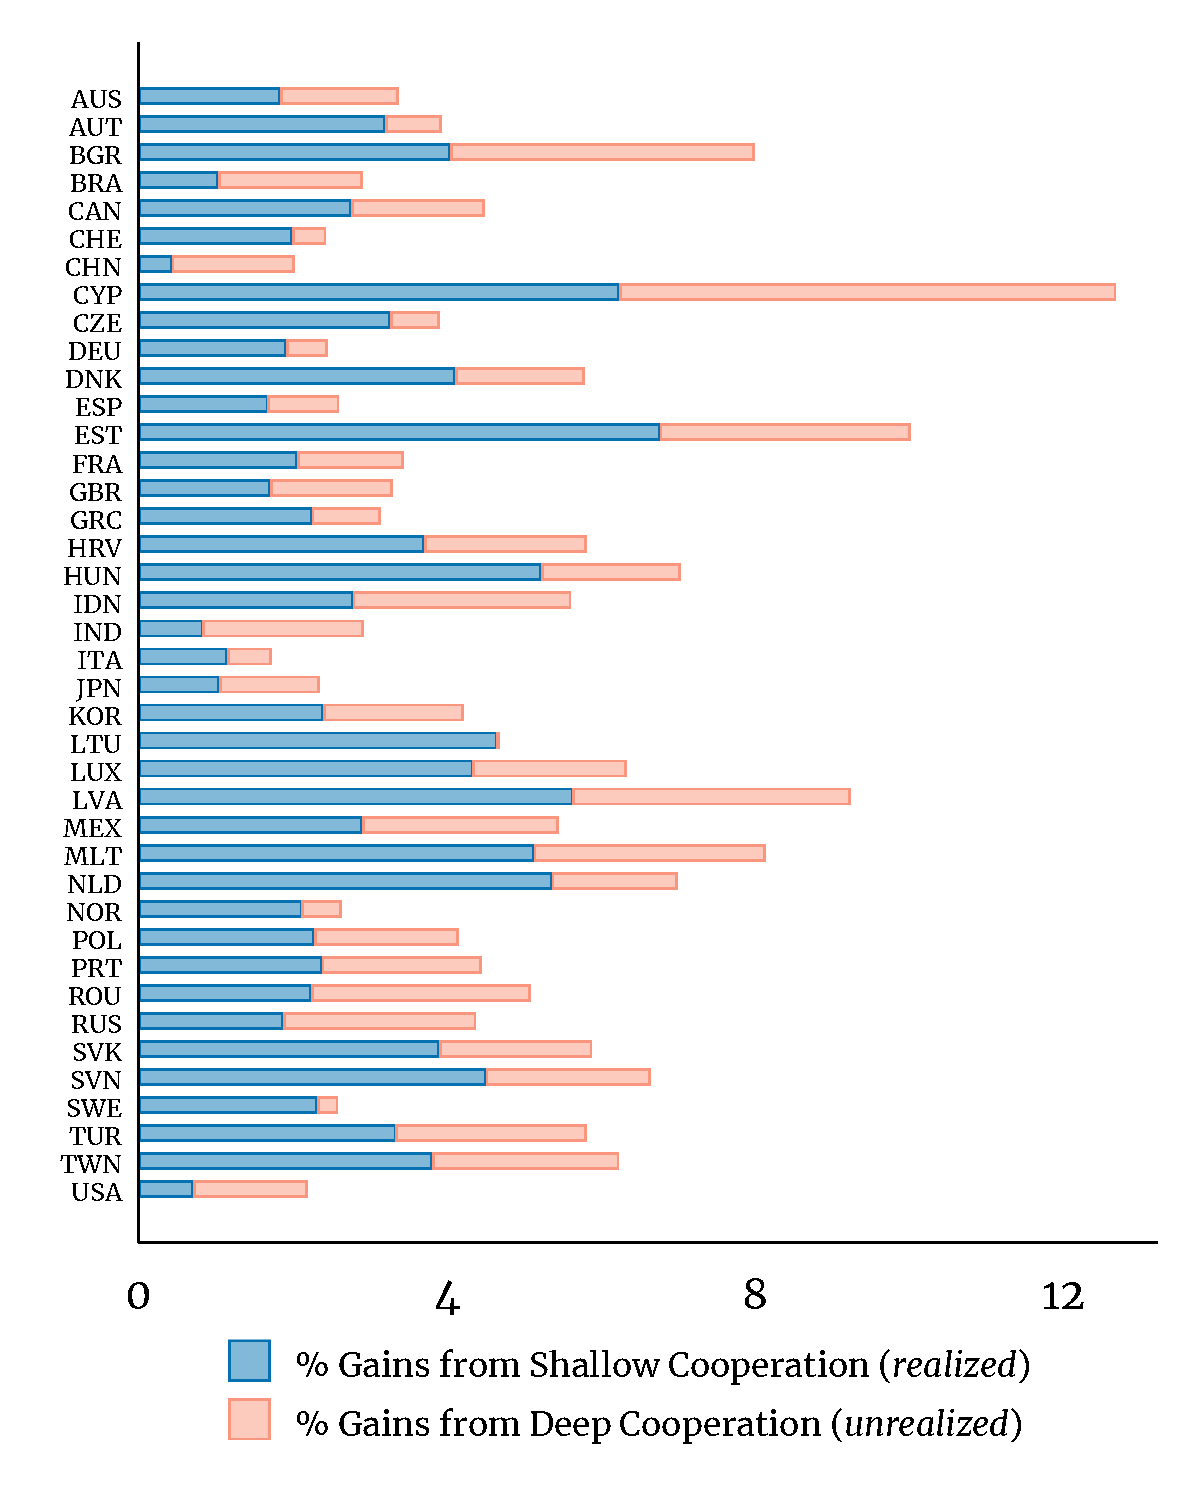
\includegraphics[scale=0.85]{stata_output/Figure_2}\vspace*{-20pt}
\par\end{centering}
\noindent\begin{minipage}[t]{1\columnwidth}%
\begin{spacing}{0.8}
\emph{\footnotesize{}Note}{\footnotesize{}: The data source is the
2014 World Input-Output Database (WIOD, \citet{timmer2015illustrated}).
Welfare effects are computed under restricted entry. The gains from
}\emph{\footnotesize{}deep cooperation}{\footnotesize{} correspond
to welfare gains when moving from the status quo to the globally efficient
equilibrium in which all countries coordinate their corrective Pigouvian
subsides. The gains from }\emph{\footnotesize{}shallow cooperation}{\footnotesize{}
correspond to the avoided welfare losses when moving from the status
quo to a non-cooperative equilibrium where all countries adopt Nash
trade taxes and subsidies. }
\end{spacing}
%
\end{minipage}
\end{figure}

The welfare gains from shallow cooperation are, on average, 3.2\%.
That is, the average country is poised to lose 3.2\% of its real income
if trade taxes are counterfactually raised to their non-cooperative
level everywhere. The existing nexus of shallow agreements have already
materialized these gains. The prospective gains from deep cooperation
are 1.6\% under restricted entry. That is, if countries can agree
to a reciprocal implementation of markup-correcting industrial policies,
they can boost their real income by an additional 1.6\%. Similar but
larger welfare gains will occur under free entry. 

Our estimated gains from shallow cooperation relate to the theoretical
arguments in \citet{bagwell2001domestic,bagwell2004economics}. As
explained earlier, shallow cooperation is sufficient for global efficiency
if $(i)$ $Cov\left(\mu_{k},\sigma_{k}\right)\geq0$, or $(ii)$ governments
play a one-shot game where they simultaneously choose and implement
their best-policy response with the belief that others do the same.
Our micro-level estimation rejected the former condition. Exhaustive
literature on the history of international policy coordination disputes
the latter condition. If we suspect that governments move sequentially
in the implementation stage and are not convinced about reciprocity
in policy implementation, then deep cooperation is necessary for global
efficiency.

\subsubsection{A Stronger Case for International Cooperation}

The standard argument for international cooperation recognizes that
governments can reap short-term gains if they adopt non-cooperative
trade taxes. But these short-term gains will turn into losses if trading
partners retaliate. The standard argument may, thus, fail to deter
a short-sighted government from taking the non-cooperative route.
After all, from the lens of traditional theories, the only way to
reap short-term welfare gains (relative to the status quo) is to adopt
non-cooperative trade restrictions and hope for delayed retaliation. 

Our quantitative analysis unveils a stronger augment for international
cooperation. Starting from the status quo, a government seeking welfare
improvements has two options: (1) engage in a coordinated industrial
policy effort, or (2) raise non-cooperative trade taxes to reap short-lived
ToT benefits. We find that the former option not only delivers sustainable
welfare gains but strictly dominates the latter option even before
we adjust for the cost of retaliation.

This point is illustrated in Figure (\ref{fig: multilateral vs unilateral}).
The \emph{x-axis }corresponds to the unrealized gains from deep cooperation.
The \emph{y-axis} corresponds to the maximal short-term gains from
(non-cooperative) unilateral policies, which transpire before retaliation.
For most economies, the unrealized gains from deep cooperation dominate
even the short-term gains from unilateral policy interventions. This
finding indicates that the spillover gains from corrective policies
in the rest of the world exceed the short-term ToT gains from non-cooperative
taxes---echoing our earlier claim that the ToT gains from policy
are limited in scope, even before retaliation.\footnote{Interestingly, the gains from deep cooperation favor small countries
that have a comparative disadvantage in high-returns-to-scale (or
high-profit) industries, \emph{e.g.}, Estonia, Malta, and Slovenia.
The intuition is that these countries depend relatively more on imported
varieties in high-returns-to-scale industries and under deep cooperation,
these industries are subsidized across the globe.}

\begin{figure}[!tbh]
\caption{\label{fig: multilateral vs unilateral} {\large{}Deep cooperation
vs. unilateral policy interventions}}

\begin{centering}
\hspace*{-25pt}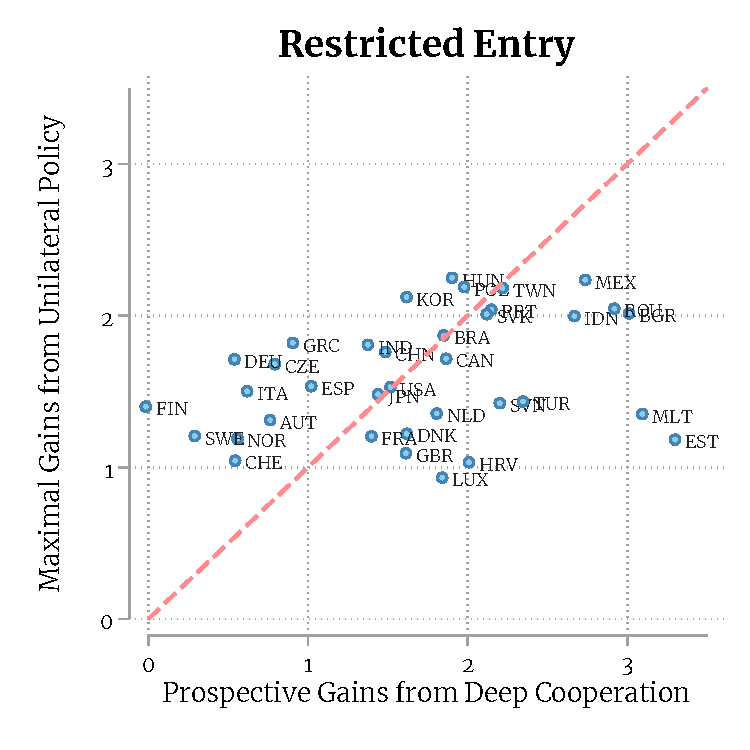
\includegraphics[scale=0.65]{stata_output/Figure_3A}\enskip{}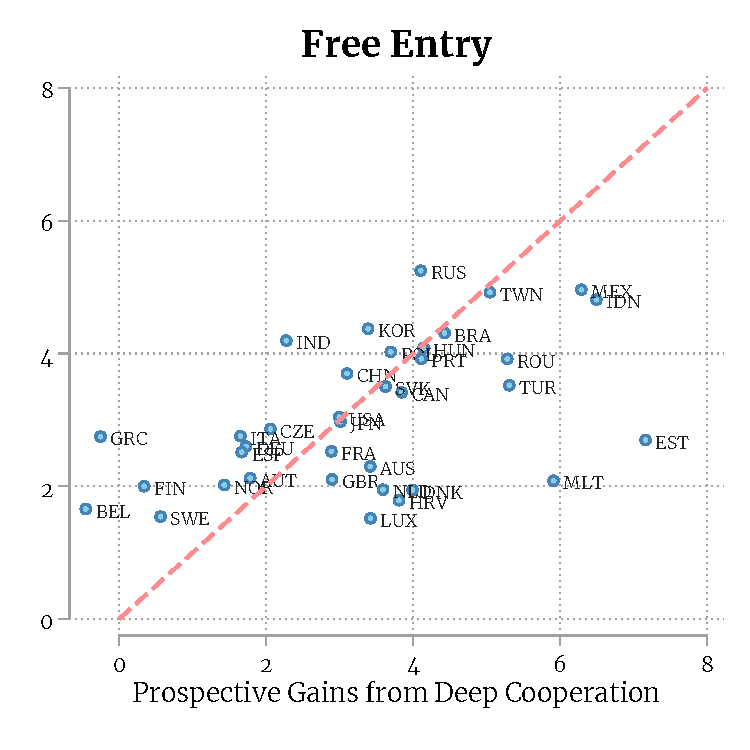
\includegraphics[scale=0.65]{stata_output/Figure_3B}\vspace{-0.1in}
\par\end{centering}
\noindent\begin{minipage}[t]{1\columnwidth}%
\begin{spacing}{0.8}
{\footnotesize{}Note: The data source is the 2014 World Input-Output
Database (WIOD, \citet{timmer2015illustrated}). The gains from 1st
best non-cooperative policy are the gains when each country implements
the policy characterized by Theorem 1, and the rest of the world is
passive. The gains from global cooperation correspond to a scenario
where all countries forgo trade taxation and apply industrial subsidies
that restore marginal cost pricing.}
\end{spacing}
%
\end{minipage}
\end{figure}


\subsection{Sensitivity Analysis}

In online Appendix \ref{sec: Gains Robustness}, we recalculate the
gains from policy under several alternative specifications. First,
we recompute the gains assuming that the data-generating process is
a \emph{\citeauthor{Melitz2003}-Pareto} model. Second, we recompute
the gains based on alternative values for $\sigma_{k}$ and $\mu_{k}$,
which are estimated via a two-ways fixed effects estimation (as reported
in online Appendix \ref{sec: Two-Ways FE Estimation}). Lastly, we
recompute the gains from policy under a more conservative set of values
assigned to $\mu_{k}$ and $\sigma_{k}$ in services. In all cases,
trade policy turns out to be a poor second-best instrument for resorting
allocative efficiency. Another noteworthy observation is that accounting
for firm-selection effects \`a la \citet{Melitz2003}, magnifies
the gains from (first-best) optimal policies. However, these greater
gains are primarily driven by the larger misallocation-correcting
gains. If anything, second-best trade taxes/subsidies are even less
effective at replicating the first-best policy gains in the presence
of firm-selection into export markets.\bigskip{}

\emph{What parameter values would imply larger gains from policy?$\quad$}We
analyze this question in online Appendix \ref{sec: Artificial Param},
noting that the gains from optimal policy are increasing in two statistics:
$(i)$ the cross-industry variance of the scale elasticities, $\text{Var}\left(\log\mu_{k}\right)$,
and $(ii)$ the average of the (inverse) trade elasticities, $\mathbb{E}\left[\frac{1}{\sigma_{k}-1}\right]$.
In online Appendix \ref{sec: Artificial Param}, we adjust our estimated
parameter values to artificially increase both of these statistics
and recompute the gains from policy under these artificial parameter
values. The results are reported in Figure \ref{fig: Artificial Parameters}
of the same appendix. They reveal that the gains from optimal policy
nearly double for all countries if we artificially increase $\text{Var}\left(\log\mu_{k}\right)$
by a factor of about three. The policy gains for different countries,
however, exhibit different degrees of sensitivity to an artificial
increase in $\mathbb{E}\left[\frac{1}{\sigma_{k}-1}\right]$---with
the gains for larger countries like the U.S. or China being noticeably
less sensitive. The intuition is that $\text{Var}\left(\log\mu_{k}\right)$
governs the gains from correcting misallocation, whereas $\mathbb{E}\left[\frac{1}{\sigma_{k}-1}\right]$
regulates the extent to which countries can improve their ToT. For
large countries, where trade accounts for a smaller fraction of the
GDP, there is less scope for raising real GDP via ToT improvements---hence,
the lower sensitivity of policy gains to $\mathbb{E}\left[\frac{1}{\sigma_{k}-1}\right]$.

\section{Concluding Remarks }

Correcting  misallocation driven by economies of scale has often served
as a justification for controversial trade and industrial policy practices.
Yet we know surprisingly little about the efficacy of trade and industrial
policy in increasing returns to scale industries. Against this backdrop,
we employed micro-level trade data to examine the consequences of
industry-level scale economies, offering insights into the effectiveness
of various policy interventions. Our findings reveal that trade restrictions
are a poor second-best policy choice for correcting misallocation
in the domestic economy. Unilateral industrial policy measures can
be equally ineffective, as they lead to immiserizing growth. Meanwhile,
industrial policies coordinated internationally via deep agreements
deliver welfare gains that are more transformative than any unilateral
policy alternative.

The scale elasticity estimates obtained in this paper can be used
for further exploration in several areas. First, our scale elasticity
estimates can help disentangle the relative contribution of scale
economies and Ricardian comparative advantage to inter-sectoral specialization.
This is an old topic of interest, for which our empirical understanding
is somewhat limited. Second, our estimates can perhaps shed fresh
light on the puzzlingly large income gap between advanced and emerging
economies. Economists have long hypothesized that a fraction of this
income gap stems from specialization across low- and high returns-to-scale
industries. Empirical assessments of this hypothesis have proven difficult
due to a lack of comprehensive estimates for industry-level scale
elasticities. Our micro-level estimates, however, can pave the way
for such explorations. Finally, we document a negative cross-industry
correlation between trade and scale elasticities. This relationship
is crucial for policy evaluation in open economies as it points to
a tension between the terms-of-trade and allocative efficiency objectives.
While our theoretical model is purposely agnostic about the origins
of this negative relationship, further exploration into this matter
is warranted.

\begin{singlespace}
{\small{}\bibliographystyle{aea}
\bibliography{LL2023}
}{\small\par}
\end{singlespace}

\end{document}
